
\begin{frame}
\frametitle{Applications are important}
\begin{itemize}
\item Provide motivation for basic research
\begin{itemize}
\item Which constraints, methods are needed
\end{itemize}
\item Provide realistic benchmark problems
\begin{itemize}
\item Easy to optimize for pointless results
\end{itemize}
\item Shows that research has potential benefits
\begin{itemize}
\item Much easier to convince funding agencies
\end{itemize}
\item Typically much easier to explain than solver internals
\begin{itemize}
\item Interest students, do outreach
\end{itemize}
\end{itemize}
\end{frame}

\begin{frame}
\frametitle{Main Application Areas for CP}
\begin{itemize}
\item Scheduling
\begin{itemize}
\item By far the largest application area
\end{itemize}
\item Product Configuration
\begin{itemize}
\item No longer much of a research focus
\item Start with Ulrich Junker's chapter in \href{https://www.sciencedirect.com/bookseries/foundations-of-artificial-intelligence/vol/2/suppl/C}{Handbook of Constraint Programming}
\end{itemize}
\item Rostering and Assignment
\begin{itemize}
\item Propagation is very powerful
\item Start with Demirovi\`{c}, E., Stuckey, P.J. (2018). \href{https://link.springer.com/chapter/10.1007/978-3-319-93031-2_10}{Constraint Programming for High School Timetabling: A Scheduling-Based Model with Hot Starts}. CPAIOR 2018.
\end{itemize}
\item Software/Hardware Design and Testing
\begin{itemize}
\item Sometimes using specialized domains (uint32)
\item Start with Arnaud Gotlieb video \url{https://www.youtube.com/watch?v=E1Seayx3eXU}
\end{itemize}
\item Transportation
\begin{itemize}
\item Hybrids with other techniques
\item Start with Augustin Delecluse, Pierre Schaus, and Pascal Van Hentenryck. \href{https://drops.dagstuhl.de/entities/document/10.4230/LIPIcs.CP.2022.19}{Sequence Variables for Routing Problems}. CP 2022.
\end{itemize}
\end{itemize}
\end{frame}

\mode<all>{
\section{CP and Scheduling Literature Survey}

\begin{frame}
\frametitle{A Survey of the Existing Literature}
\begin{itemize}
\item Joint work with Cemalettin Öztürk, MTU
\item What is out there
\item Where to start
\item Where to publish
\item I'm interested in some specific topic, what is relevant
\end{itemize}
\end{frame}

\begin{frame}
\frametitle{Methodology}
\begin{itemize}
\item Manually curated list of works, somewhat inclusive
\item Starting with bibtex files
\item Citation links through \href{https://opencitations.net/}{OpenCitations} (open access)
\item Content analysis on local copies of pdf files
\item Closure of domain by analyzing missing cited and citing works 
\item Limited manual analysis of works (datasets, code)
\item Results presented as LaTeX documents
\item Open source analysis on git: \url{https://hsimonis.github.io/pthg24/}
\end{itemize}
\end{frame}

\begin{frame}
\frametitle{Overall Analysis (Based on 671 Works)}
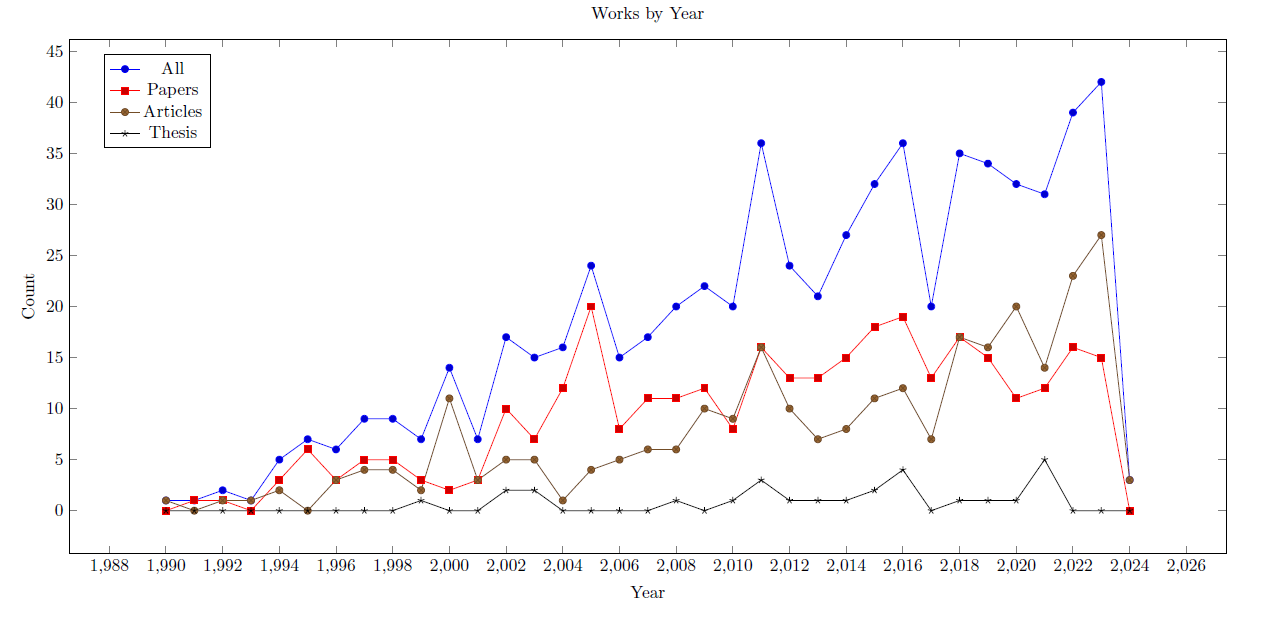
\includegraphics[width=\textwidth]{survey/worksbyyear}
\end{frame}

\begin{frame}
\frametitle{Origin of Papers/Articles}
\begin{tabular}[t]{cc}
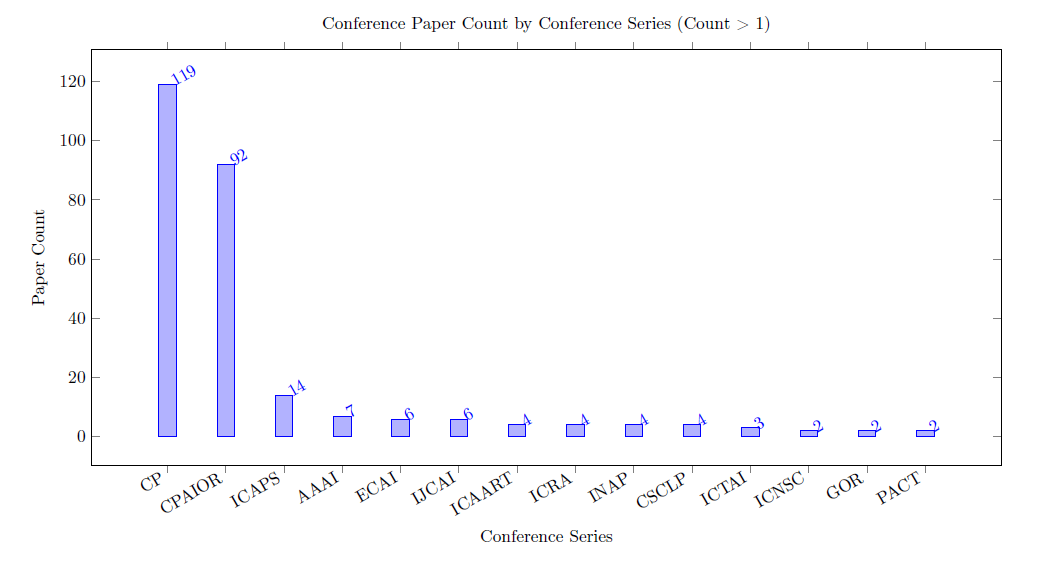
\includegraphics[width=.45\textwidth]{survey/conferences}
& 
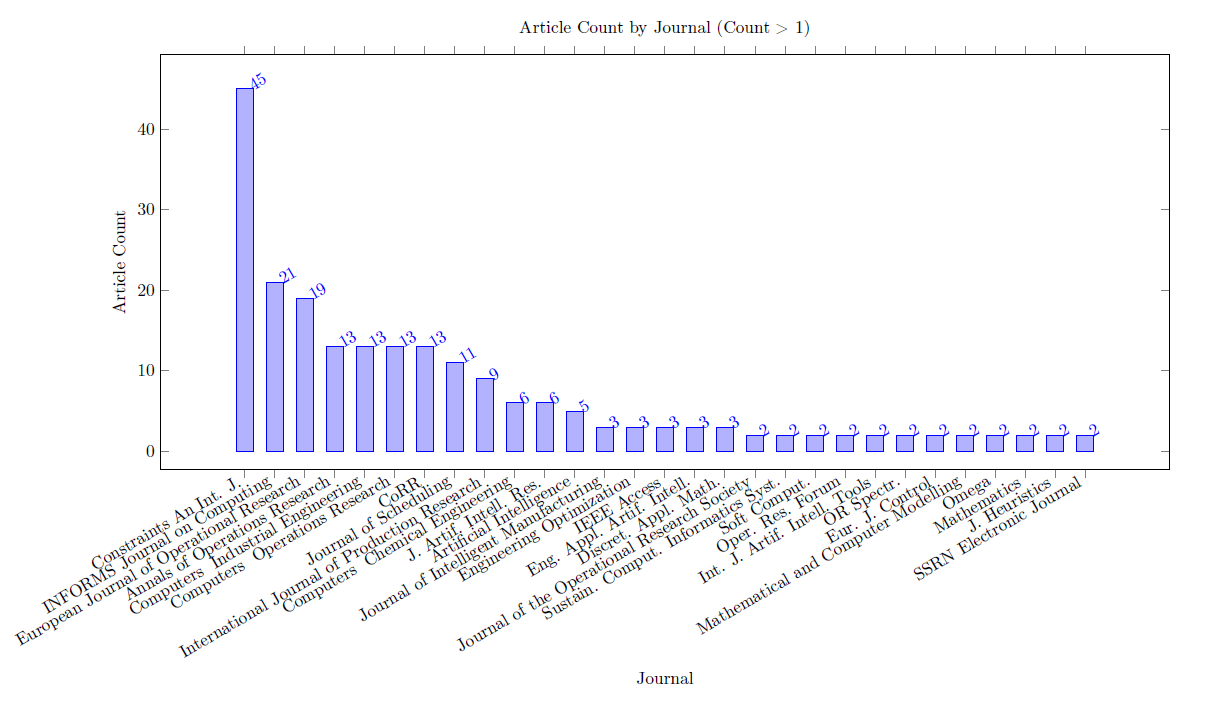
\includegraphics[width=.55\textwidth]{survey/journals}
\end{tabular}
\end{frame}

\begin{frame}
\frametitle{Most Recent Articles}
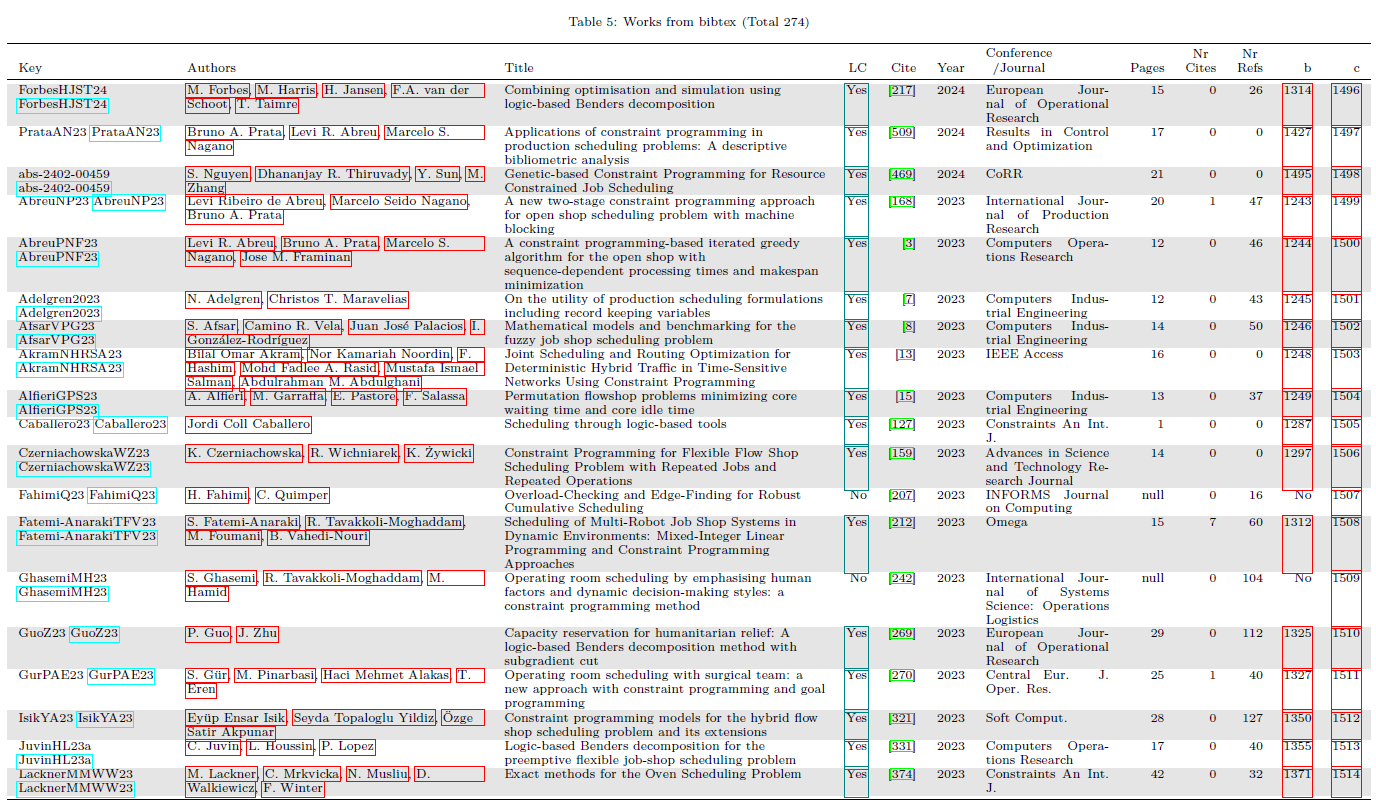
\includegraphics[width=\textwidth]{survey/mostrecentarticles}
\end{frame}

\begin{frame}
\frametitle{Automatically Extracted Article Features}
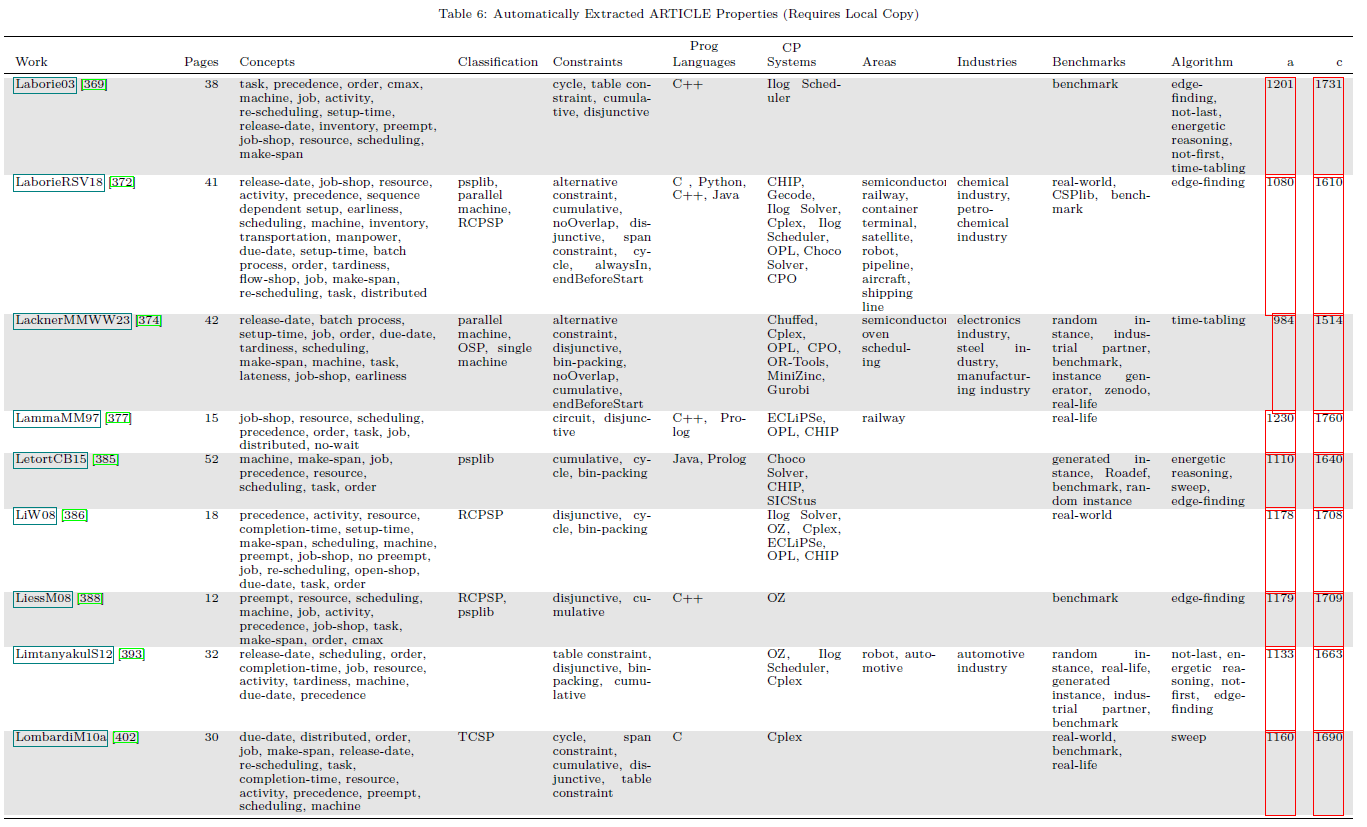
\includegraphics[width=\textwidth]{survey/extracted}
\end{frame}

\begin{frame}
\frametitle{Manually Extracted Article Features}
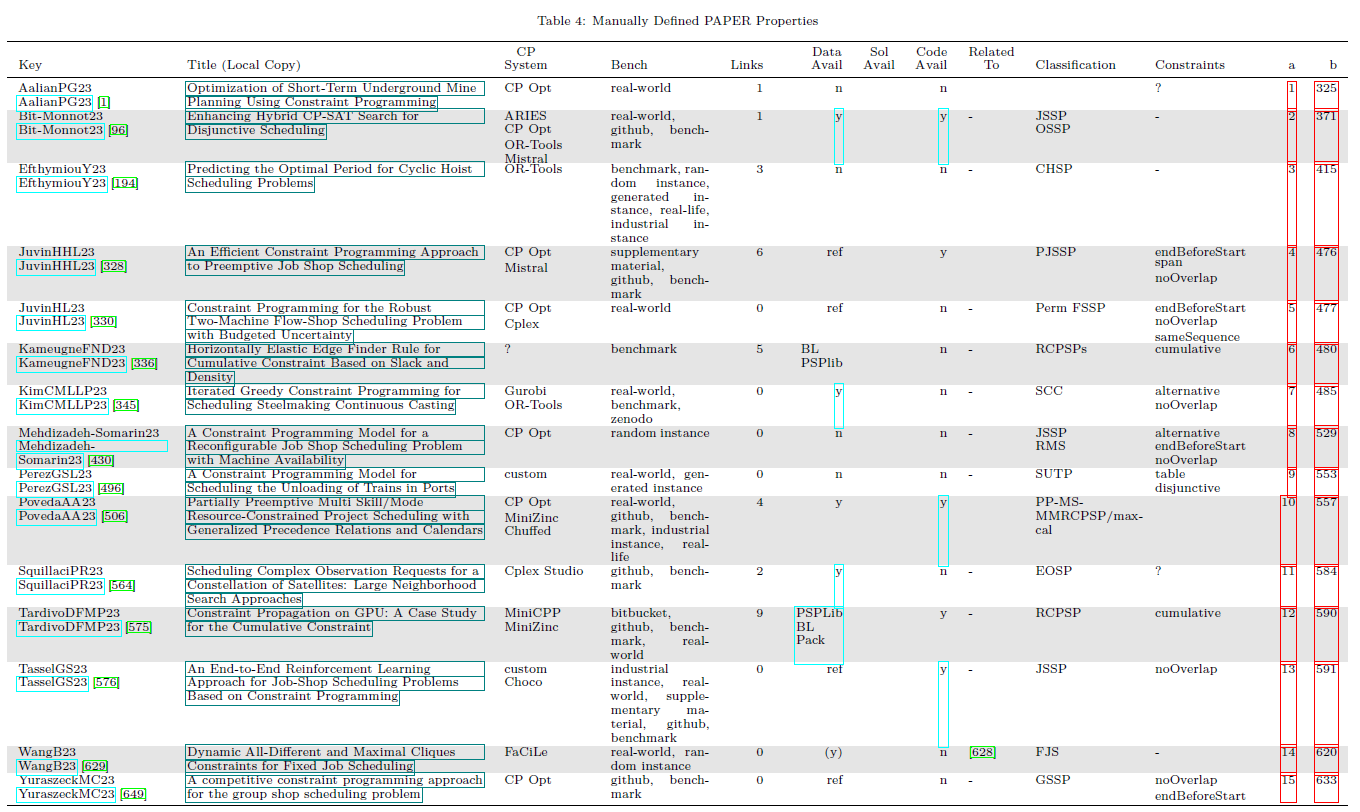
\includegraphics[width=\textwidth]{survey/manual}
\end{frame}


\begin{frame}
\frametitle{Extracted Features: Application Areas}
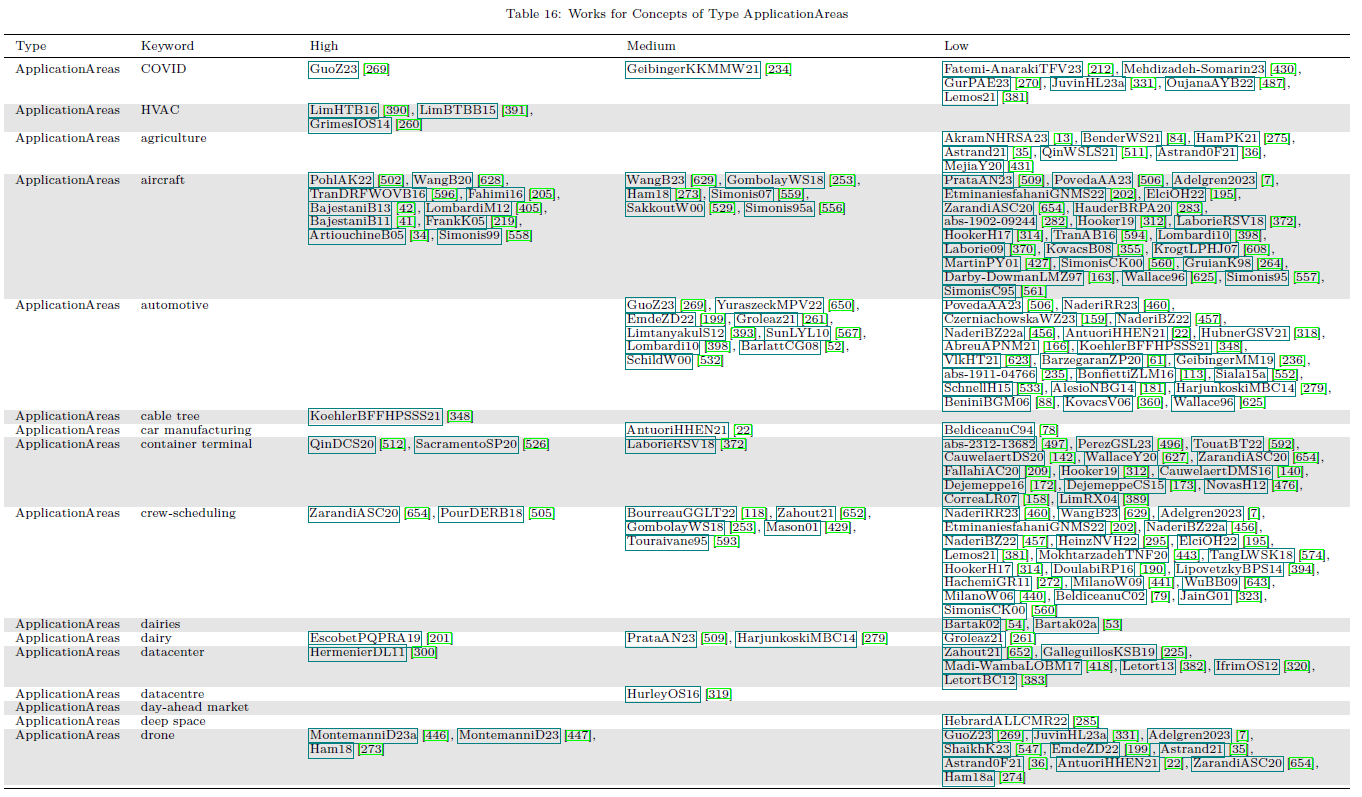
\includegraphics[width=\textwidth]{survey/applicationareas}
\end{frame}

\begin{frame}
\frametitle{Prolific Authors}
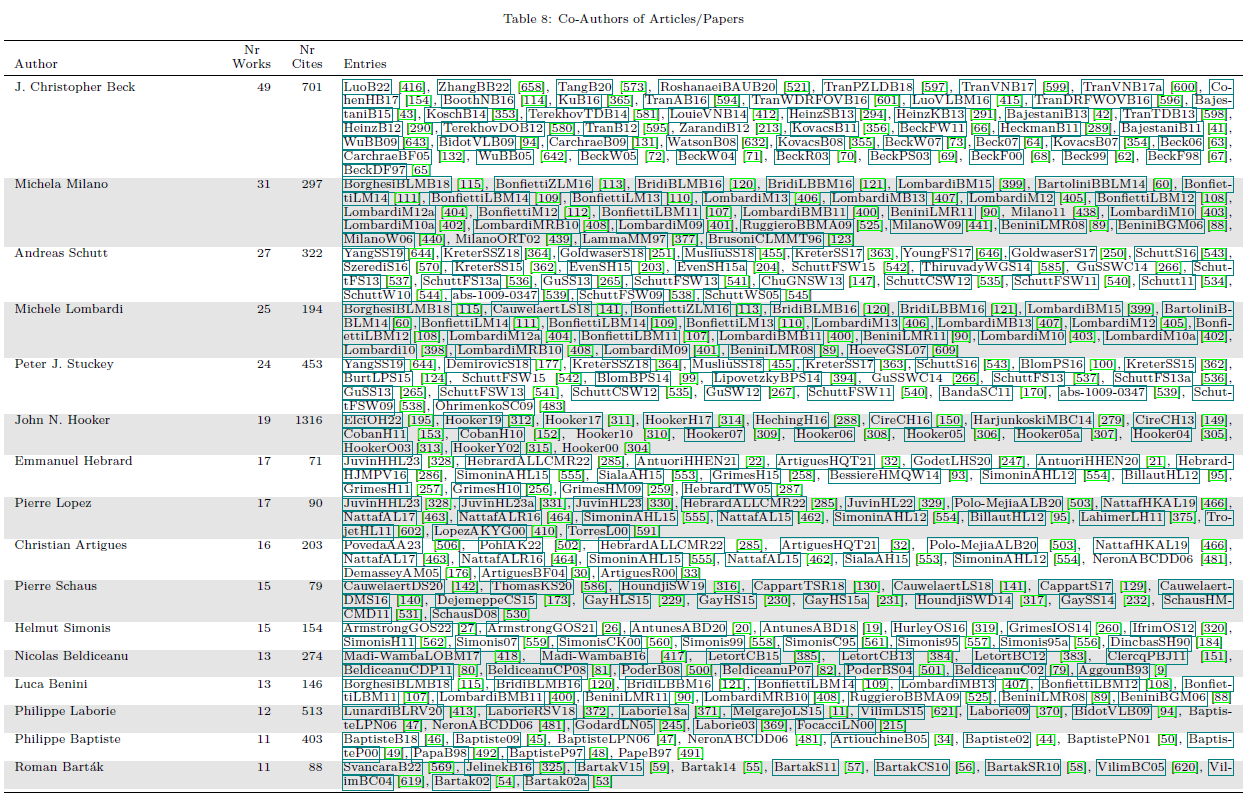
\includegraphics[width=\textwidth]{survey/authors}
\end{frame}


\begin{frame}
\frametitle{Limitations}
\begin{itemize}
\item Limited coverage by \href{https://opencitations.net/}{OpenCitations}
\item Difficult to have local access to some publication types (book, incollection)
\item Heavily biased towards publications in English
\item More powerful NLP analysis of works possible?
\end{itemize}
\end{frame}

\begin{frame}
\frametitle{Problem: Count for Most Cited Papers}
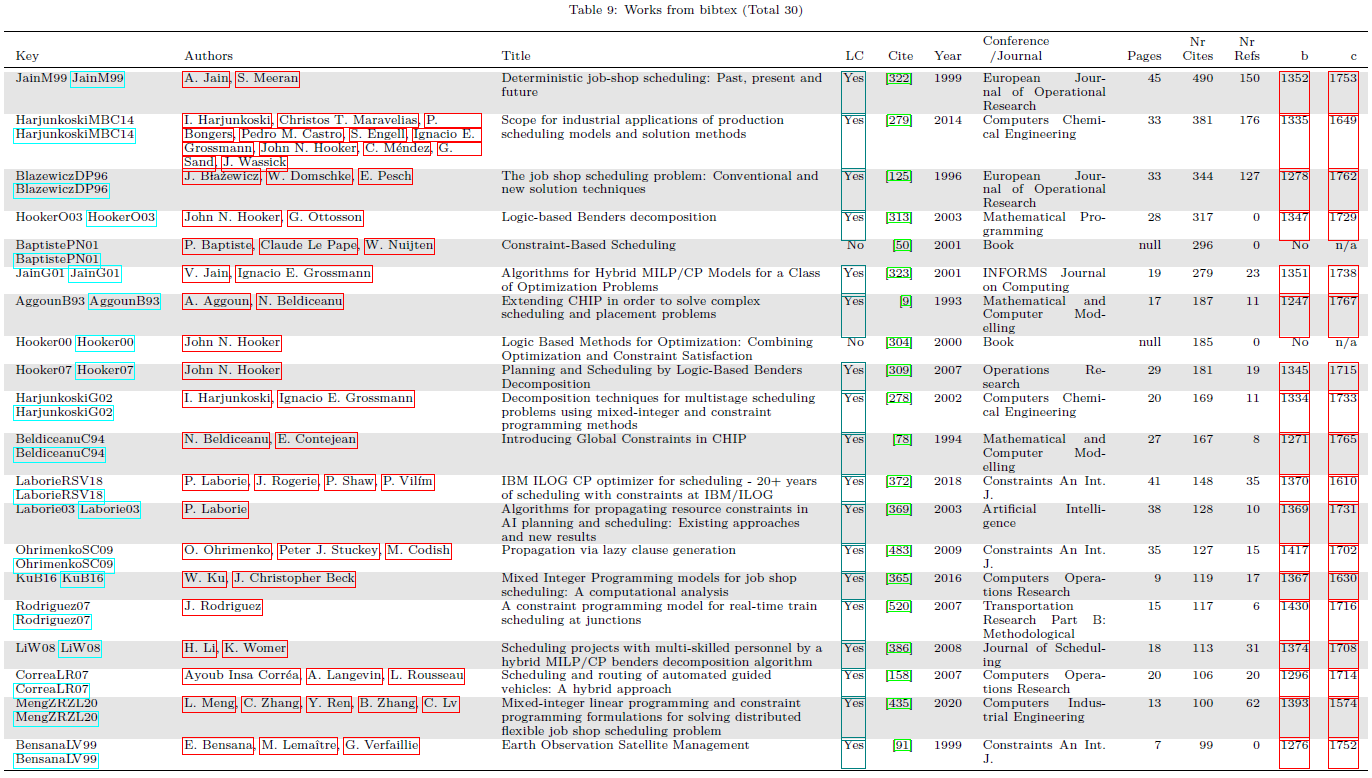
\includegraphics[width=\textwidth]{survey/mostcited}
\end{frame} 

\begin{frame}
\frametitle{OpenCitation Count Compared to Google Scholar}
\begin{tabular}{llrrr}\toprule
Key & Type & Google & OC & Ratio \\ \midrule
JainM99          & article & 1116 & 490 & 2.28\\
HarjunkoskiMBC14 & article &  588 & 381 & 1.54\\
BlazewiczDP96    & article &  796 & 344 & 2.31\\
BaptistePN01     & book    & 1039 & 296 & 3.51\\
AggounB93        & article &  502 & 187 & 2.68\\
LaborieRSV18     & article &  309 & 148 & 2.09\\
BensanaLV99      & article &  251 &  99 & 2.54\\
DincbasSH90      & article &  271 &  86 & 3.15\\
Thorsteinsson01  & paper   &  205 &  67 & 3.06\\
\midrule
DincbasSH88      & paper   &  287 &   0 & \frownie{}\\
\bottomrule
\end{tabular}
\end{frame}
 


\begin{frame}
\frametitle{Problem: Citation Count Distribution}
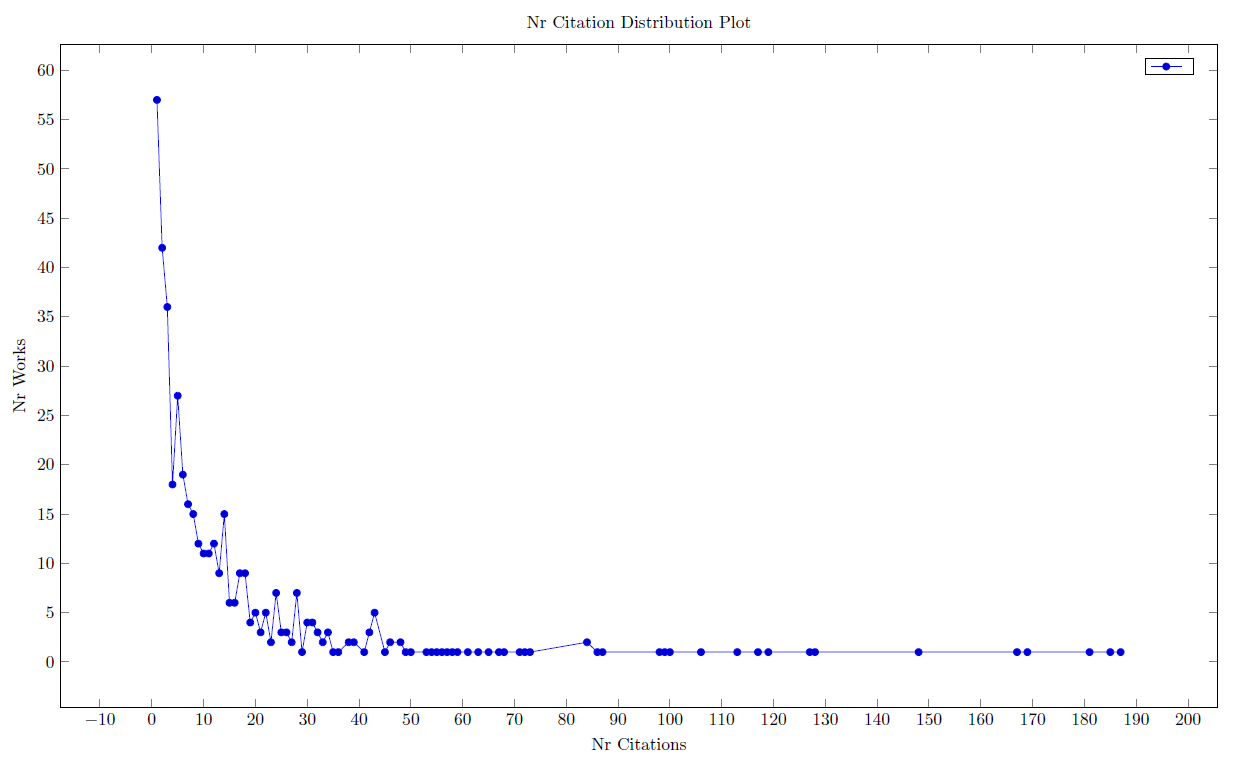
\includegraphics[width=.8\textwidth]{survey/citationcount}
\end{frame}

\begin{frame}
\frametitle{Reuse Example: Survey of Car Sequencing}
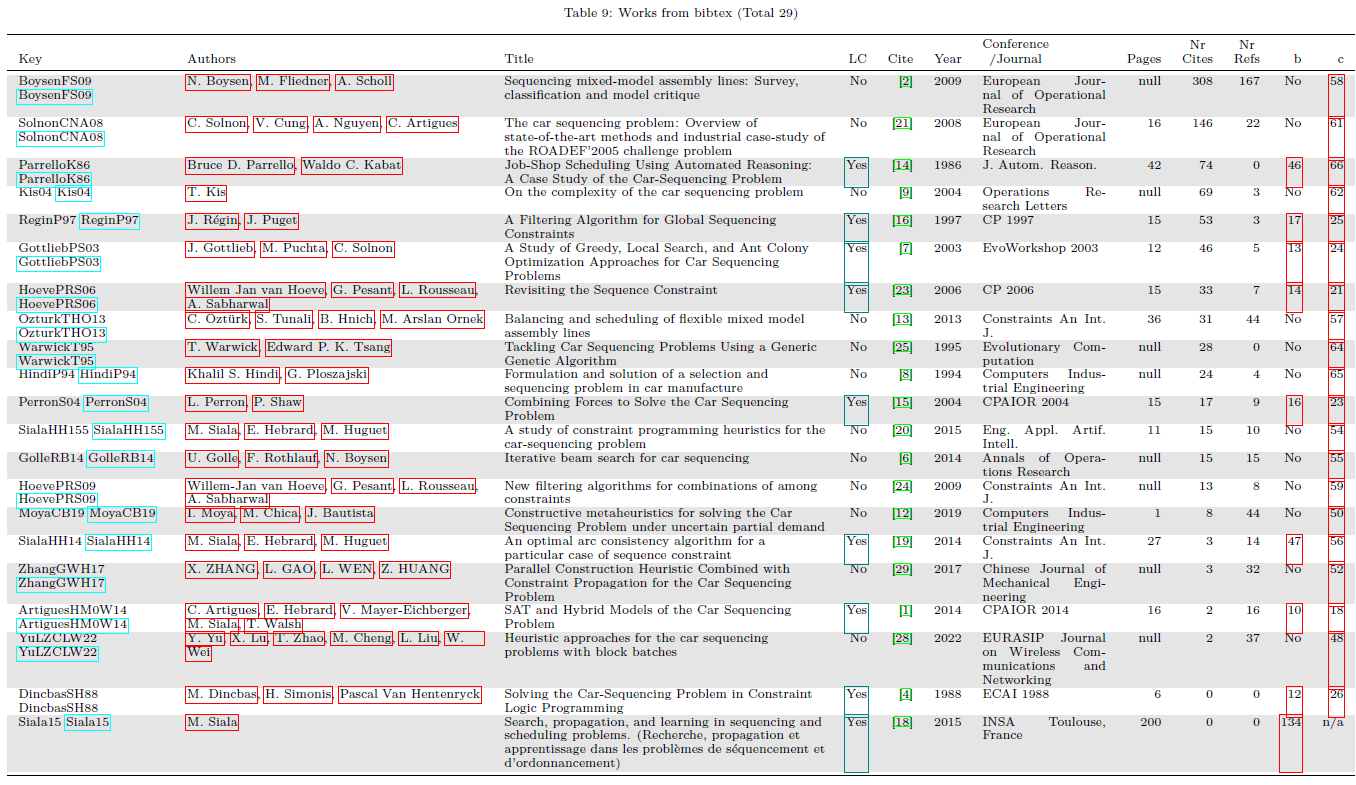
\includegraphics[width=\textwidth]{survey/carsequencing}
\end{frame}



}

% \begin{frame}
% \frametitle{Take-Away Message}
% \begin{itemize}
% \item Problem led research can be fun and rewarding
% \item Very different types of applications and domains
% \item From research prototypes to fielded systems
% \item Variety of tools and methods
% \item Provides structure to fundamental research
% \end{itemize}
% \end{frame}

\begin{frame}
\frametitle{More Detailed Example Applications}
\begin{itemize}
%\item Flexible Flow-Shop with Transportation Times 
%\begin{itemize}
%\item J\&J, studies future factory design
%\end{itemize}
\item Production Planning and Scheduling
\begin{itemize}
\item Siemens Energy, part of ASSISTANT project
\end{itemize}
\item Outpatient Waitlist Management 
\begin{itemize}
\item Working within health service
\end{itemize}
\item Elevator Maintenance Planning and Scheduling
\begin{itemize}
\item Combination with simulation
\end{itemize}
%\item CAT Constraint Acquisition
%\begin{itemize}
%\item Part of ASSISTANT EU project, aimed at scheduling
%\end{itemize}
\item Selection of other problem types
\begin{itemize}
\item Only summary slide shown
\end{itemize}
\end{itemize}
\end{frame}

%\mode<all>{\section{Hybrid Flexible Flowshop with Transportation Times}


\begin{frame}
\frametitle{Joint work with}
\begin{itemize}
\item Michele Garraffa
\item Barry O'Sullivan
\item Eddie Armstrong (J\&J Research, Limerick)
\end{itemize}
\end{frame}

\subsection{Introduction}

\begin{frame}
\frametitle{Real-World Problem}
\begin{itemize}
\item Manufacturing Industry
\item Move away from dedicated, high volume standard production
\item Allow for increasing customization of product to customer needs
\item Take advantage of more flexible, universal machines
\item Decentralize production
\end{itemize}
\end{frame}

\begin{frame}
\frametitle{Research Challenges}
\begin{itemize}
\item Consider transport time in flowshop scheduling
\item Choose appropriate technology to solve problem
\item Study realistic scenarios at scale
\end{itemize}
\end{frame}

% \begin{frame}
% \frametitle{What we will discuss}
% \begin{itemize}
% \item New variant of known scheduling problem
% \begin{itemize}
% \item Hybrid Flexible Flowshop with Transportation Times
% \item Solved with different approaches
% \begin{itemize}
% \item CP (4 Versions)
% \item MIP (5 Versions)
% \item Local Search
% \end{itemize}
% \item Spoiler: CP works well, MIP not so much
% \end{itemize}
% \item Factory layout problem
% \begin{itemize}
% \item How does the layout affect the scheduling?
% \item Compare different high level design scenarios
% \end{itemize}
% \end{itemize}
% \end{frame}

\begin{frame}
\frametitle{A bit of Background}
\begin{textblock*}{4cm}(11cm,2cm)

\includegraphics[width=4cm]{imagesjj/1000px-Johnson_and_Johnson_Logo.png}
\end{textblock*}
\begin{textblock*}{4cm}(11cm,4cm)

\includegraphics[width=4cm]{imagesjj/confirm.png}
\end{textblock*}
\begin{itemize}
\item Johnson\&Johnson is a large multi-national company
\begin{itemize}
\item Strong production and research presence in Ireland
\item Focus on consumer health, medical devices, pharmaceuticals
\end{itemize}
\item Confirm
\begin{itemize}
\item Irish National SFI Centre focussed on Manufacturing
\item Includes groups from multiple universities
\item Our focus is on analytics/optimization
\item Complements our work in the Insight SFI Centre for Data Analytics
\end{itemize}
\end{itemize}
\end{frame}

\subsection{Problem Description}

\begin{frame}
\frametitle{Flexible Factory Structure (Including Transport Between Machines)}
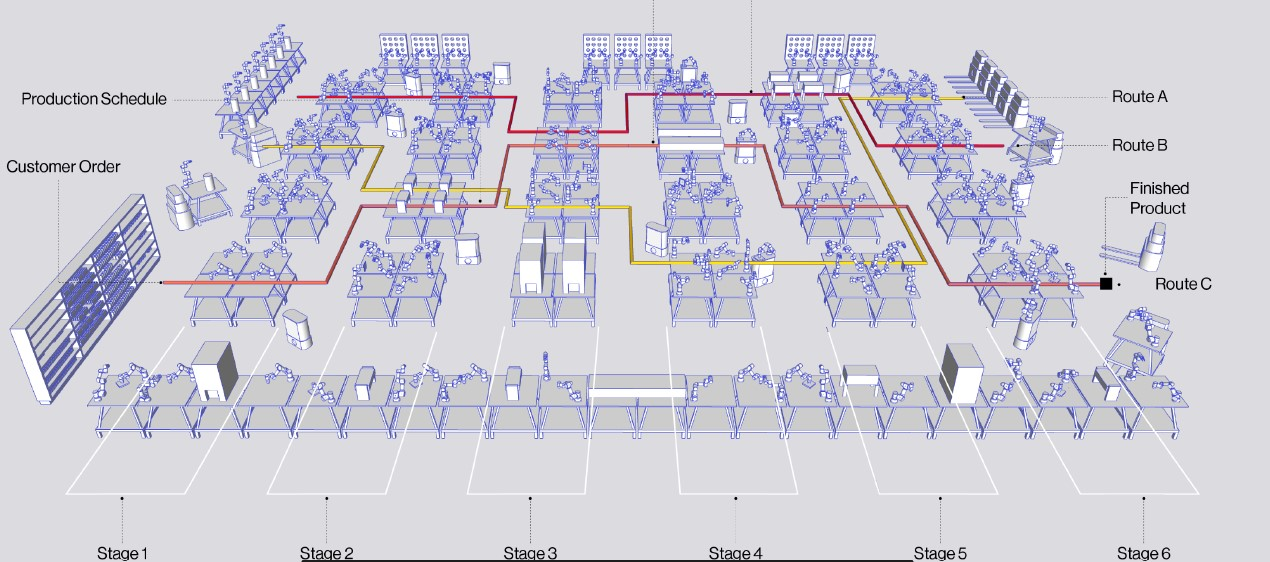
\includegraphics[width=14cm]{imagesjj/factory}
\end{frame}

\begin{frame}
\frametitle{Main Elements of Problem}
\begin{itemize}
\item Flow shop
\begin{itemize}
\item Jobs run through production in the same sequence
\end{itemize}

\item Hybrid
\begin{itemize}
\item Multiple, identical machines available in each stage
\end{itemize}

\item Flexible
\begin{itemize}
\item Some production stages may be skipped for certain jobs
\end{itemize}

\item Transportation Time
\begin{itemize}
\item Time for transport between stage is significant, but not a resource limit
\item Many robots to handle transport tasks
\item Typical machine layout in lanes
\end{itemize}

\item Objective makespan
\begin{itemize}
\item Production not driven by due dates
\end{itemize}
\end{itemize}
\end{frame}

% \begin{frame}
% \frametitle{Why is this interesting?}
% \begin{itemize}
% \item Industrial Use Case

% \item Increased complexity over existing hybrid flexible flowshop

% \item Machines in each stage are no longer exchangeable in schedule
% \begin{itemize}
% \item Reduced symmetry
% \item But also preferred paths through factory
% \end{itemize}

% \end{itemize}
% \end{frame}

% \begin{frame}
% \frametitle{Not Considered in this Study}
% \begin{itemize}
% \item Sequence dependent setup times
% \begin{itemize}
% \item Machines are highly flexible, do not require setup times
% \end{itemize}

% \item Buffer space
% \begin{itemize}
% \item Manufactured items are quite small
% \item Trays can be stacked in front of machines
% \end{itemize}

% \item Different production speed on machines of same stage
% \begin{itemize}
% \item Assumes same generation of machines within each stage
% \item (Different stages have different processing
% \end{itemize}

% \item Resource limits on transport
% \begin{itemize}
% \item No congestion in transport lanes
% \item Enough robots to keep material flowing through plant
% \end{itemize}
% \end{itemize}
% \end{frame}

\begin{frame}
\frametitle{Objectives of Project}
\begin{itemize}
\item Identify best tools to schedule new plant
\begin{itemize}
\item Explore variety of different approaches and techniques
\item Do not just focus on your preferred solution method/solver
\end{itemize}

\item Answer some design questions before committing to one approach
\begin{itemize}
\item Is it better to have one or multiple facilities?
\item How far should the transport reach between lanes?
\item How can we exploit flexibility in new machines to offer better products?
\begin{itemize}
\item Semi custom production
\end{itemize}
\end{itemize}

\item Provide some quantitative comparison based on typical production data
\begin{itemize}
\item Not currently for operational scheduling
\end{itemize}

\end{itemize}
\end{frame}

\subsection{Models}

\begin{frame}
\frametitle{CP Models}
\begin{itemize}
\item Two main modelling alternatives
\begin{itemize}
\item Diffn model to handle machine choice
\item Interval Task Variables with optional tasks on all alternative machines
\end{itemize}

\item Transportation time handled by table constraint
\begin{itemize}
\item Transportation between machines for tasks of the same job
\item Much simpler case than sequence dependent setup
\end{itemize}

\item Precedences between tasks of jobs

\item Objective Cmax makespan

\end{itemize}
\end{frame}

\begin{frame}
\frametitle{CP Model Main Alternative}
\begin{tabular}{cc}
\scalebox{0.5}{
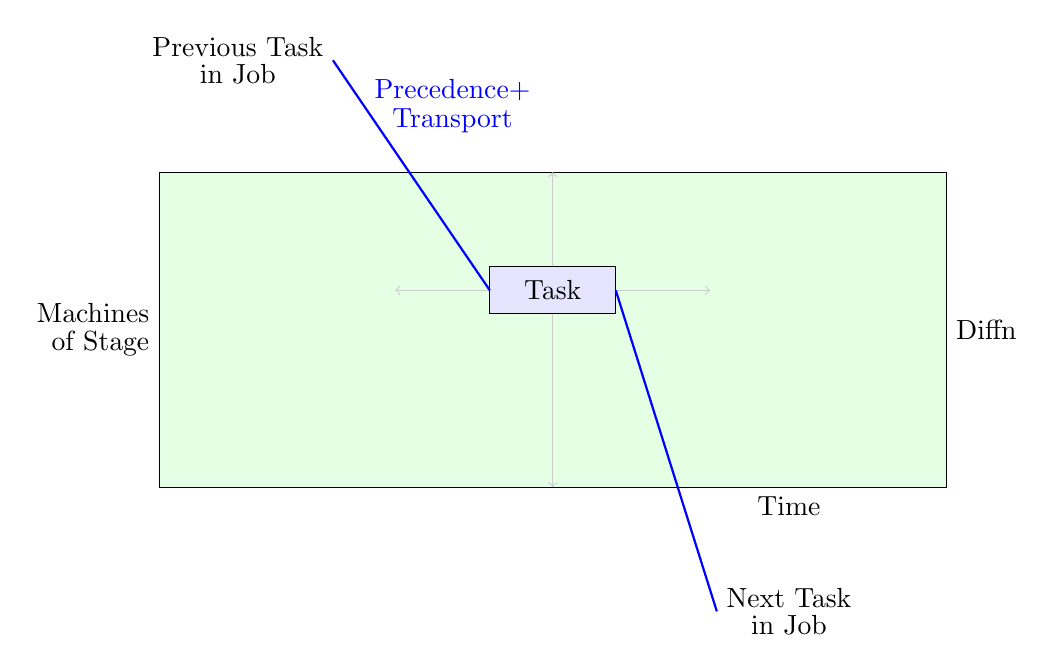
\begin{tikzpicture}
  \draw[draw=black,fill=green!10] (0,0) rectangle (10,4);
  \node[right] () at (10,2.0) {Diffn};
  \draw[black!20,<->] (3,2.5) -- (7,2.5);
  \draw[black!20,<->] (5,0) -- (5,4);
  \draw[fill=blue!10] (4.2,2.2) rectangle node {Task} (5.8,2.8);
  \node[below] (time) at (8,0) {Time};
  \node[left] (machine) at (0,2) {\shortstack[r]{Machines\\of Stage}};
  \node[above] (prev) at (1,5) {\shortstack{Previous Task\\in Job}};
  \node[above] (next) at (8,-2) {\shortstack{Next Task\\in Job}};
  \draw[thick,blue] (prev.east) -- node[pos=0.2,right] {\shortstack{Precedence+\\Transport}} (4.2,2.5);
  \draw[thick,blue] (next.west) -- (5.8,2.5);
\end{tikzpicture}
}
&
\scalebox{0.5}{
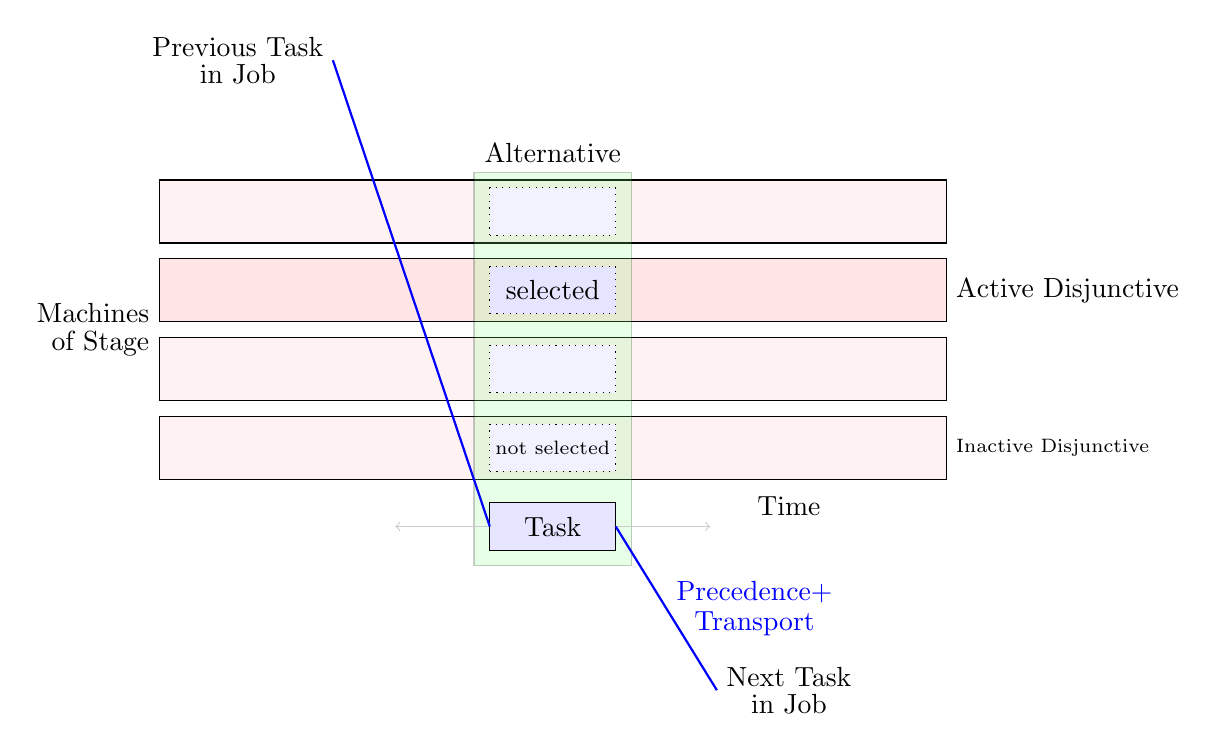
\begin{tikzpicture}
  \draw[draw=black,fill=red!5] (0,0.1) rectangle (10,0.9);
  \draw[draw=black,fill=red!5] (0,1.1) rectangle (10,1.9);
  \draw[draw=black,fill=red!10] (0,2.1) rectangle (10,2.9);
  \draw[draw=black,fill=red!5] (0,3.1) rectangle (10,3.9);
  \node[right] () at (10,2.5) {Active Disjunctive};
  \node[right] () at (10,0.5) {\scriptsize Inactive Disjunctive};
  \draw[fill=green!50,opacity=0.2] (4,-1) rectangle (6,4);
  \node[above] () at (5,4) {Alternative};
  \draw[dotted,fill=blue!5] (4.2,0.2) rectangle node {\scriptsize not selected} (5.8,0.8);
  \draw[dotted,fill=blue!5] (4.2,1.2) rectangle (5.8,1.8);
  \draw[dotted,fill=blue!10] (4.2,2.2) rectangle node {selected} (5.8,2.8);
  \draw[dotted,fill=blue!5] (4.2,3.2) rectangle (5.8,3.8);
  \draw[black!20,<->] (3,-0.5) -- (7,-0.5);
  \draw[fill=blue!10] (4.2,-0.2) rectangle node {Task} (5.8,-0.8);
  \node[below] (time) at (8,0) {Time};
  \node[left] (machine) at (0,2) {\shortstack[r]{Machines\\of Stage}};
  \node[above] (prev) at (1,5) {\shortstack{Previous Task\\in Job}};
  \node[above] (next) at (8,-3) {\shortstack{Next Task\\in Job}};
  \draw[thick,blue] (prev.east) -- (4.2,-0.5);
  \draw[thick,blue] (next.west) -- node[right] {\shortstack{Precedence+\\Transport}} (5.8,-0.5);
\end{tikzpicture}
}
\end{tabular}

\end{frame}

\begin{frame}
\frametitle{Dedicated MIP Models}
\begin{itemize}
\item Four alternatives based on literature for hybrid flexible flowshop
\item Adding transportation time grows model complexity
\item Picked best alternative on small scale test cases
\item None of the methods scale to expected problem sizes
\end{itemize}
\end{frame}

\begin{frame}
\frametitle{Dispatch Rule/Local Search}
\begin{itemize}
\item To provide baseline result/ initial upper bound

\item Schedule jobs in random order

\item Assign each task to first available machine

\item Dispatch Rule
\begin{itemize}
\item Explore different initial job permutations
\end{itemize}

\item Local Search
\begin{itemize}
\item Also explore swaps/insertion of jobs in sequence
\end{itemize}

\item Written in Java
\end{itemize}
\end{frame}

\begin{frame}
\frametitle{Implementations}
\begin{itemize}
\item MiniZinc, Chuffed, free search
\begin{itemize}
\item Diffn constraint
\end{itemize}

\item MiniZinc, Chuffed, priority search

\item MiniZinc (interval task variables)

\item MiniZinc, Cplex

\item MIP model, Cplex

\item CP Optimizer (interval task variables, black box search)

\item SICStus Prolog diffn model, custom search)
\end{itemize}
\end{frame}

\subsection{First Experiment: Compare different solution methods}

\begin{frame}
\frametitle{Instance Generator}
\begin{itemize}
\item Produce sequence of test cases with increasing number of jobs
\begin{itemize}
\item 20, 25, 30, 40, 50, 100, 200, 300, 400 jobs
\item 25 instances per problem size
\end{itemize}

\item Parameters chosen to reflect real world factory
\begin{itemize}
\item 8 stages, 10 machines/stage, some skipped stages
\item Discrete power law for job types
\begin{itemize}
\item A few products are quite common, many are rare in order set
\end{itemize}
\item Transport times based on lanes
\end{itemize}

\item Instances available on line
\begin{itemize}
\item \url{https://zenodo.org/record/5168966}
\end{itemize}

\end{itemize}
\end{frame}

\begin{frame}
\frametitle{Experimental Setup}
\begin{itemize}
\item Experiments run on single core of Windows 10 laptop

\item Timeout 300s

\item Upper bound provided by 10s of Local Search

\item Best lower bound provided to stop search for optimal solutions
\begin{itemize}
\item Optimal solutions found for many smaller (20 30 jobs) instances
\end{itemize}

\end{itemize}
\end{frame}

\begin{frame}
\frametitle{Cmax Results with Different Models (average over 25 instances, 300s timeout)}
\begin{tabular}{*{10}{r}}\toprule
Size & \shortstack{Lower\\Bound} & \shortstack{Upper\\Bound}& \shortstack{CP\\Opt}& \shortstack{Chuffed\\Free}& \shortstack{Chuffed\\Priority}& \shortstack{Dispatch\\Rule}& \shortstack{Local\\Search}& SICStus\\ \midrule
20 & 61.88 & 63.56& \ccg 62.72& 63.48& 63.04& 63.28& 63.20& \ccg 62.72\\
25 & 62.84 & 65.96& 64.24& -& 64.76& 65.20& 64.84& \ccg 64.16\\
30 & 64.12 & 70.24& \ccg 66.68& -& 68.44& 69.16& 68.24& 66.84\\
40 & 65.32 & 77.36& \ccg 72.56& -& 75.40& 76.08& 75.28& 73.28\\
50 & 67.24 & 84.52& \ccg 78.40& -& 82.24& 83.16& 82.24& 79.40\\
100 & 94.72 & 120.12& 115.16& -& 116.96& 118.28& 118.92& \ccg 113.04\\
200 & 153.08 & 185.16& 180.48& -& 181.32& 182.80& 184.76& \ccg 176.72\\
300 & 214.96 & 249.12& 248.96& -& 248.76& 246.96& 248.88& \ccg 240.96\\
400 & 275.36 & 311.60& 311.28& -& -& 308.76& 311.40& \ccg 303.16\\
\bottomrule
\end{tabular}

\end{frame}

\begin{frame}
\frametitle{Comments}
\begin{itemize}
\item CP Optimizer and SICStus perform best
\begin{itemize}
\item CP Optimizer better for small/medium instances
\item SICStus does scale better
\item Note: SICStus uses hand made search routine
\item Chuffed free search does not scale at all
\begin{itemize}
\item Very poor improvements on makespan
\end{itemize}
\item Chuffed priority search: good initial solutions only
\end{itemize}

\item Dispatch Rule and Local Search perform quite well
\begin{itemize}
\item Further development potential
\end{itemize}

\item MIP does not work at all
\begin{itemize}
\item Limited to smaller instances not shown here
\end{itemize}

\end{itemize}
\end{frame}

\subsection{Second Experiment: Study layout alternatives}

\begin{frame}
\frametitle{Four Layout Alternatives (One or Two Locations)}
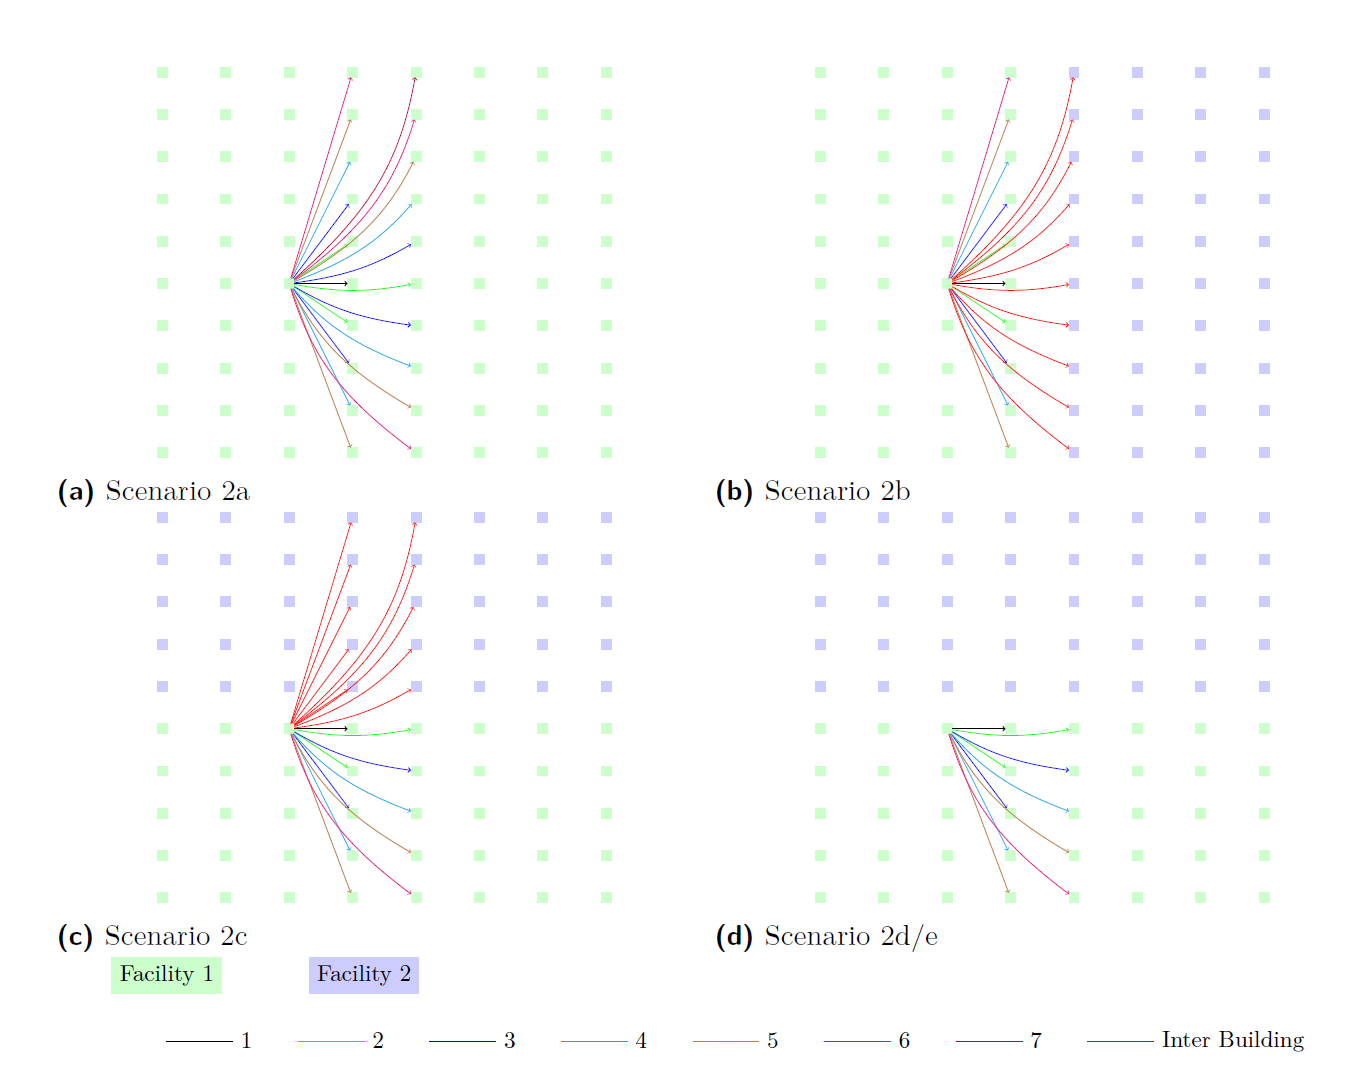
\includegraphics[width=8.8cm]{imagesjj/layoutalternatives}
\end{frame}


\begin{frame}
\frametitle{Five Scenarios Tested}
\begin{description}
\item[2a] Single facility organized in lanes

\item[2b] Two facilities in sequence (sequential for all jobs)

\item[2c] Two facilities in parallel with transport between facilities allowed

\item[2d] Two facilities in parallel, transport only within each facility

\item[2e] Two factories in parallel, with 80\% of jobs preassigned to a factory

\end{description}
\end{frame}

\begin{frame}
\frametitle{Scenario Comparison}
\begin{tabular}{l*{7}{r}}\toprule
       &   & \multicolumn{5}{c}{Scenario} & \\
Solver & Size  & 2a & 2b & 2c & 2d & 2e \\ \midrule
SICStus & 200  & \ccg 176.84& \ccg 184.84& \ccg 178.28& \ccg 180.52& \ccg 180.48 \\
\multicolumn{2}{l}{\% over Best}    &  0.00&  4.52&  0.81&  2.08\\
CPOptimizer & 200 & 184.40& 190.92& 186.00& 183.52& 183.52\\
\multicolumn{2}{l}{\% over Best}&  1.23&  4.81&  2.11&  0.75\\
Dispatch &200  & 182.76& 190.44& 184.28& 184.60& 184.64 \\
\multicolumn{2}{l}{\% over Best}&  0.00&  4.20&  0.83&  1.01\\
Local Search &200 & 184.68& 192.24& 185.76& 186.08& 185.96\\
\multicolumn{2}{l}{\% over Best}&  0.13&  4.23&  0.72&  0.89\\
\bottomrule
\end{tabular}

\end{frame}

\subsection{Summary}

\begin{frame}
\frametitle{Summary}
\begin{itemize}
\item New variant of known scheduling problem
\begin{itemize}
\item Arising from flexible new factory design

\item Transportation between machines/locations important element of schedule

\item Good solutions are obtained with CP for large problem instances

\item Not all CP models achieve the same solution quality
\item MIP results weak
\item Remaining, open gap between best lower bound and best solution found
\end{itemize}

\item Scheduling model used for factory design study
\begin{itemize}
\item Which layout gives the best overall results?
\item Explores four design alternatives
\end{itemize}

\end{itemize}
\end{frame}


\begin{frame}
\frametitle{Results Scale to Hundreds of Jobs (shown: SICStus 1000 jobs, 80 machines)}
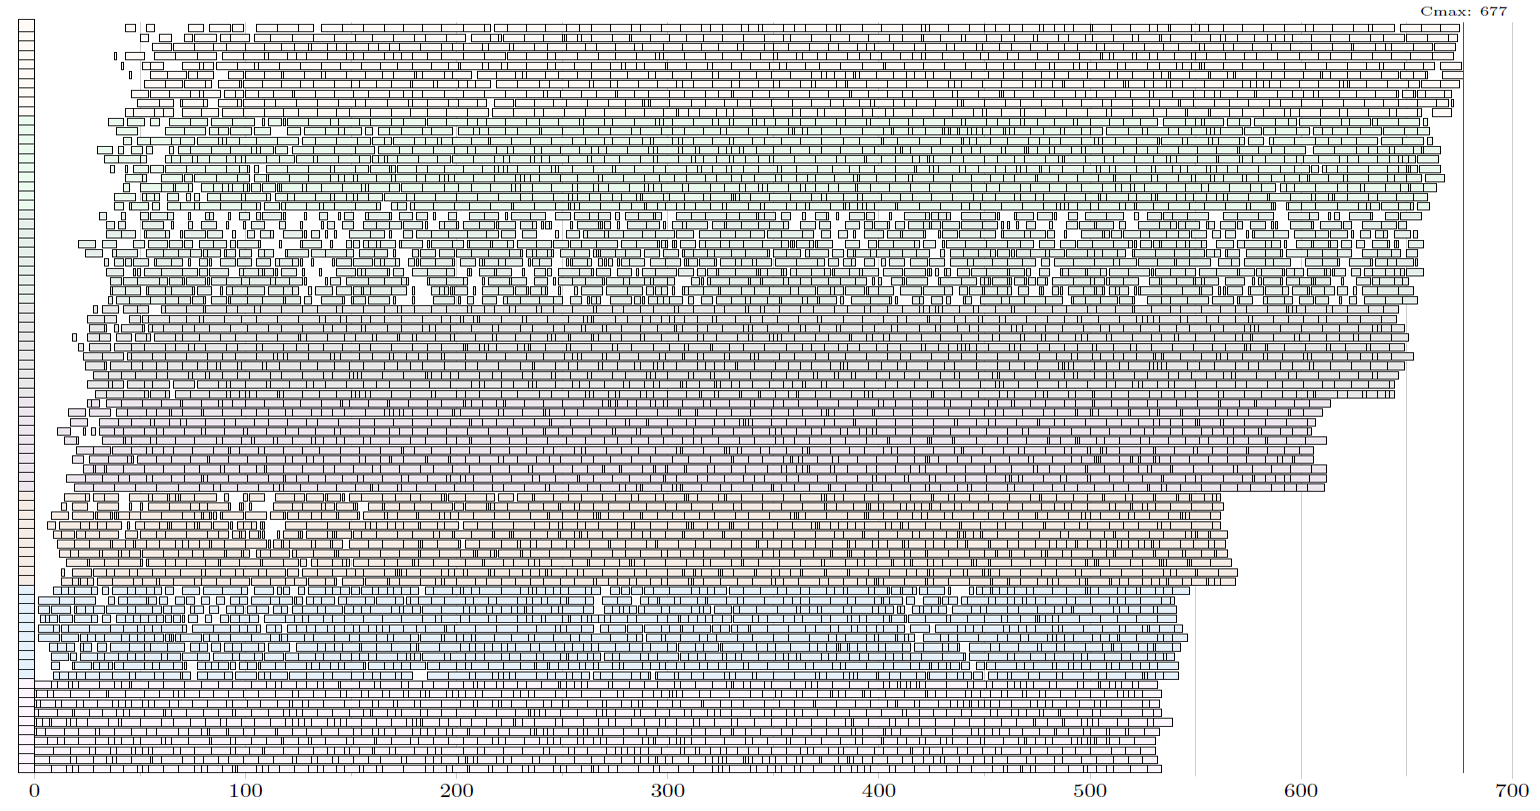
\includegraphics[width=14cm]{imagesjj/ganttchart}
\end{frame}







}
\mode<all>{\section{ASSISTANT SE Use Case}

\begin{frame}
\frametitle{An Industrial Example}
\begin{itemize}
\item ASSISTANT project Siemens Energy use case
\item Mid/Long-term scheduling/production planning
\item Realistic/not real data
\item Rather complex constraint model
\begin{itemize}
\item Multi-stage BOM
\item Alternative Process Paths
\item Alternative machines
\item Quality/cost based routing preferences
\item Potential outsourcing of certain steps
\item Machine specific calendars
\item Infeasible release/due date pairs
\item Calendar dependent speed reduction
\item Complex manpower constraints  
\end{itemize}
\end{itemize}
\end{frame}


\begin{frame}
\frametitle{Assistant Siemens Energy Use Case}
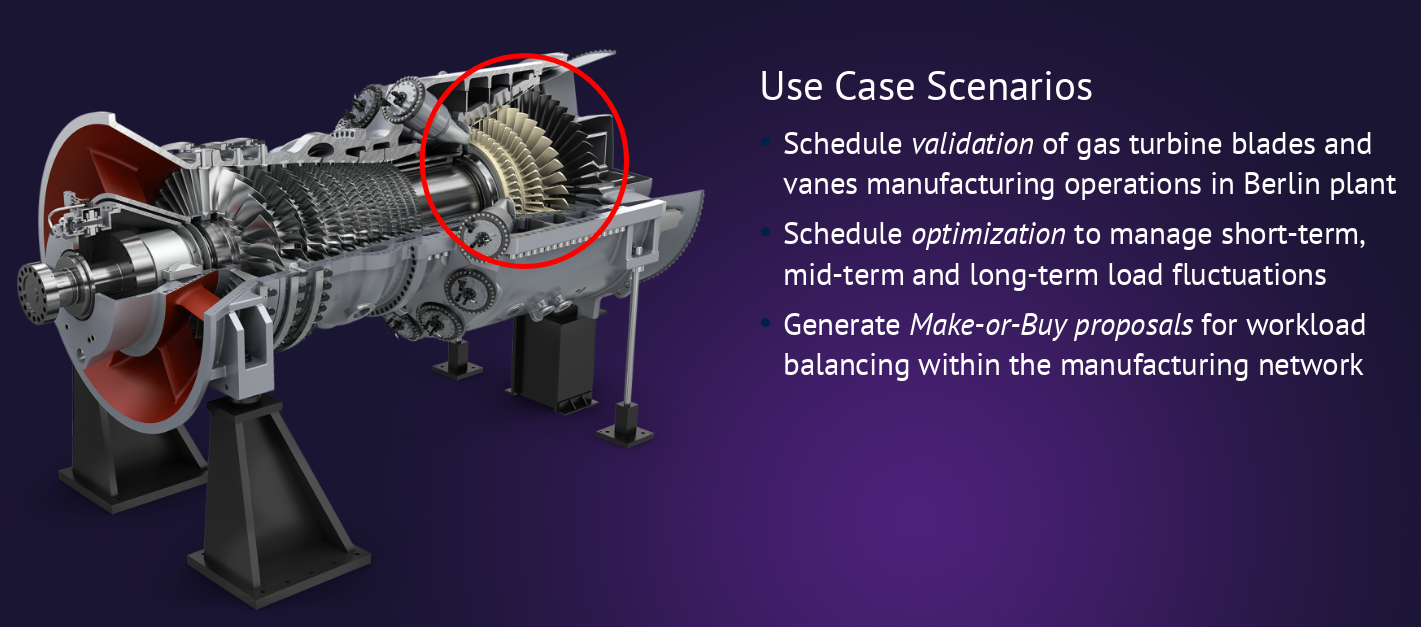
\includegraphics[width=\textwidth]{imagesse/assistantgasturbine}
\end{frame}

\begin{frame}
\frametitle{Digital Twin}
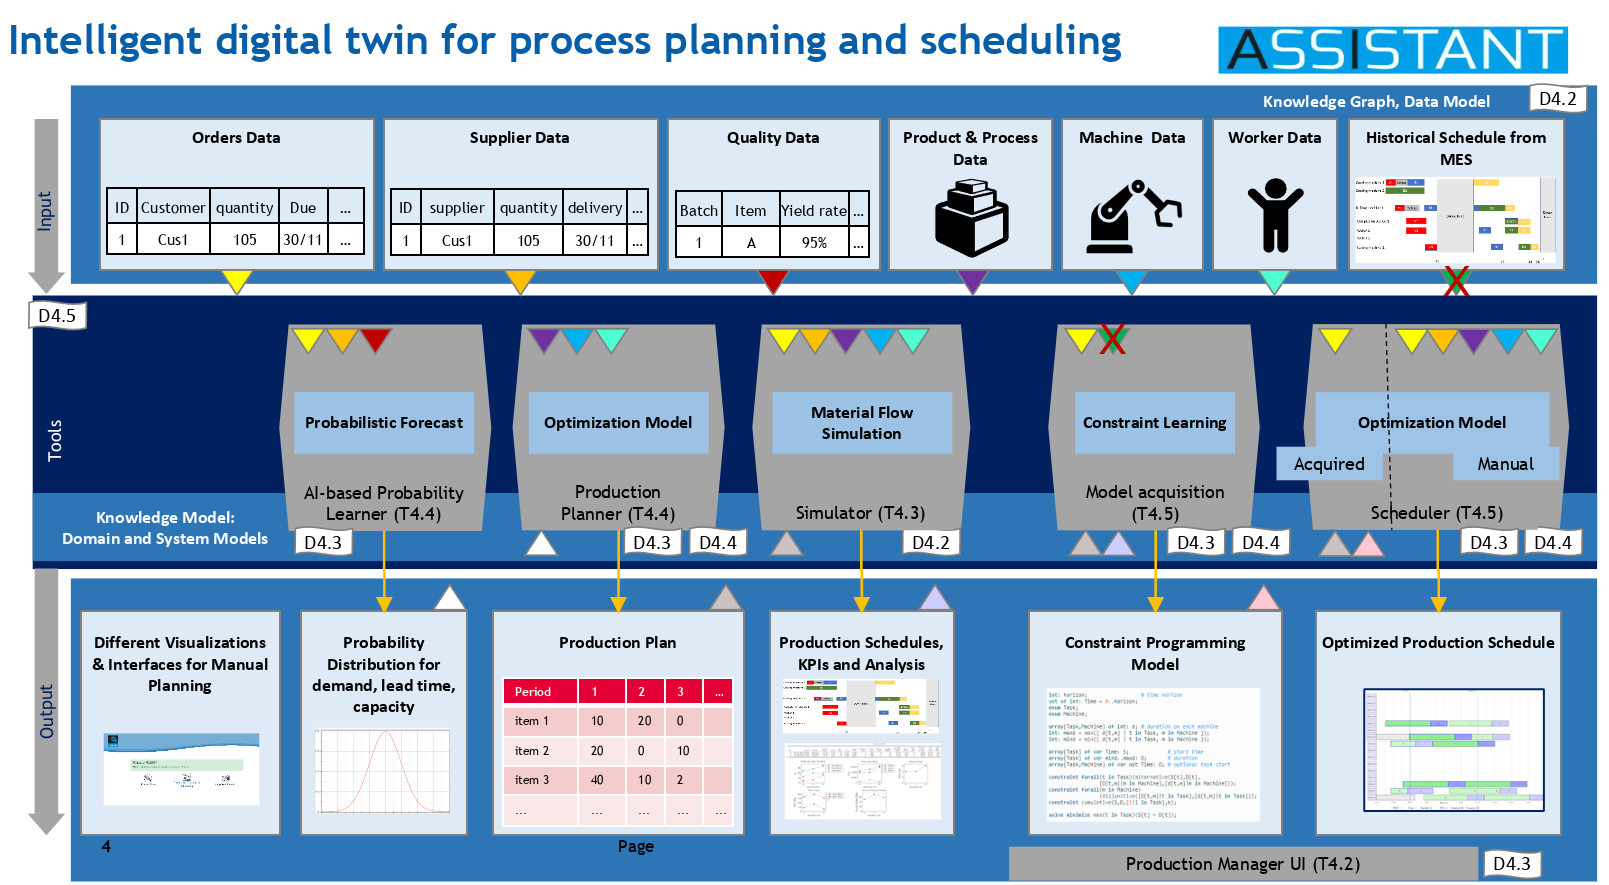
\includegraphics[width=.9\textwidth]{imagesse/assistantdigitaltwin}
\end{frame}

\begin{frame}
\frametitle{SE Product Routing}
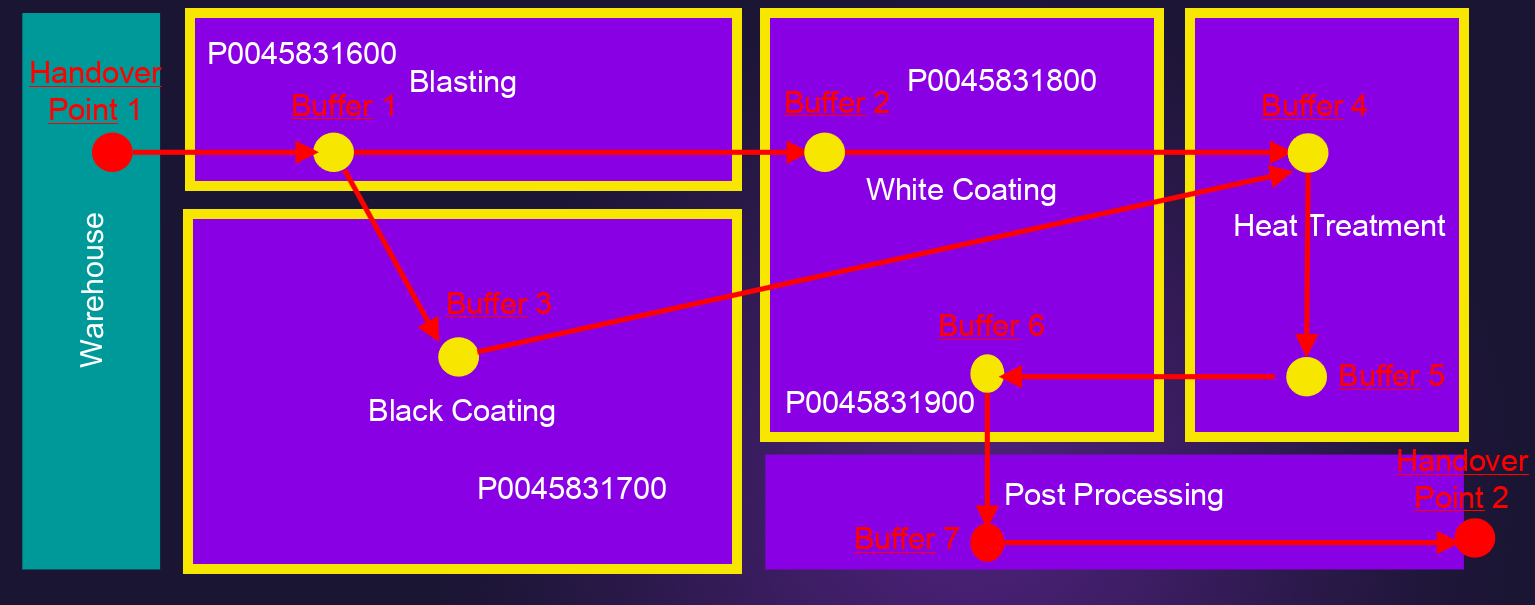
\includegraphics[width=\textwidth]{imagesse/assistantrouting}
\end{frame}

\begin{frame}
\frametitle{Datasets}
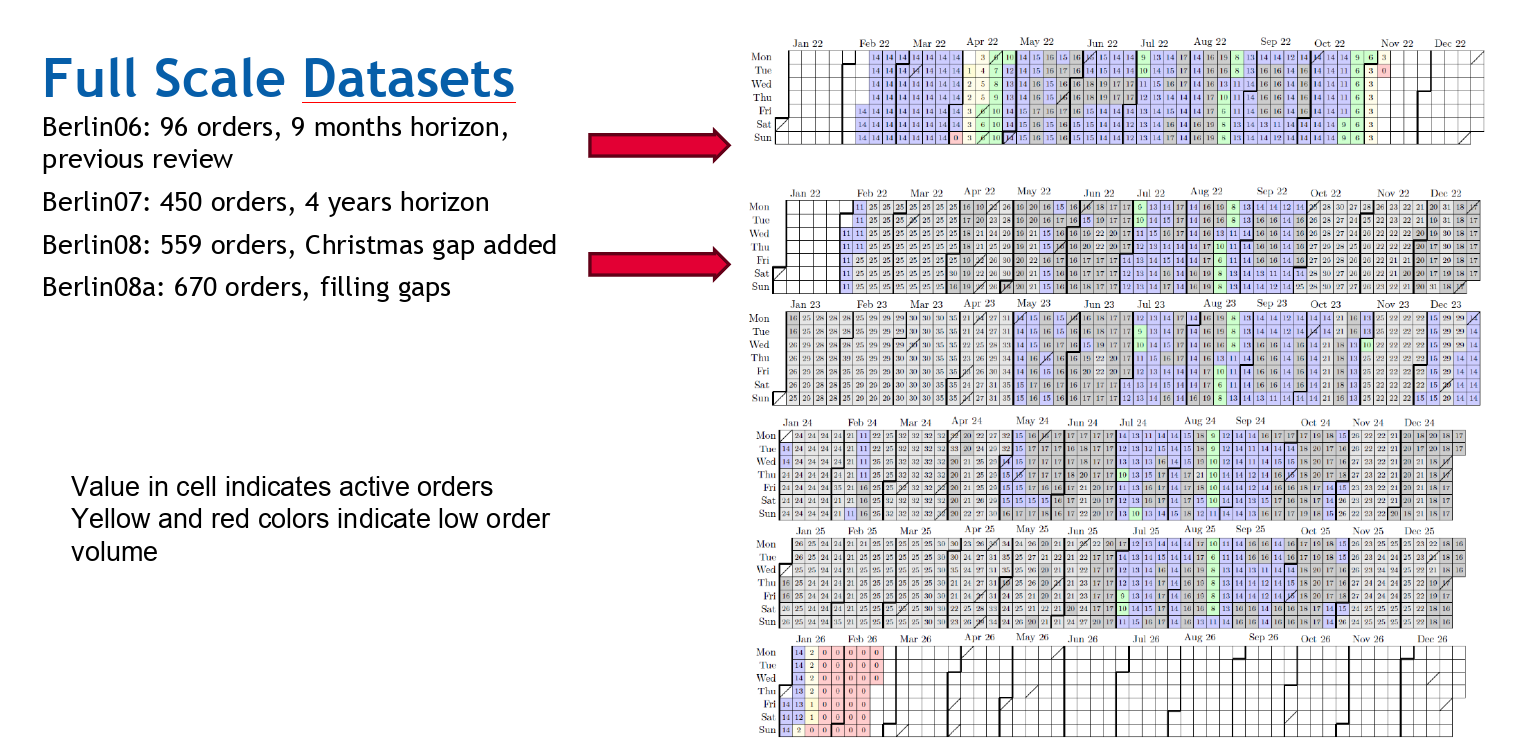
\includegraphics[width=\textwidth]{imagesse/assistantfullscaledatasets}
\end{frame}

\begin{frame}
\frametitle{Optimizer High Level Structure}
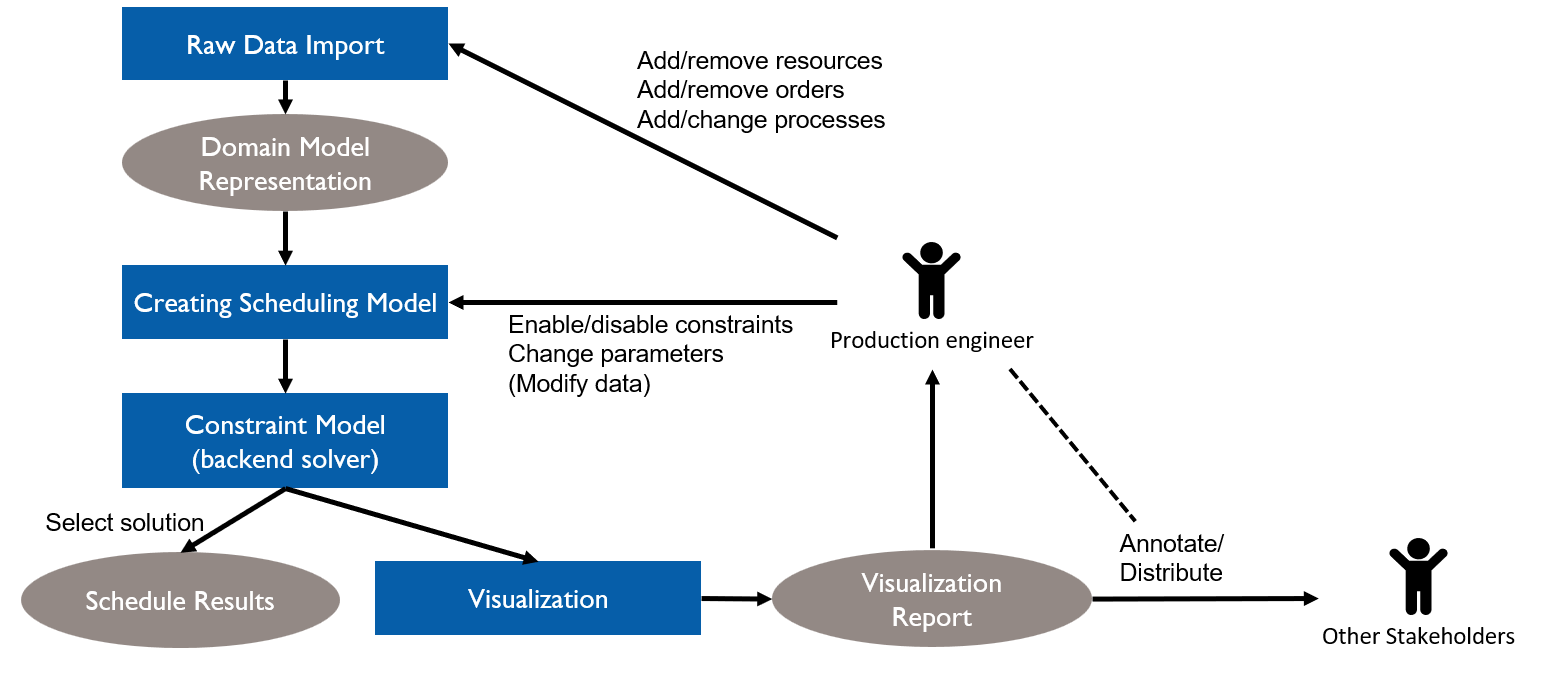
\includegraphics[width=.9\textwidth]{imagesse/overview}
\end{frame}

\begin{frame}
\frametitle{Raw Data - Manual Data Entry Causes Problems}
\begin{columns}
\begin{column}{0.5\textwidth}
\begin{itemize}
\item Raw data come from spreadsheet
\begin{itemize}
\item 20 tabs
\end{itemize}
\item Excel is a particularly bad input data format
\item Realistic, not real data
\item Created by hand/automatically from existing test scenarios
\item Series of files Berlin01 - Berlin05 were too inconsistent to run
\item Berlin06 still contains some errors
\item Optimizer explains all issues that it finds
\end{itemize}
\end{column}
\begin{column}{0.5\textwidth}
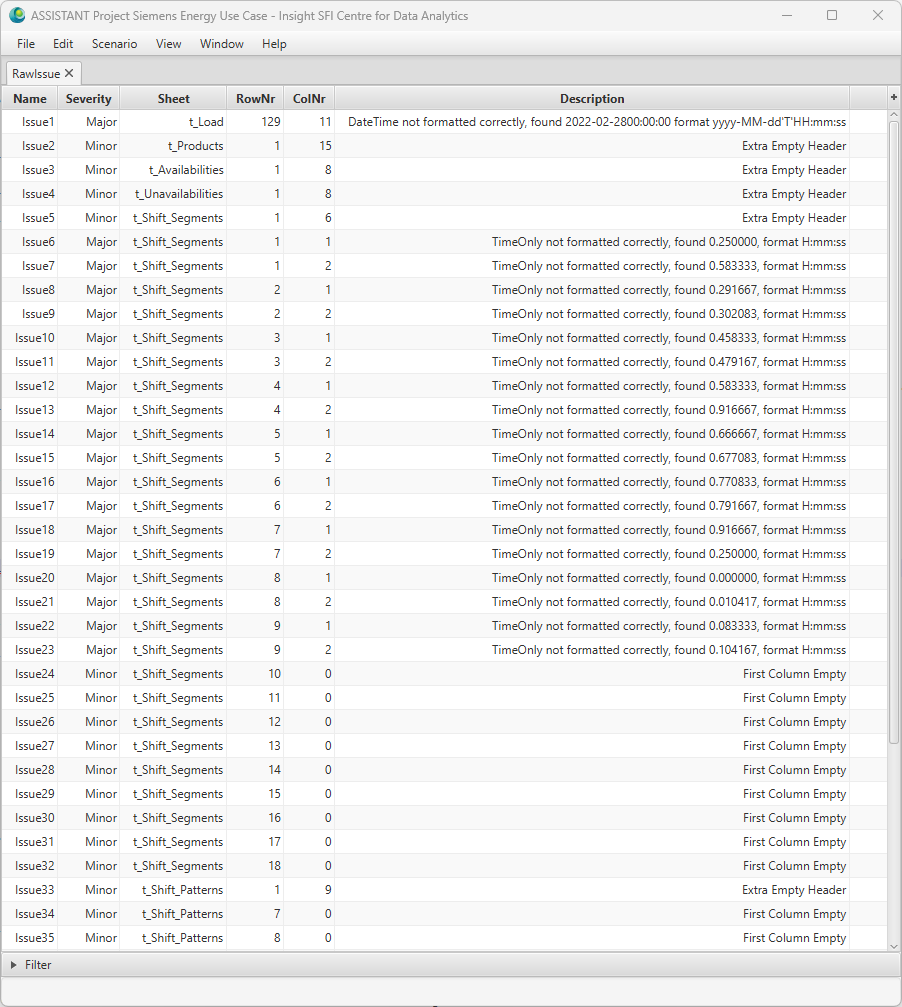
\includegraphics[width=.85\textwidth]{imagesse/rawerror}
\end{column}
\end{columns}
\end{frame}

\begin{frame}
\frametitle{Domain Model - Knowledge Graph}
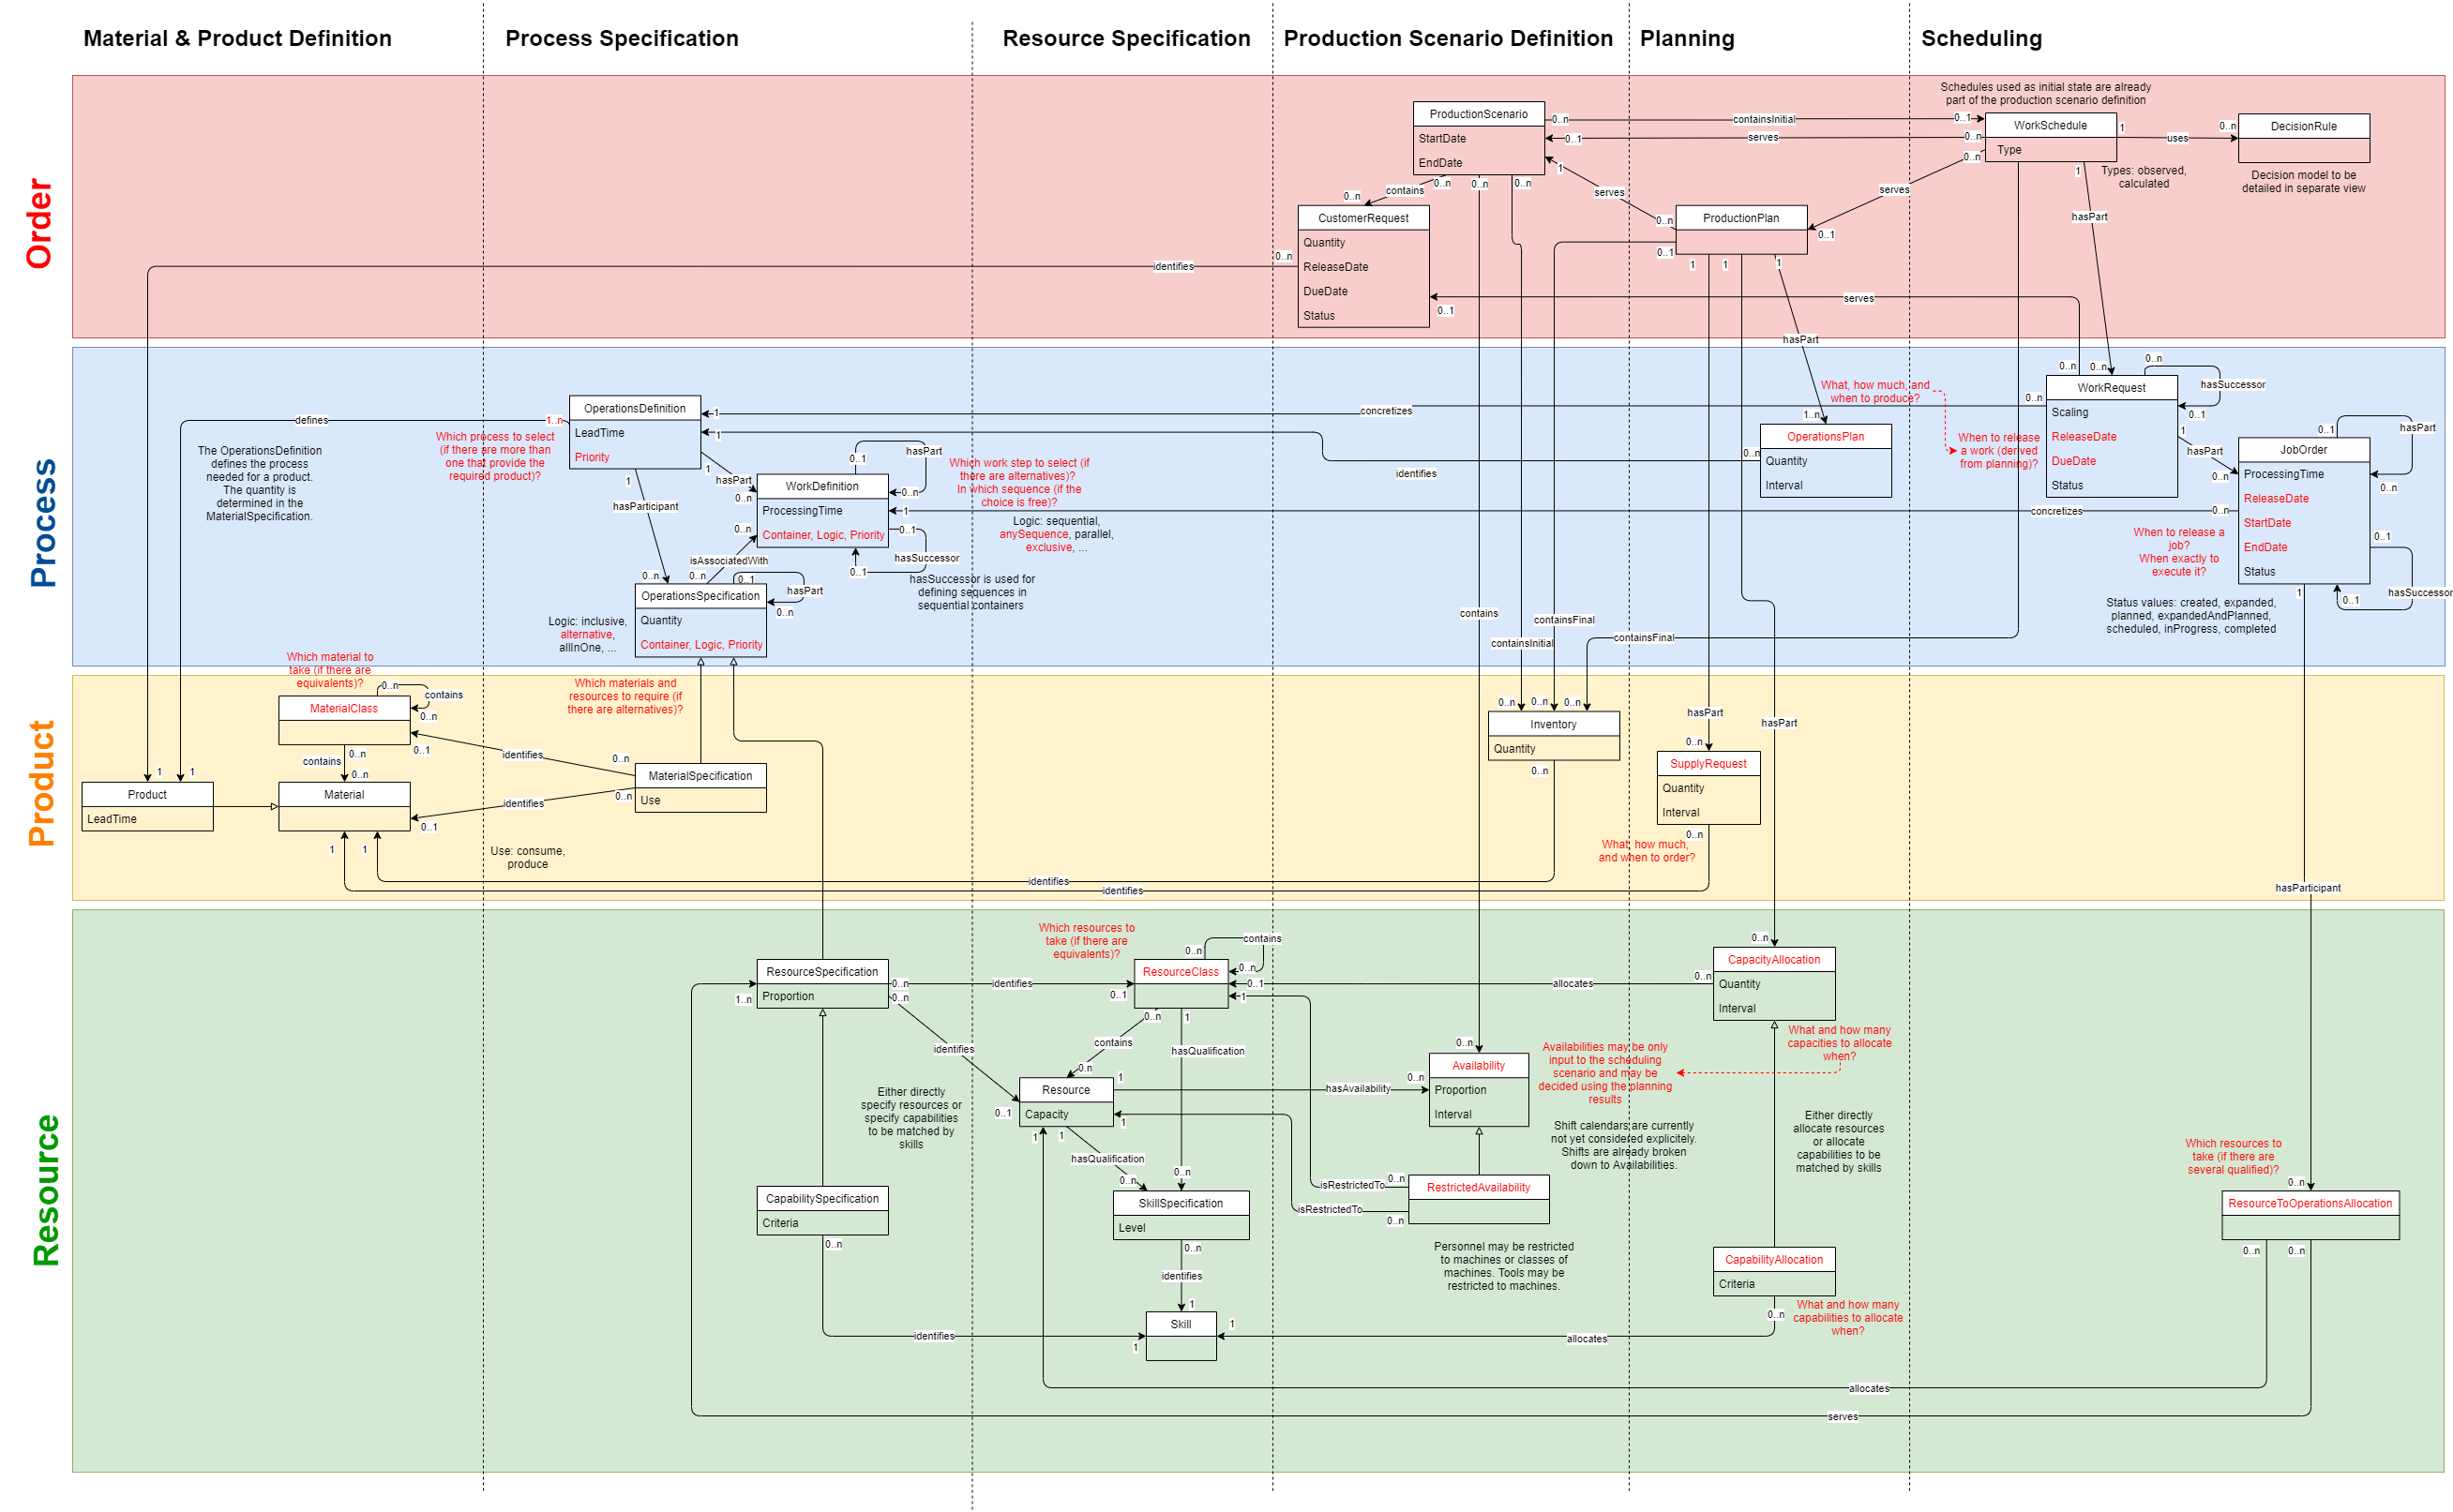
\includegraphics[width=.8\textwidth]{imagesse/DomainModel}
\end{frame}

\begin{frame}
\frametitle{Single Solution for Berlin 08a - Shows Only 20\% of Tasks in Model}
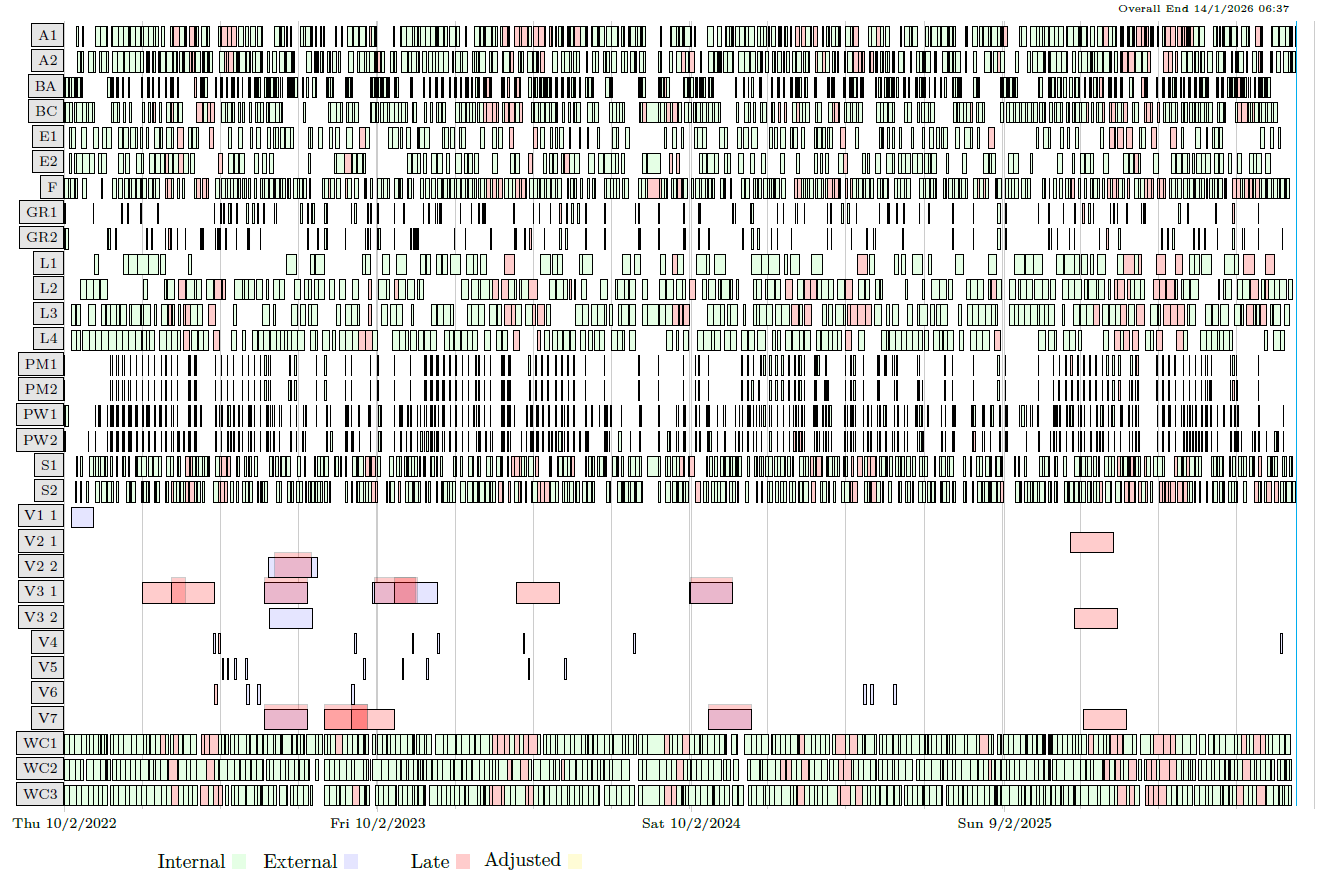
\includegraphics[width=.75\textwidth]{imagesse/solution08apref2}
\end{frame}

\begin{frame}
\frametitle{Implementation}
\begin{itemize}
\item Requirement capture done inside project
\item Data checking/cleaning most time consuming aspect
\item Some specified functionality was rejected by Betriebsrat
\item Built in Java
\item Uses IBM's CPO back-end
\item 120k LoC, 110k generated, 3k solver
\item Outperforms both 
\begin{itemize}
\item Current in-house tool
\item Simulation based tool based on commercial simulator 
\end{itemize}
\item System installed at SE site, but not in daily use
\end{itemize}
\end{frame}


\begin{frame}
\frametitle{CPO Keeps on Trucking}
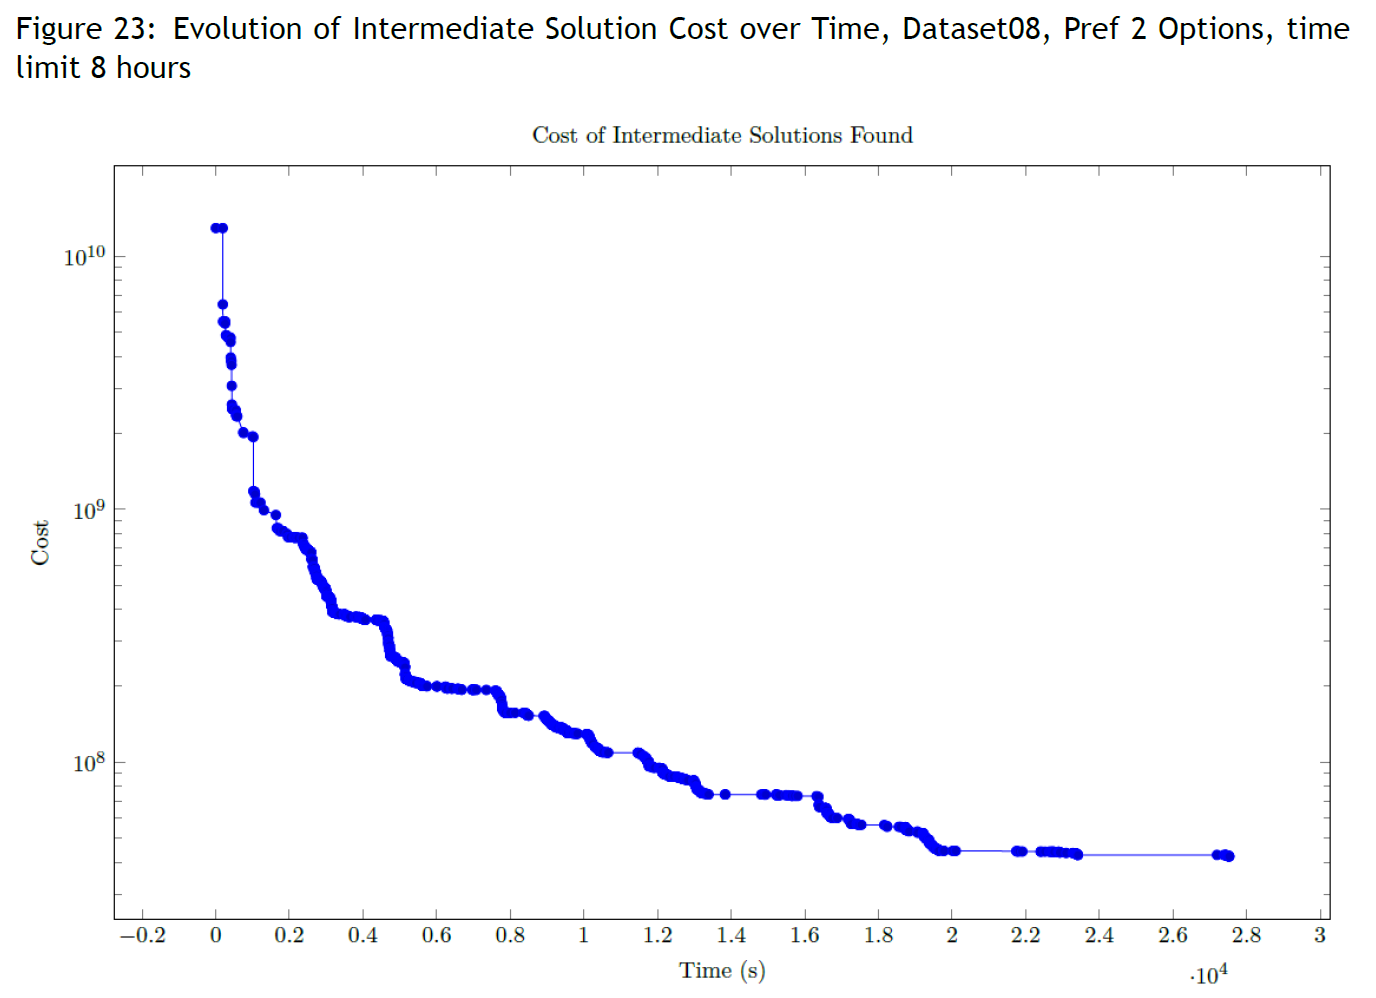
\includegraphics[width=.65\textwidth]{imagesse/improving}
\end{frame}

\begin{frame}
\frametitle{Conclusion}
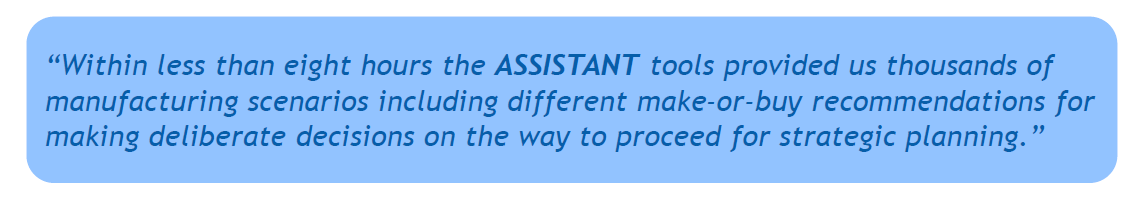
\includegraphics[width=.9\textwidth]{imagesse/quote}

{\tiny Siemens SE final project review assessment}
\end{frame}



}
\mode<all>{\section{Outpatient Waitlist Management}


\begin{frame}
\frametitle{Joint work with...}
\begin{itemize}
\item Mike O'Keeffe
\item Adrian O'Leary
\item Barry O'Sullivan
\item At Insight Centre for Data Analytics, University College Cork
\end{itemize}
\end{frame}

\subsection{Introduction}

\begin{frame}
\frametitle{Real-World Problem}
\begin{itemize}
\item Healthcare in Ireland
\item Wait times for patients are out of control, even before Covid-19
\item Longer wait times, poorer patient outcomes
\item Critical to understand where to invest
\item Currently: no tools to understand how changes affect performance
\end{itemize}
\end{frame}

\begin{frame}
\frametitle{Research Challenges}
\begin{itemize}
\item How to model hospital environment, many independent actors
\item Deal with uncertain demand, and uncertain outcomes
\item Understand where capacity is lost/not used
\end{itemize}
\end{frame}

% \begin{frame}
% \frametitle{Take-Away Message}
% \begin{itemize}
% \item Irish hospitals are in deep crisis
% \item Decision analytics can help to understand and solve problems
% \item Optimization key aspect of solving problem
% \item Very hard to affect change
% \item Stakeholder factors much more complex than in industry 
% \end{itemize}
% \end{frame}

% \begin{frame}
% \frametitle{Ireland Background}
% \begin{tabular}{ccc}
% 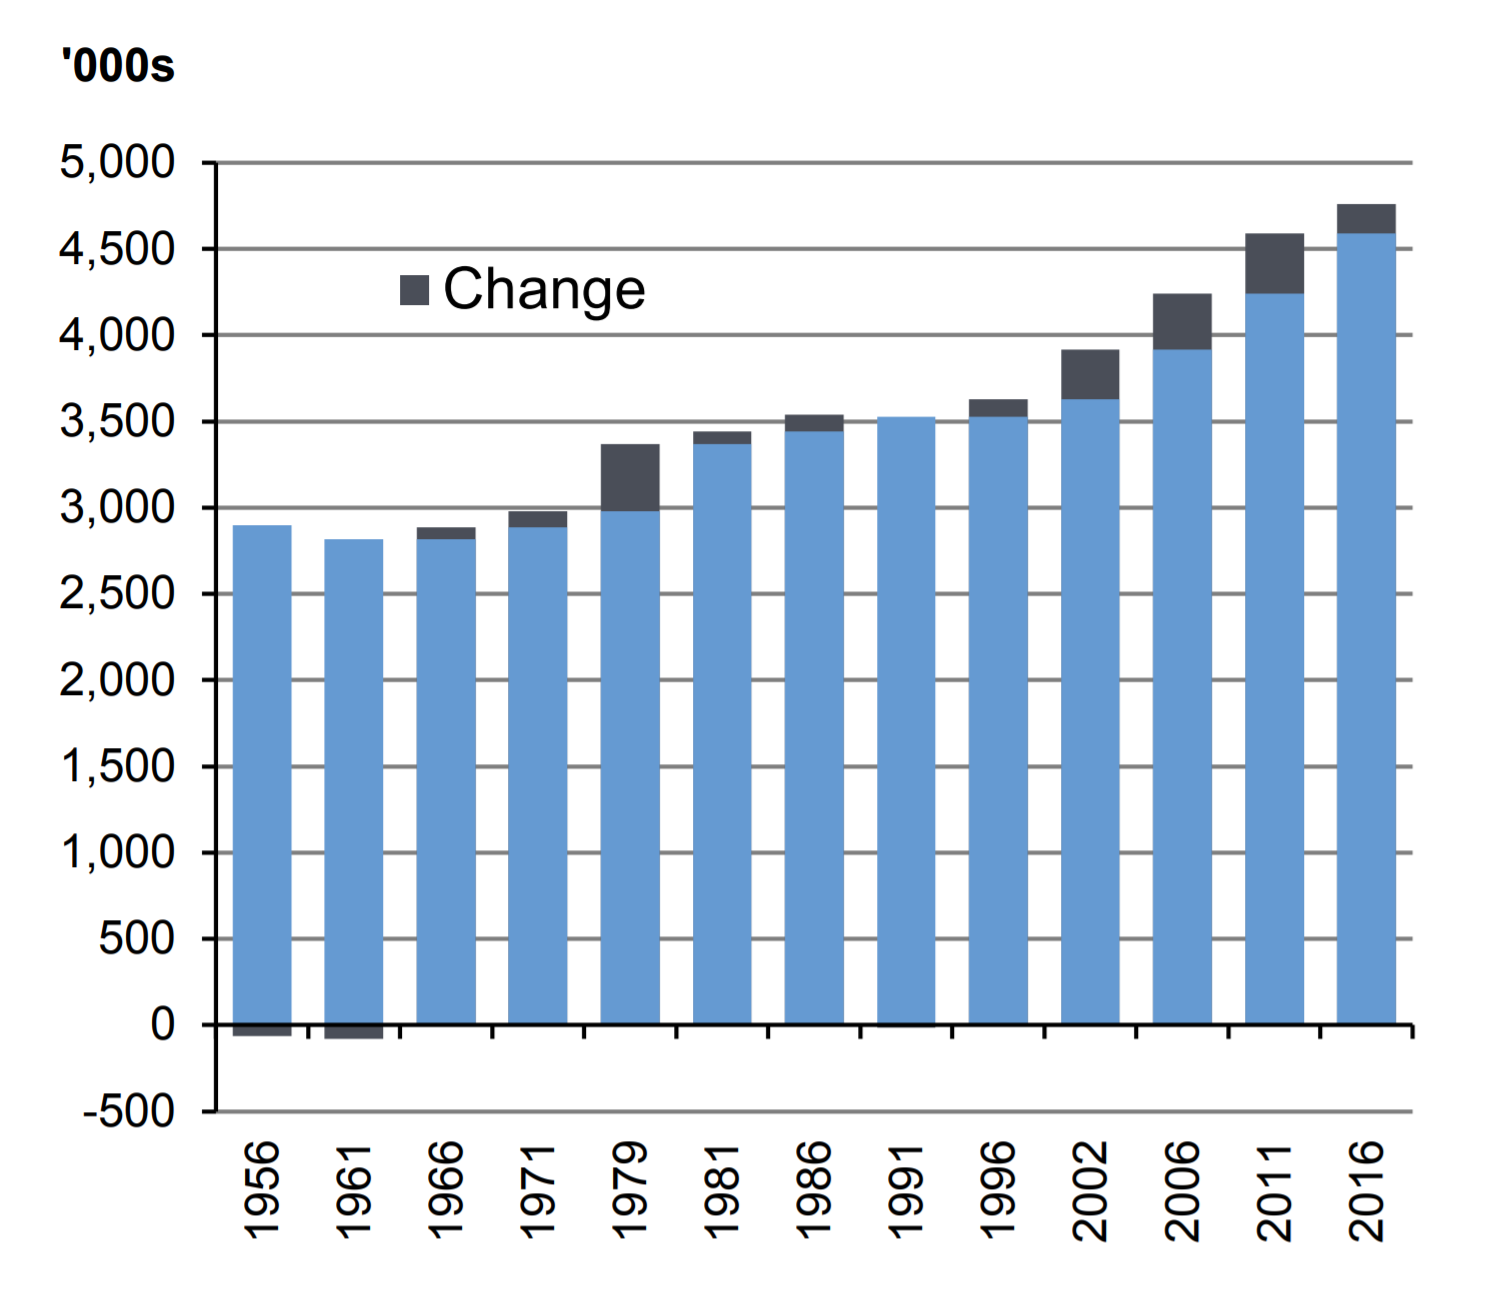
\includegraphics[width=3.5cm]{imagesoutpatient/census}
% &
% 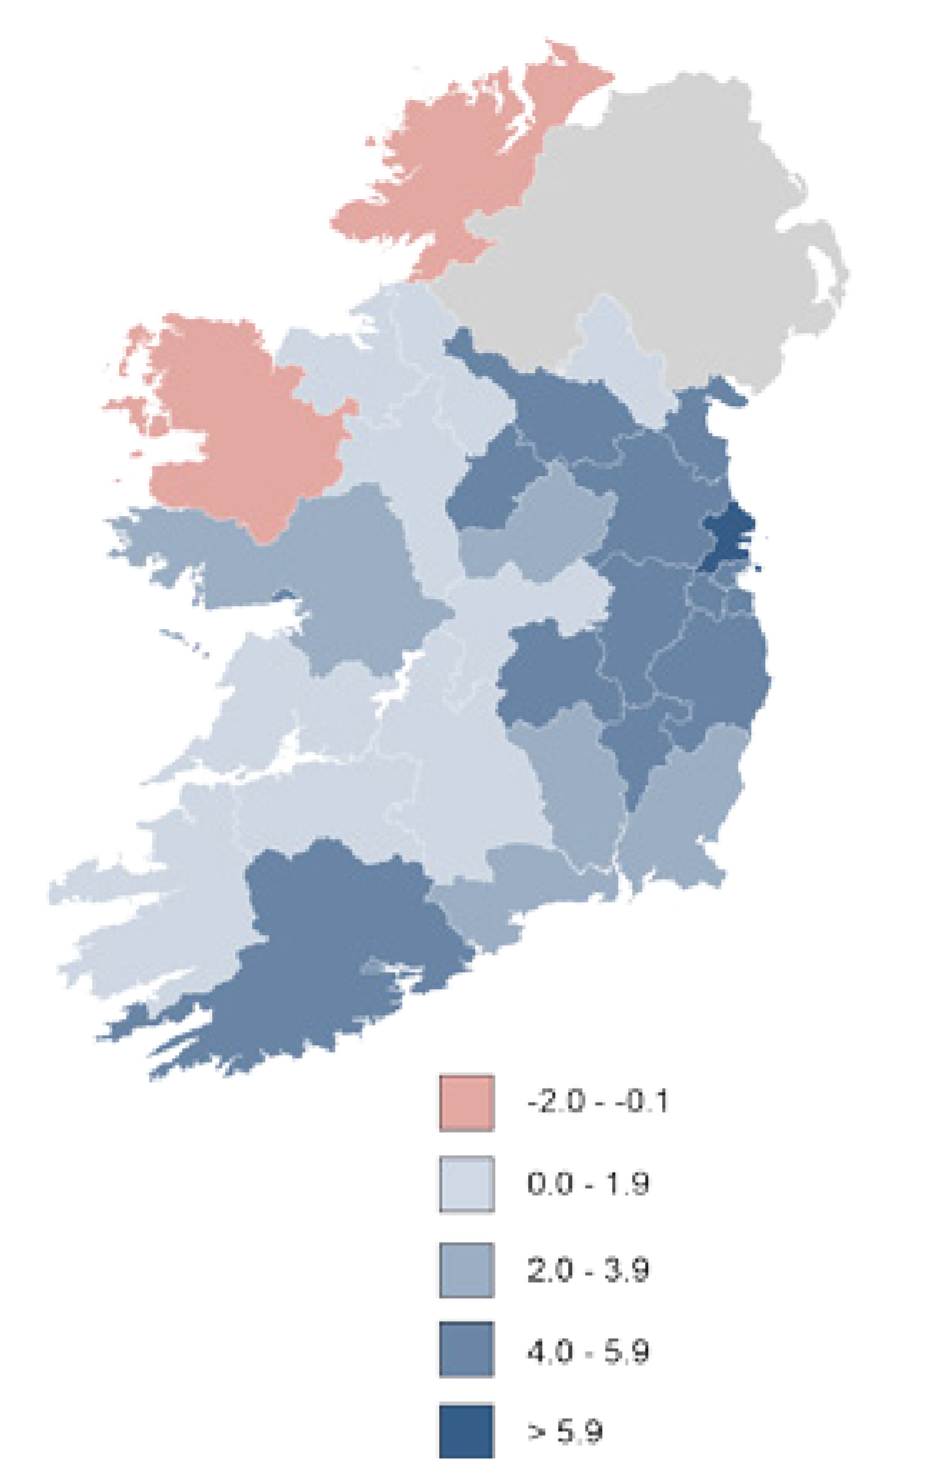
\includegraphics[width=3.5cm]{imagesoutpatient/populationchangebycounty}
% &
% 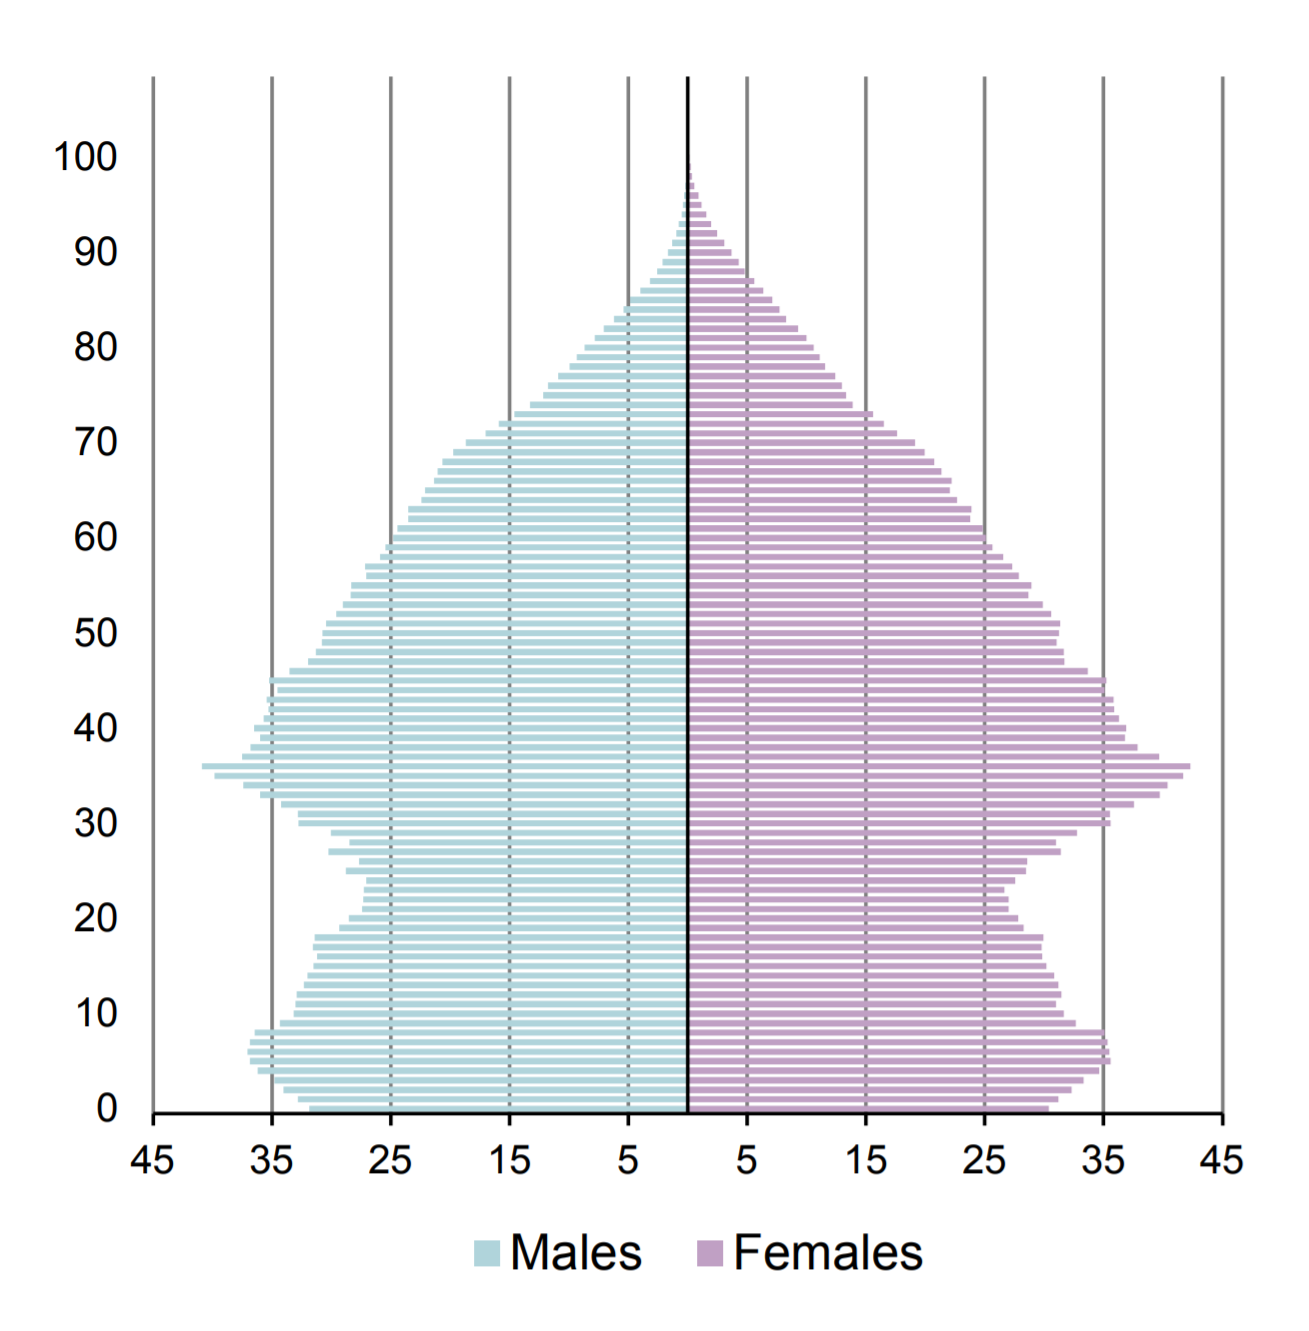
\includegraphics[width=3.5cm]{imagesoutpatient/populationtree}
% \\
% \shortstack{Population\\Over Time}
% &
% \shortstack{Population\\Change\\By County}
% &
% \shortstack{Age Distribution\\by Sex}
% \end{tabular}

% {\scriptsize Source: Census 2016, CSO}
% \end{frame}


% \begin{frame}
% \frametitle{Health Care in Ireland}
% \begin{tabular}{cc}
% 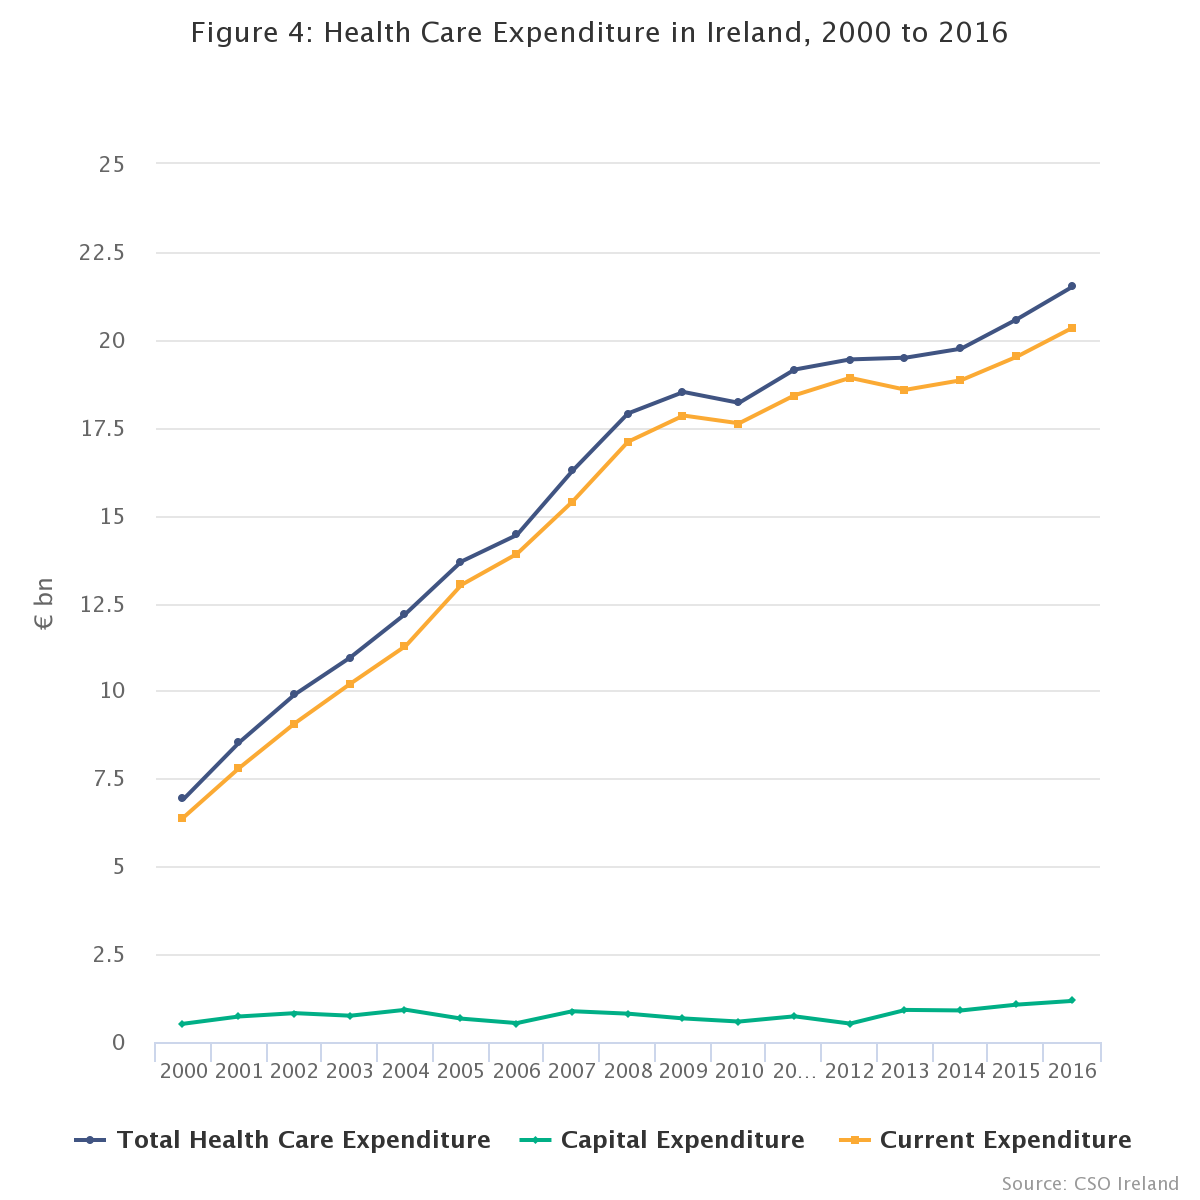
\includegraphics[width=5cm]{imagesoutpatient/healthcareexpenditure}
% &
% 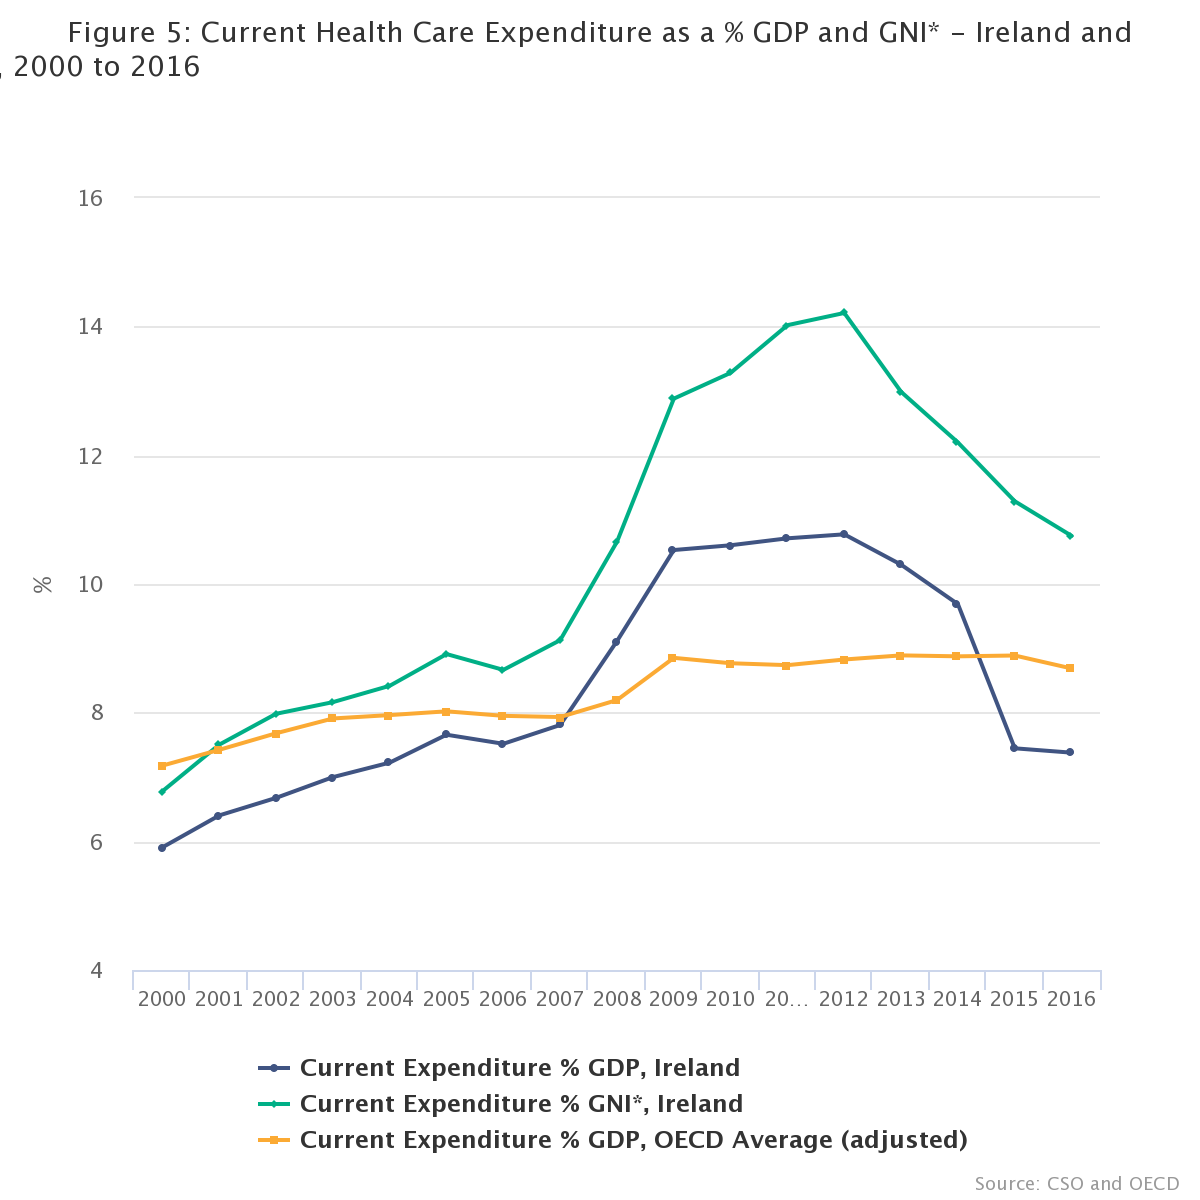
\includegraphics[width=5cm]{imagesoutpatient/healthcareaspartofgnp}\\
% Total Spend & As Percent of GDP/GNI\\
% \end{tabular}

% \vspace{0.5cm}
% {\scriptsize Source: System of Health Accounts 2016, CSO}
% \end{frame}

% \begin{frame}
% \frametitle{Compared to Other Countries (2017)}
% 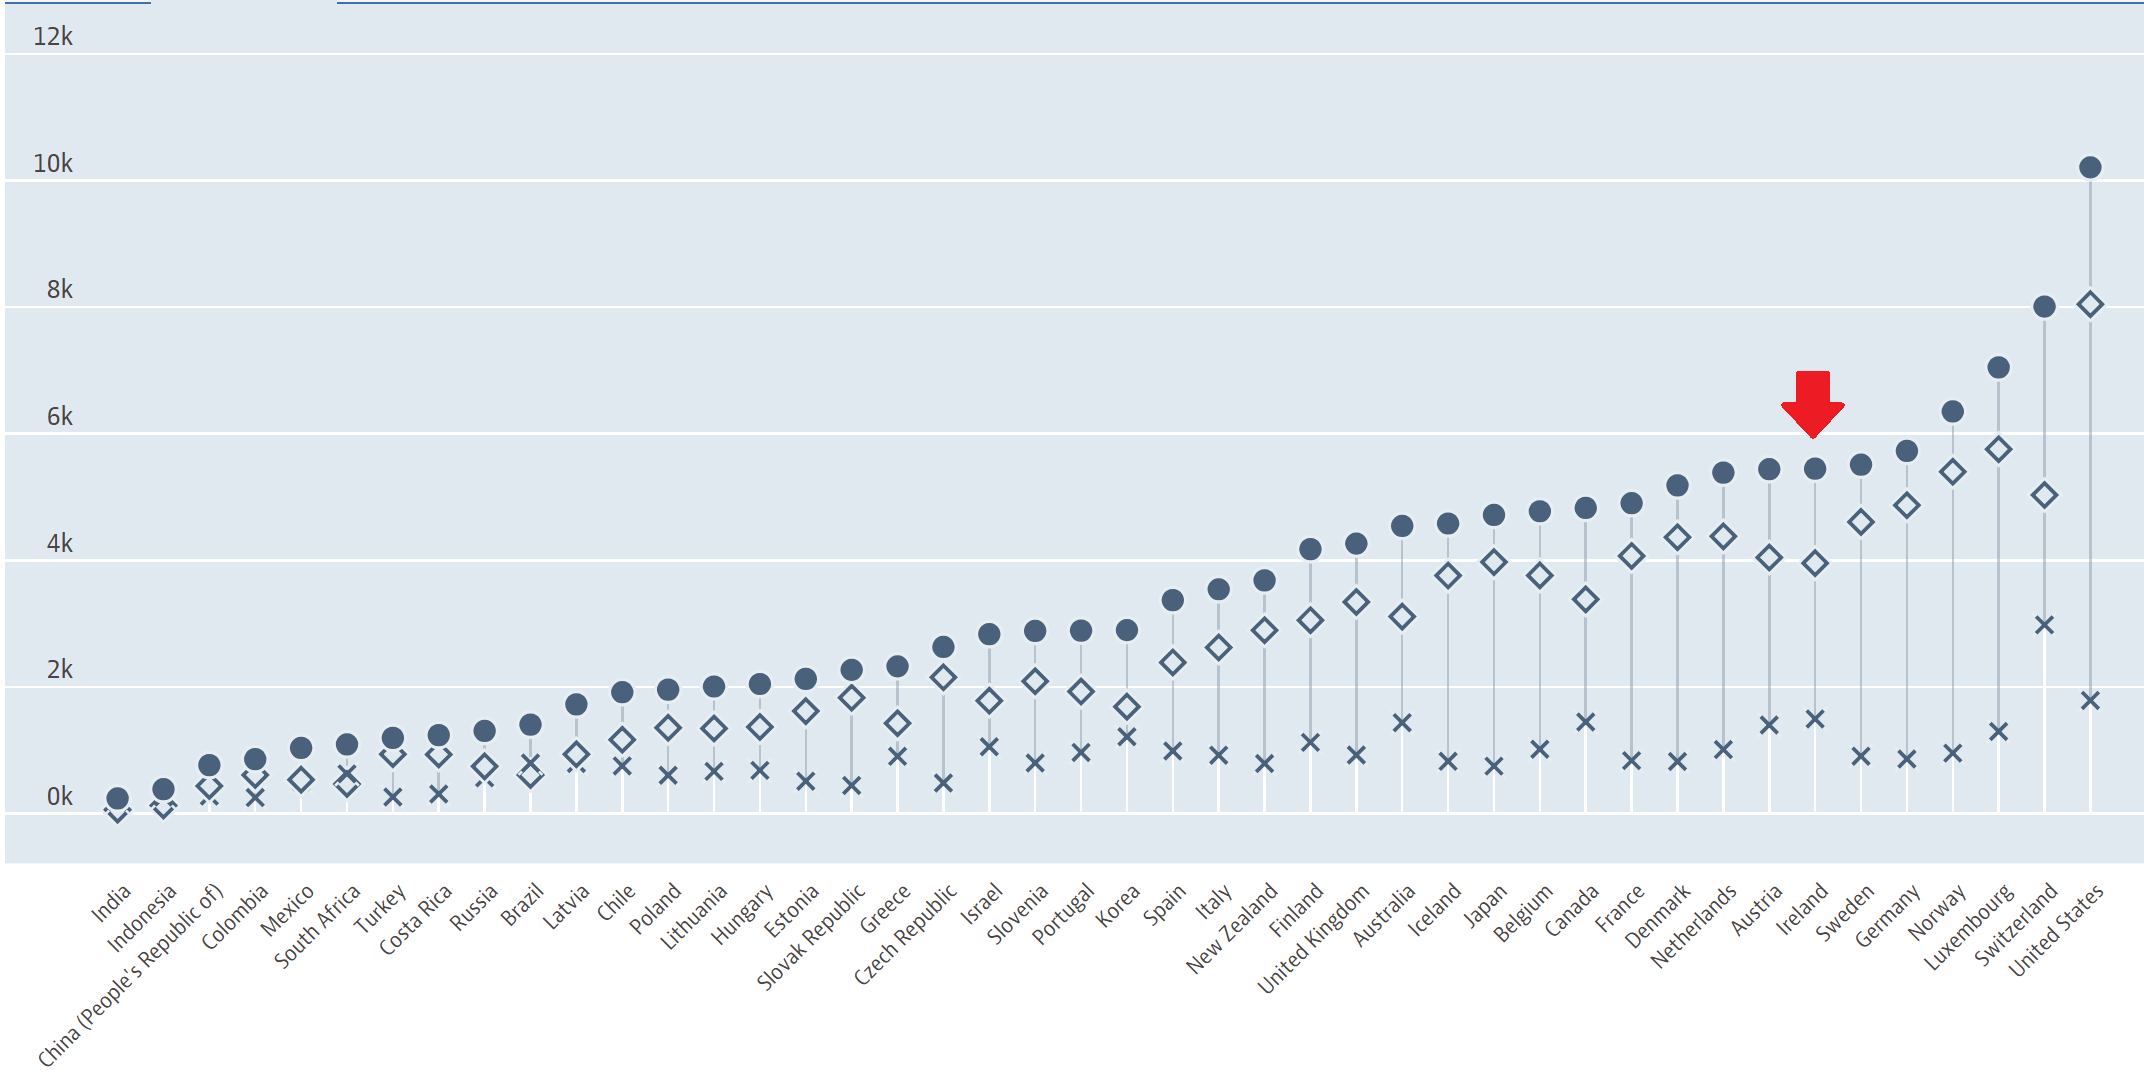
\includegraphics[width=11cm]{imagesoutpatient/oecdhealthspending}

% \vspace{0.5cm}
% {\scriptsize Source: OECD, Health Care Spend per Capita in PPP USD}
% \end{frame}



%% \begin{frame}
%% \frametitle{Hospital Groups}
%% 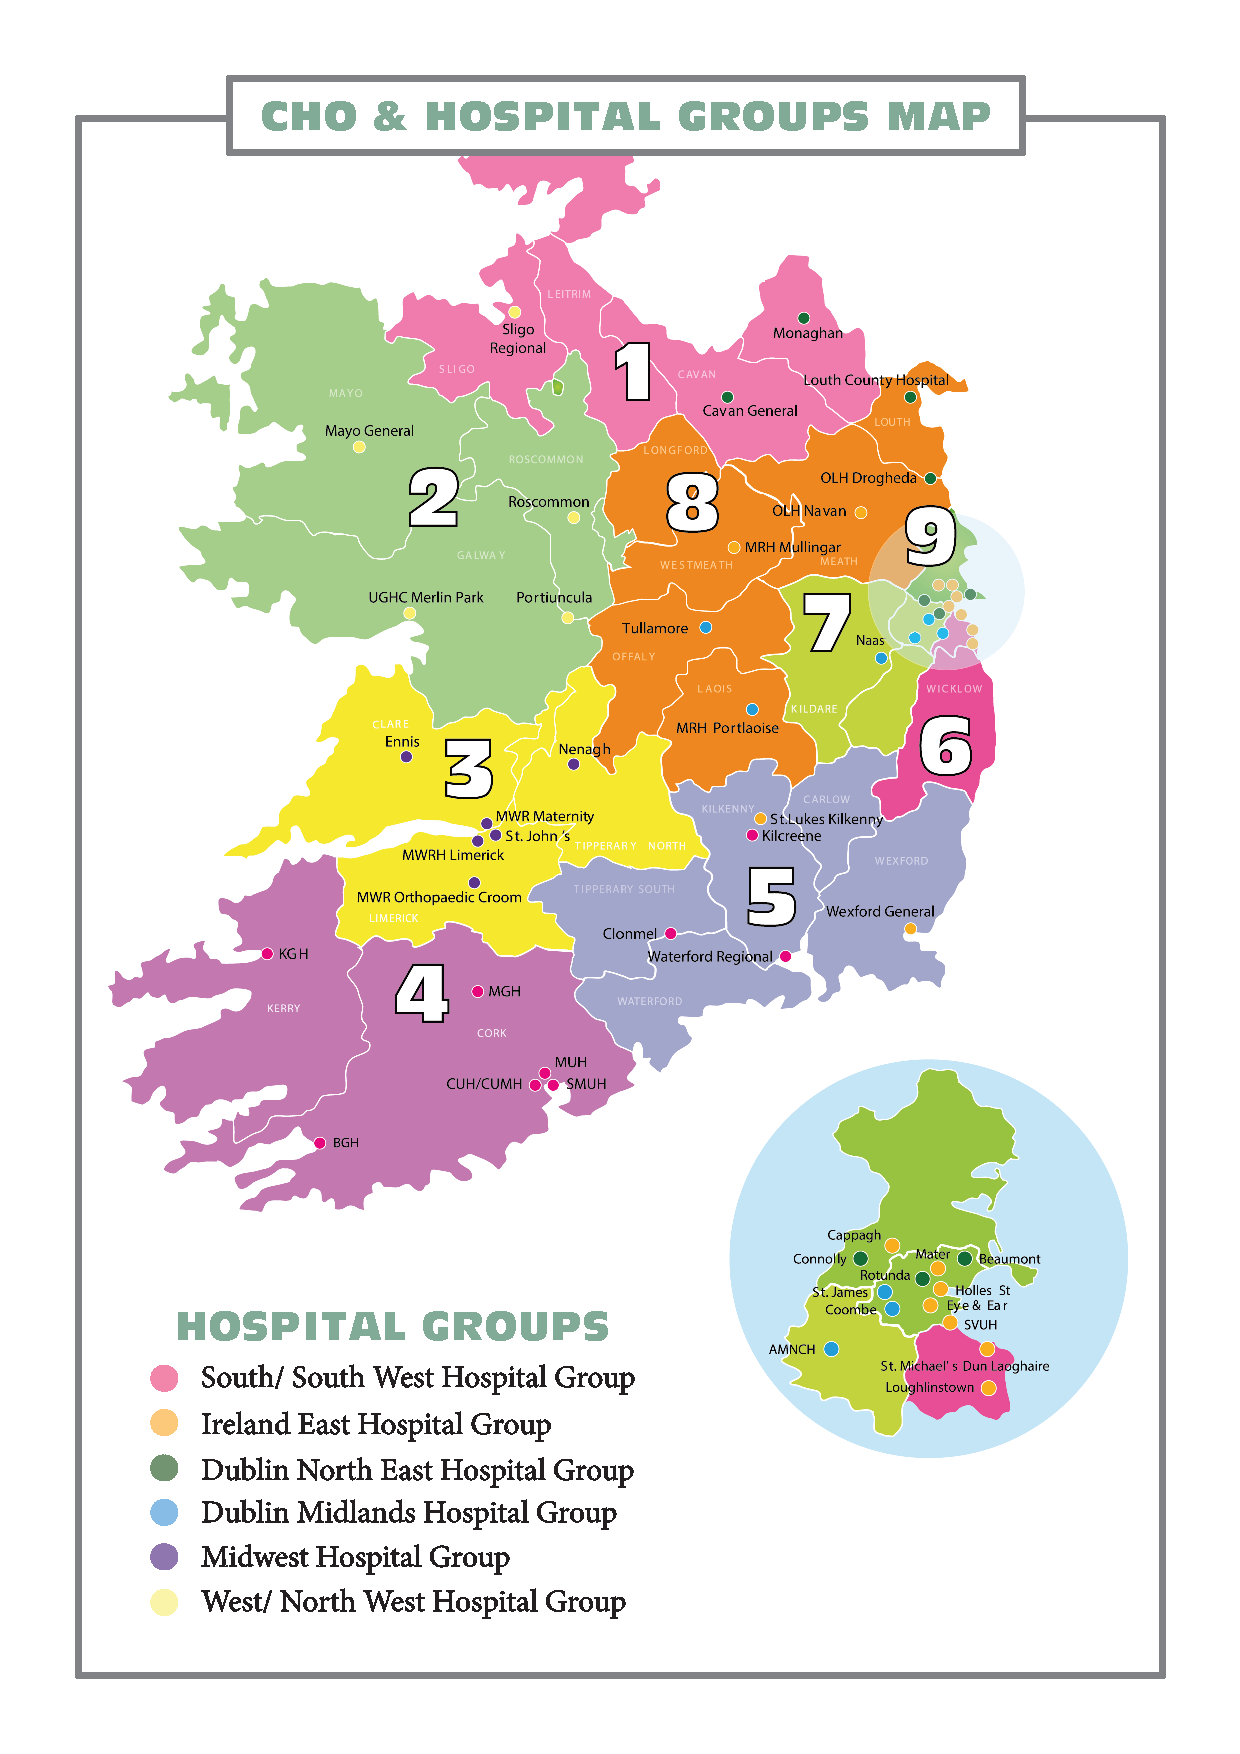
\includegraphics[width=5cm]{imagesoutpatient/cho-area-map-with-hospital-groups}
%% \end{frame}

\begin{frame}
\frametitle{Hospital Services Overview}
%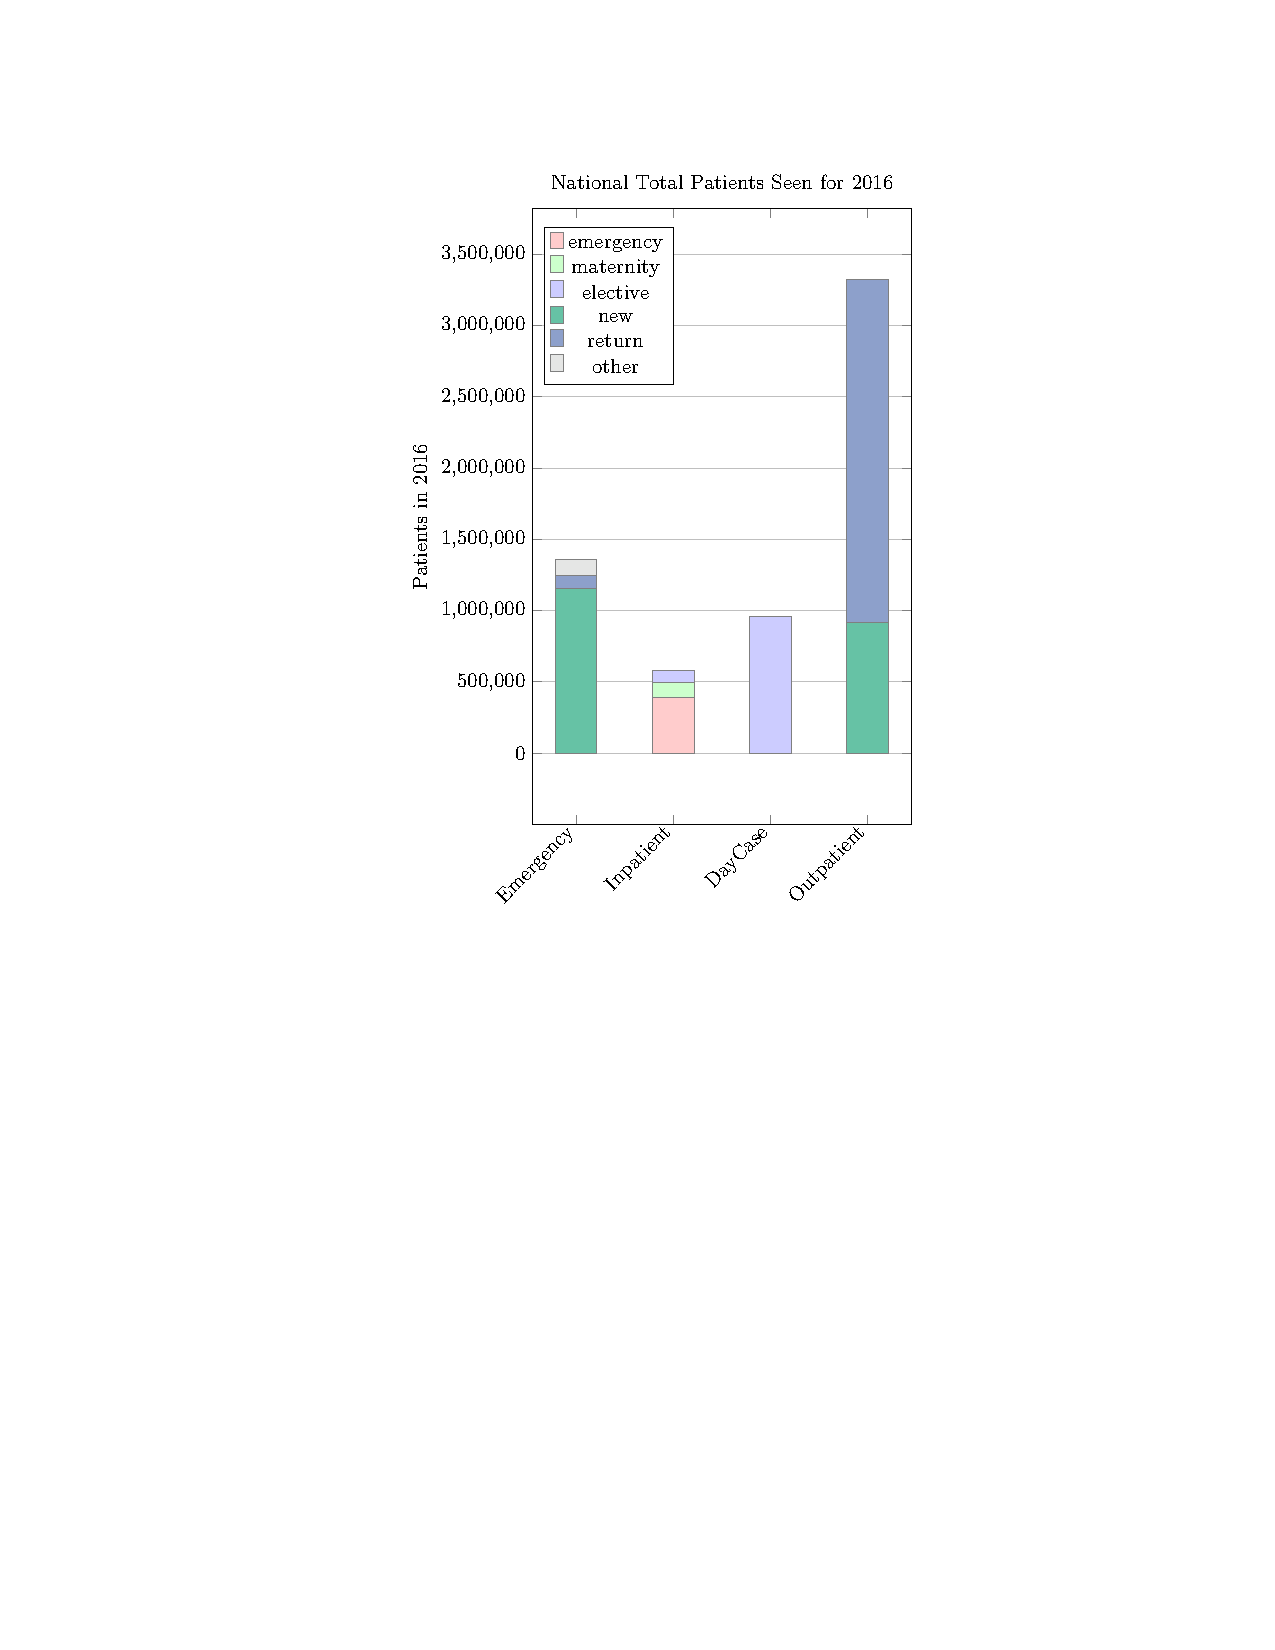
\includegraphics[width=11cm]{imagesoutpatient/patienttypes}
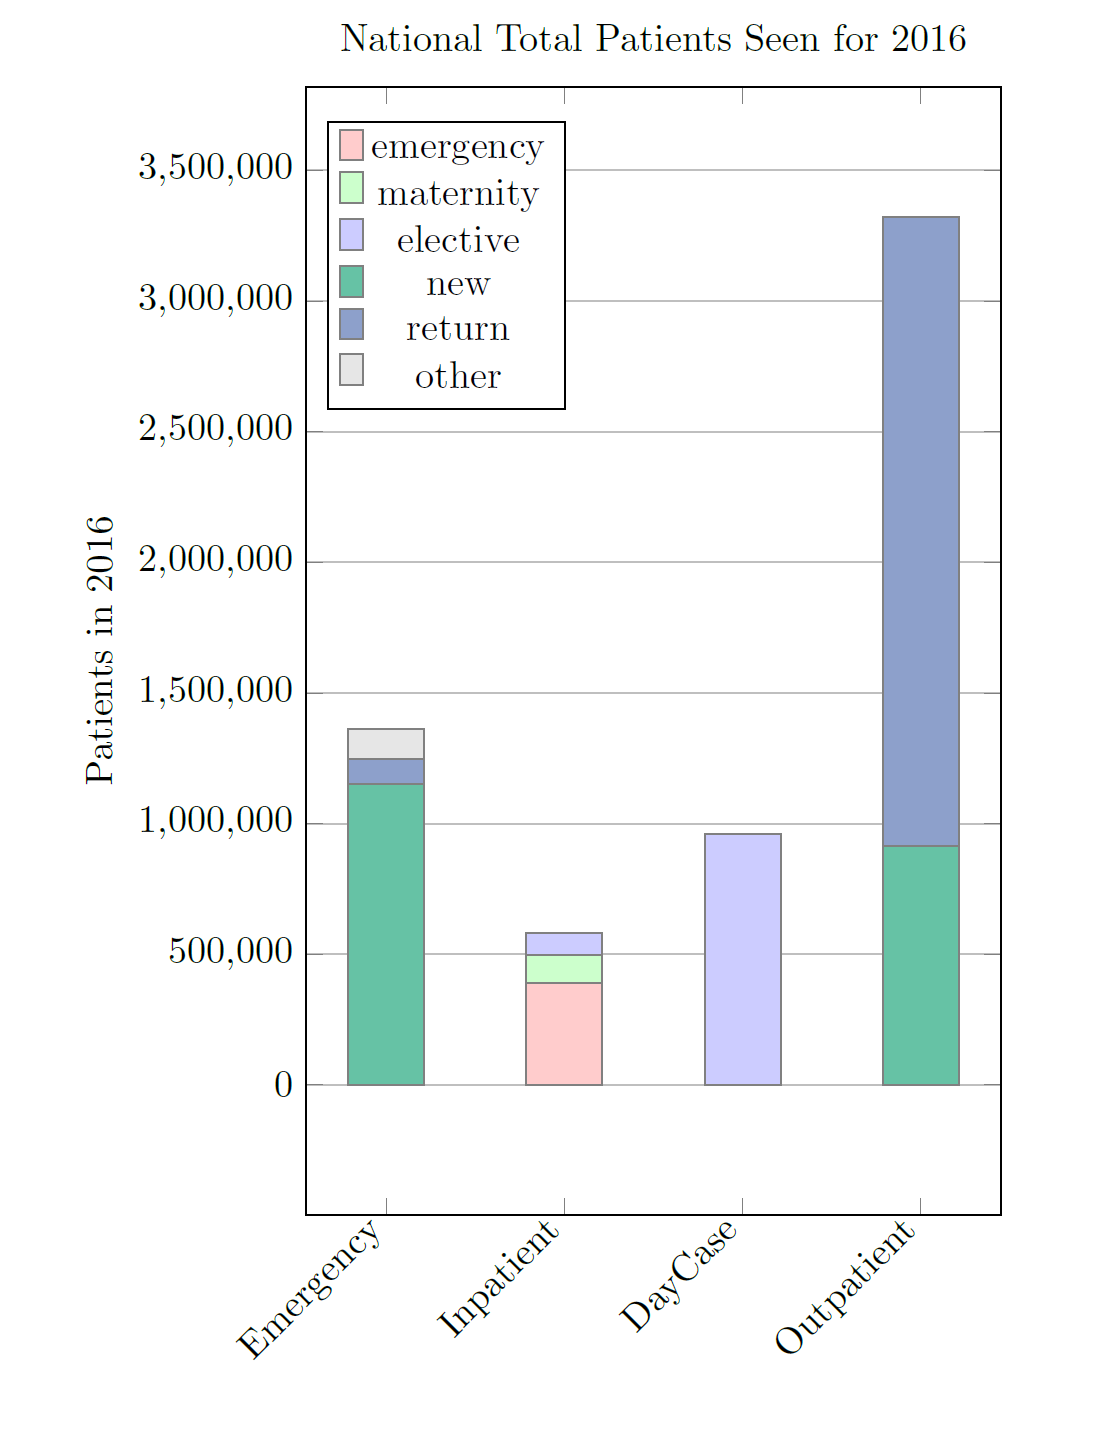
\includegraphics[width=5.5cm]{imagesoutpatient/patienttypes2016}
{\scriptsize \shortstack{Data: HSE Management Data Report, Dec 2016}}
\end{frame}

\begin{frame}
\frametitle{Outpatient Types}
\begin{description}
\item[Rapid access] seen within 14 days
\item[Urgent] seen within 28 days
\item[Soon] seen within 3 months
\item[Routine] seen within 12 months (13 weeks, 15 months, 18 months?)
\end{description}
\end{frame}


\begin{frame}
\frametitle{Outpatient Waitlist Management Process (Simplified)}
%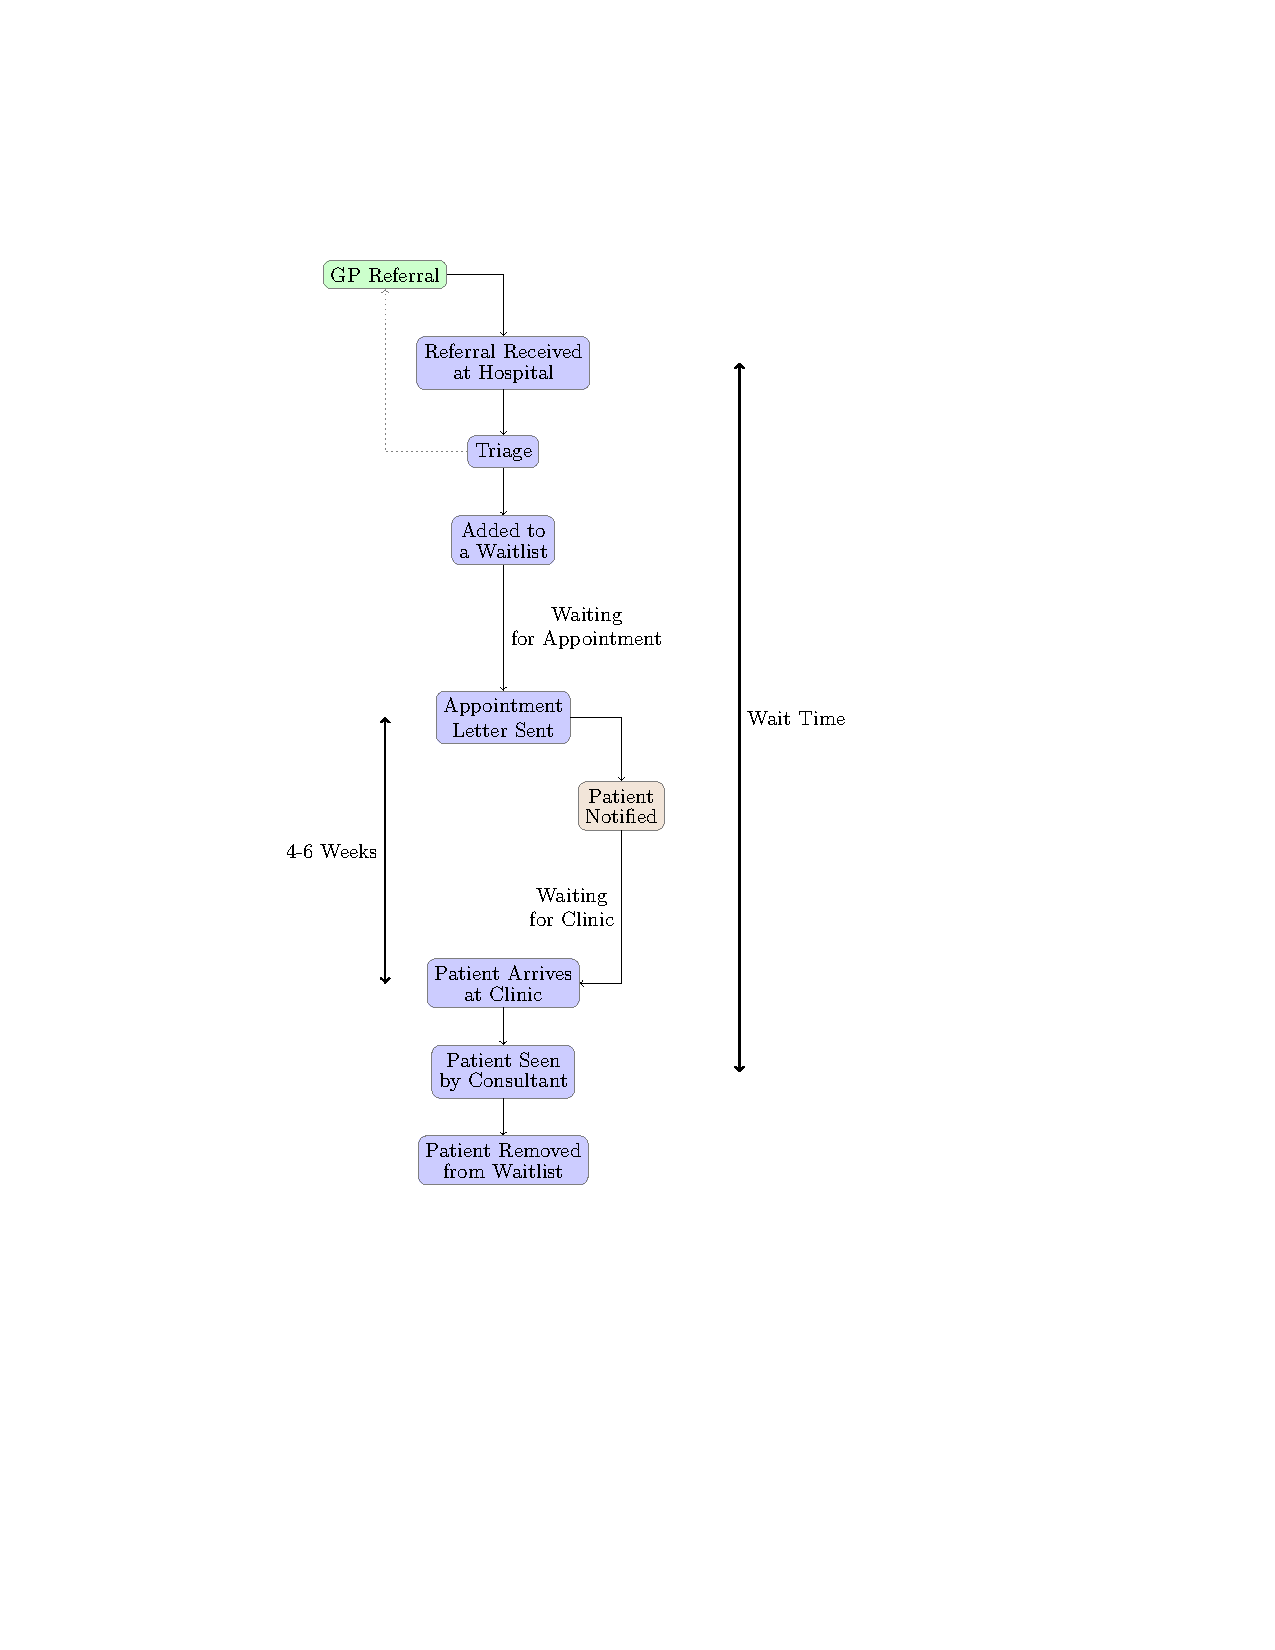
\includegraphics[width=8cm]{imagesoutpatient/process}
%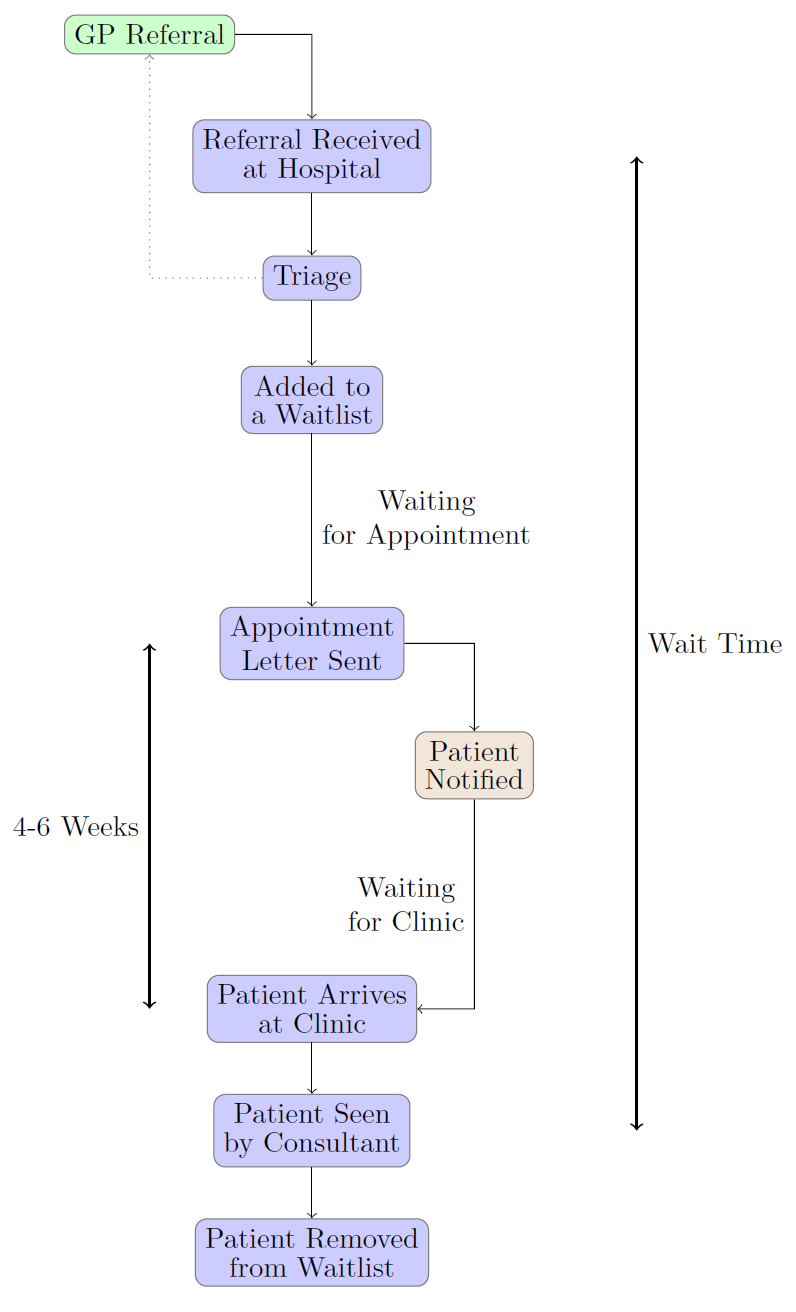
\includegraphics[width=8cm]{imagesoutpatient/processsimplified}
\scalebox{0.45}{
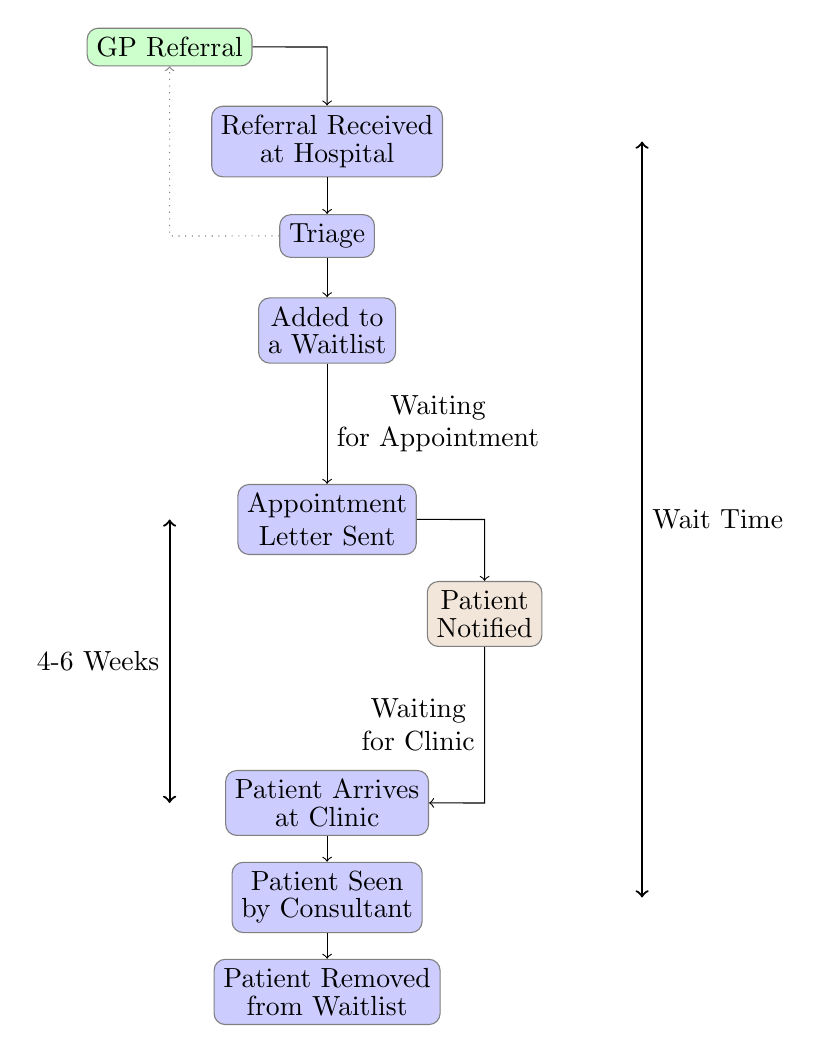
\begin{tikzpicture}[xscale=2,yscale=1.2]
  \node[draw=gray,fill=green!20,rounded corners] (referral) at (1,10) {GP Referral};
  \node[draw=gray,fill=blue!20,rounded corners] (receipt) at (2,9) {\shortstack{Referral Received\\at Hospital}};
  \node[draw=gray,fill=blue!20,rounded corners] (triage) at (2,8) {Triage};
  \node[draw=gray,fill=blue!20,rounded corners] (waitlist) at (2,7) {\shortstack{Added to\\a Waitlist}};
  \node[draw=gray,fill=blue!20,rounded corners] (appointment) at (2,5) {\shortstack{Appointment\\Letter Sent}};
  \node[draw=gray,fill=brown!20,rounded corners] (notified) at (3,4) {\shortstack{Patient\\Notified}};
  \node[draw=gray,fill=blue!20,rounded corners] (arrival) at (2,2) {\shortstack{Patient Arrives\\at Clinic}};
  \node[draw=gray,fill=blue!20,rounded corners] (seen) at (2,1) {\shortstack{Patient Seen\\by Consultant}};
  \node[draw=gray,fill=blue!20,rounded corners] (removed) at (2,0) {\shortstack{Patient Removed\\from Waitlist}};
  \draw[->] (referral) -- (2,10) -- (receipt);
  \draw[->] (receipt) -- (triage);
  \draw[->] (triage) -- (waitlist);
  \draw[->,dotted,gray] (triage) -- (1,8) -- (referral);
  \draw[->] (waitlist) -- node[right] {\shortstack{Waiting\\for Appointment}} (appointment);
  \draw[->] (appointment) -- (3,5) -- (notified);
  \draw[->] (notified) -- node[left] {\shortstack{Waiting\\for Clinic}} (3,2) -- (arrival);
  \draw[->] (arrival) -- (seen);
  \draw[->] (seen) -- (removed);
  \draw[<->,thick] (4,9) -- node[right] {Wait Time} (4,1);
  \draw[<->,thick] (1,5) -- node[left] {4-6 Weeks} (1,2);
\end{tikzpicture}
}

\end{frame}

% \begin{frame}
% \frametitle{National Waitlist Management Protocol (2017)}
% \begin{tabular}{@{}c@{ }c@{ }c@{ }c@{ }c@{}}
% 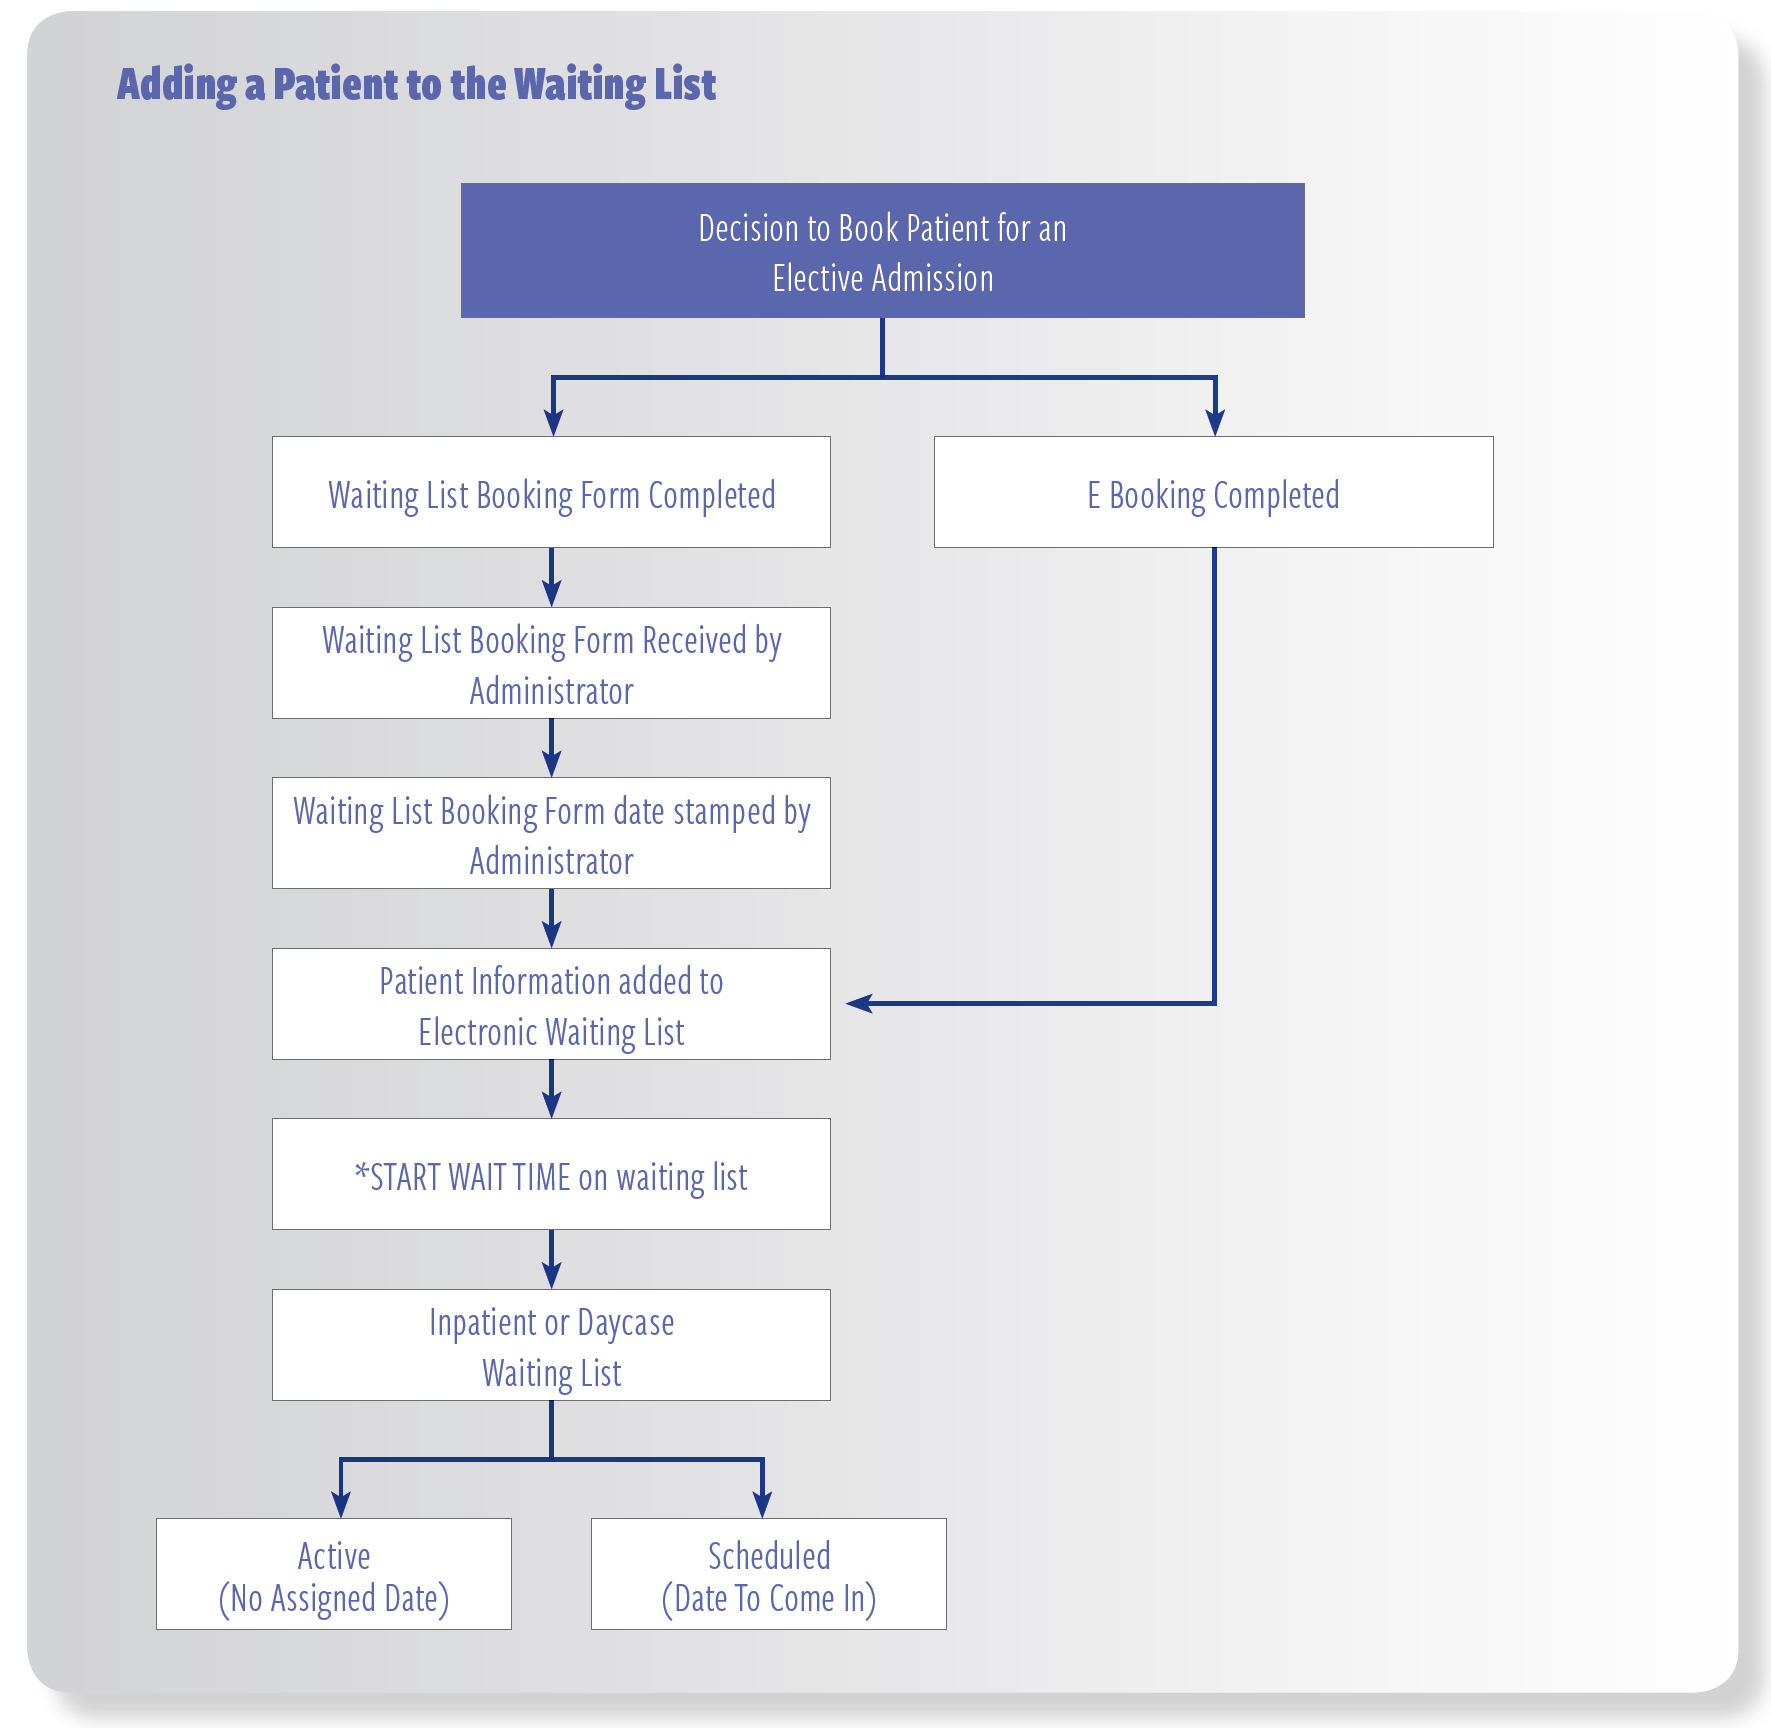
\includegraphics[width=2cm]{imagesoutpatient/addingtowaitlist} &
% 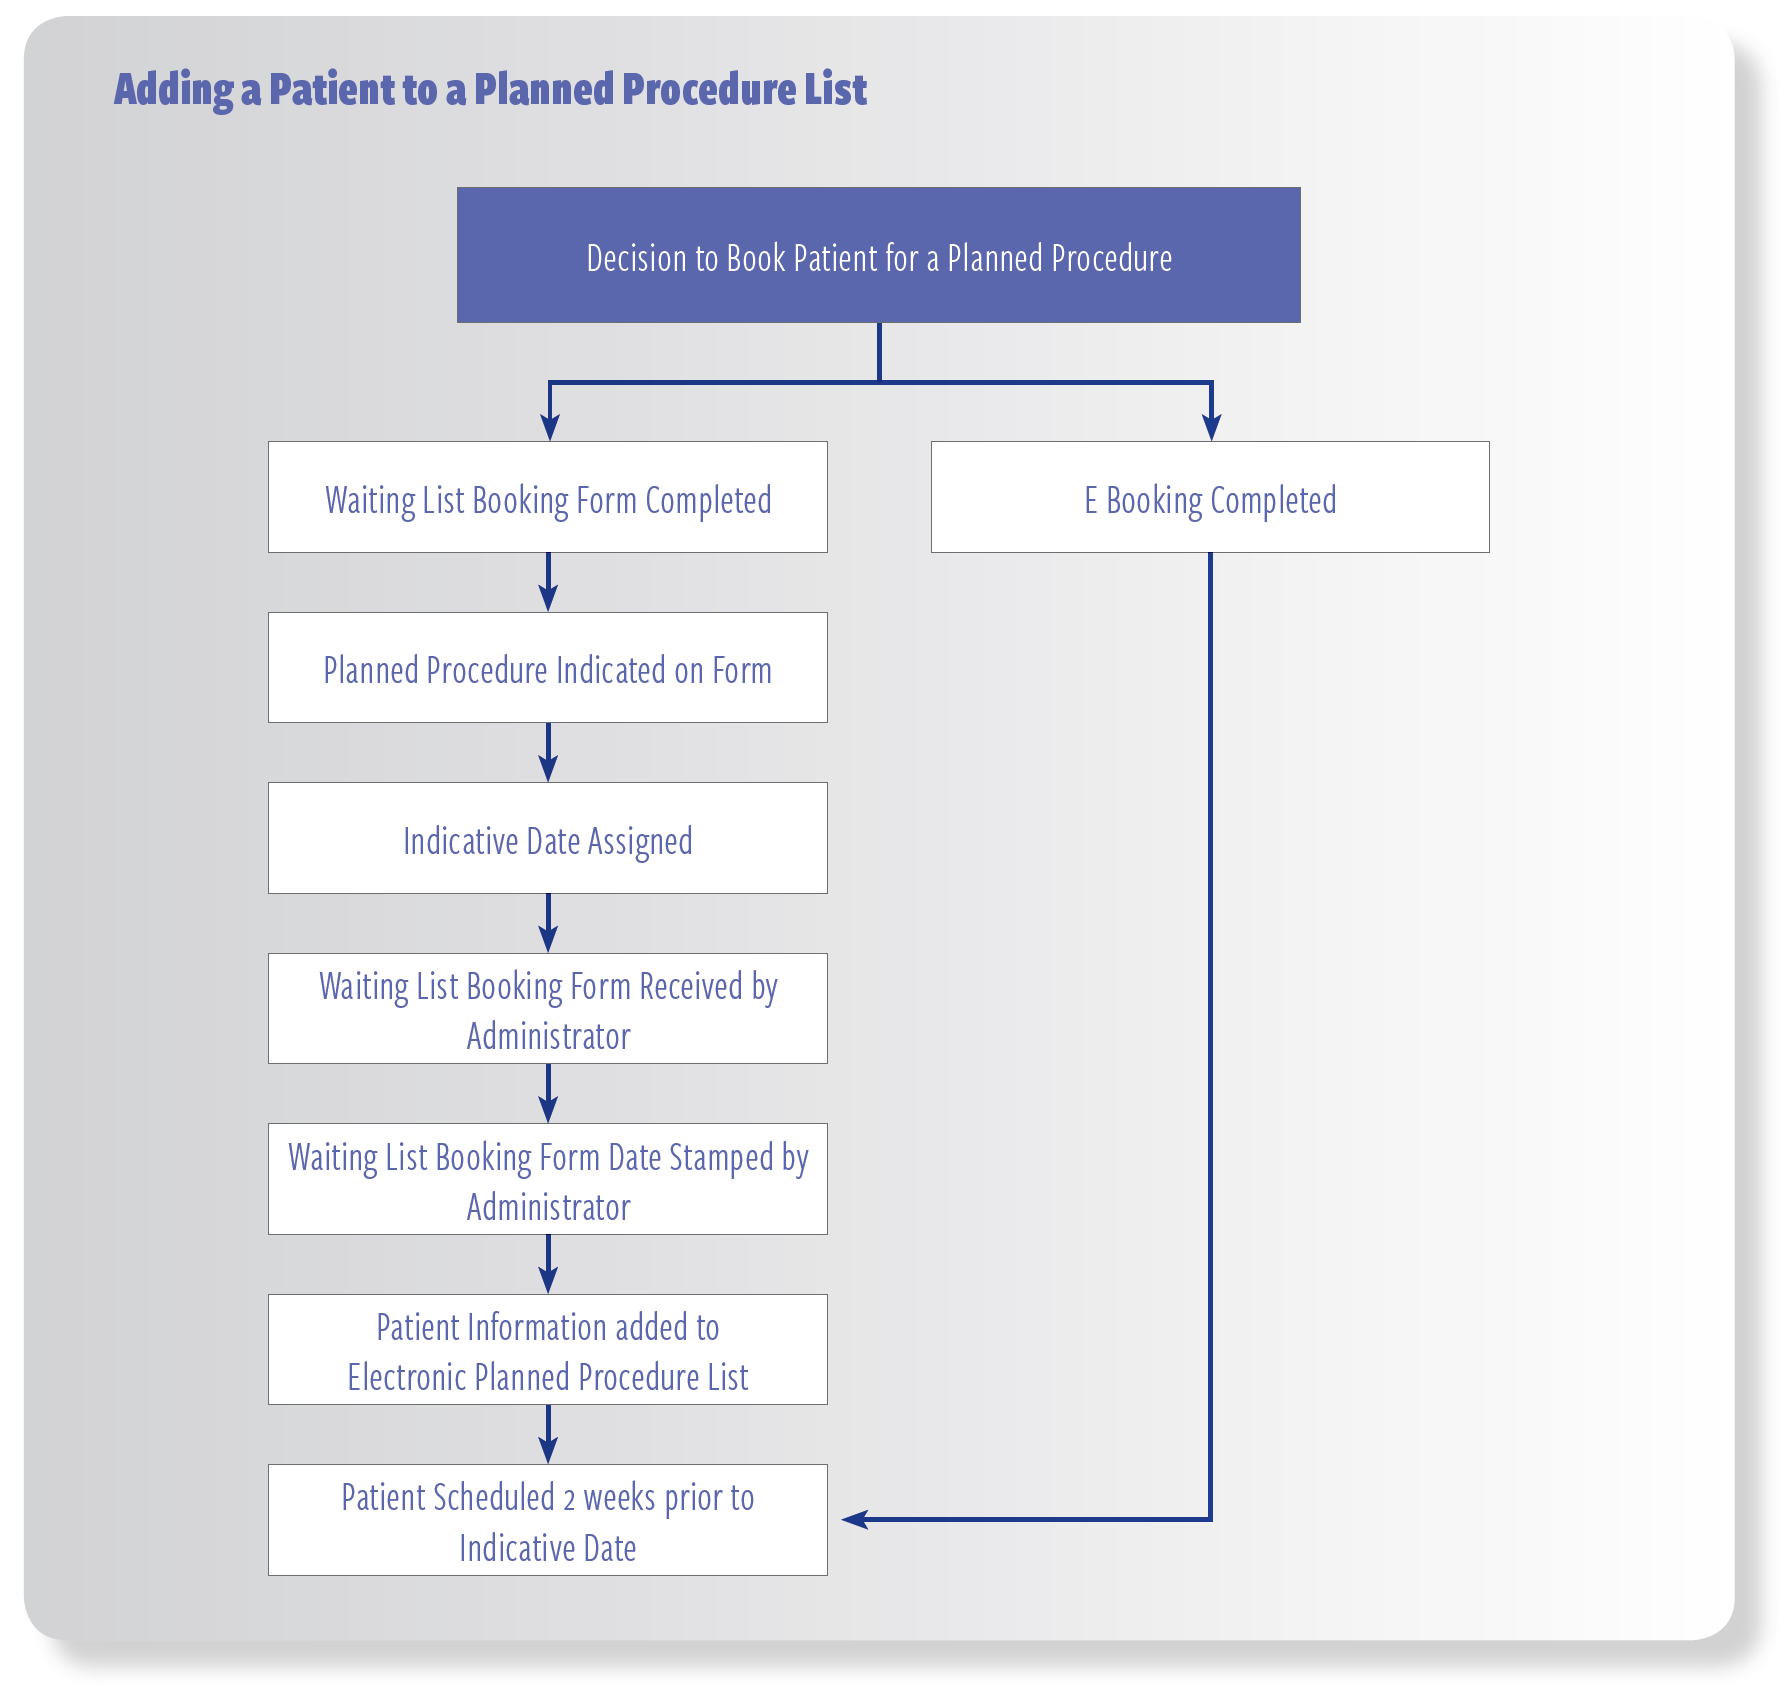
\includegraphics[width=2cm]{imagesoutpatient/addingtoplannedprocedure} &
% 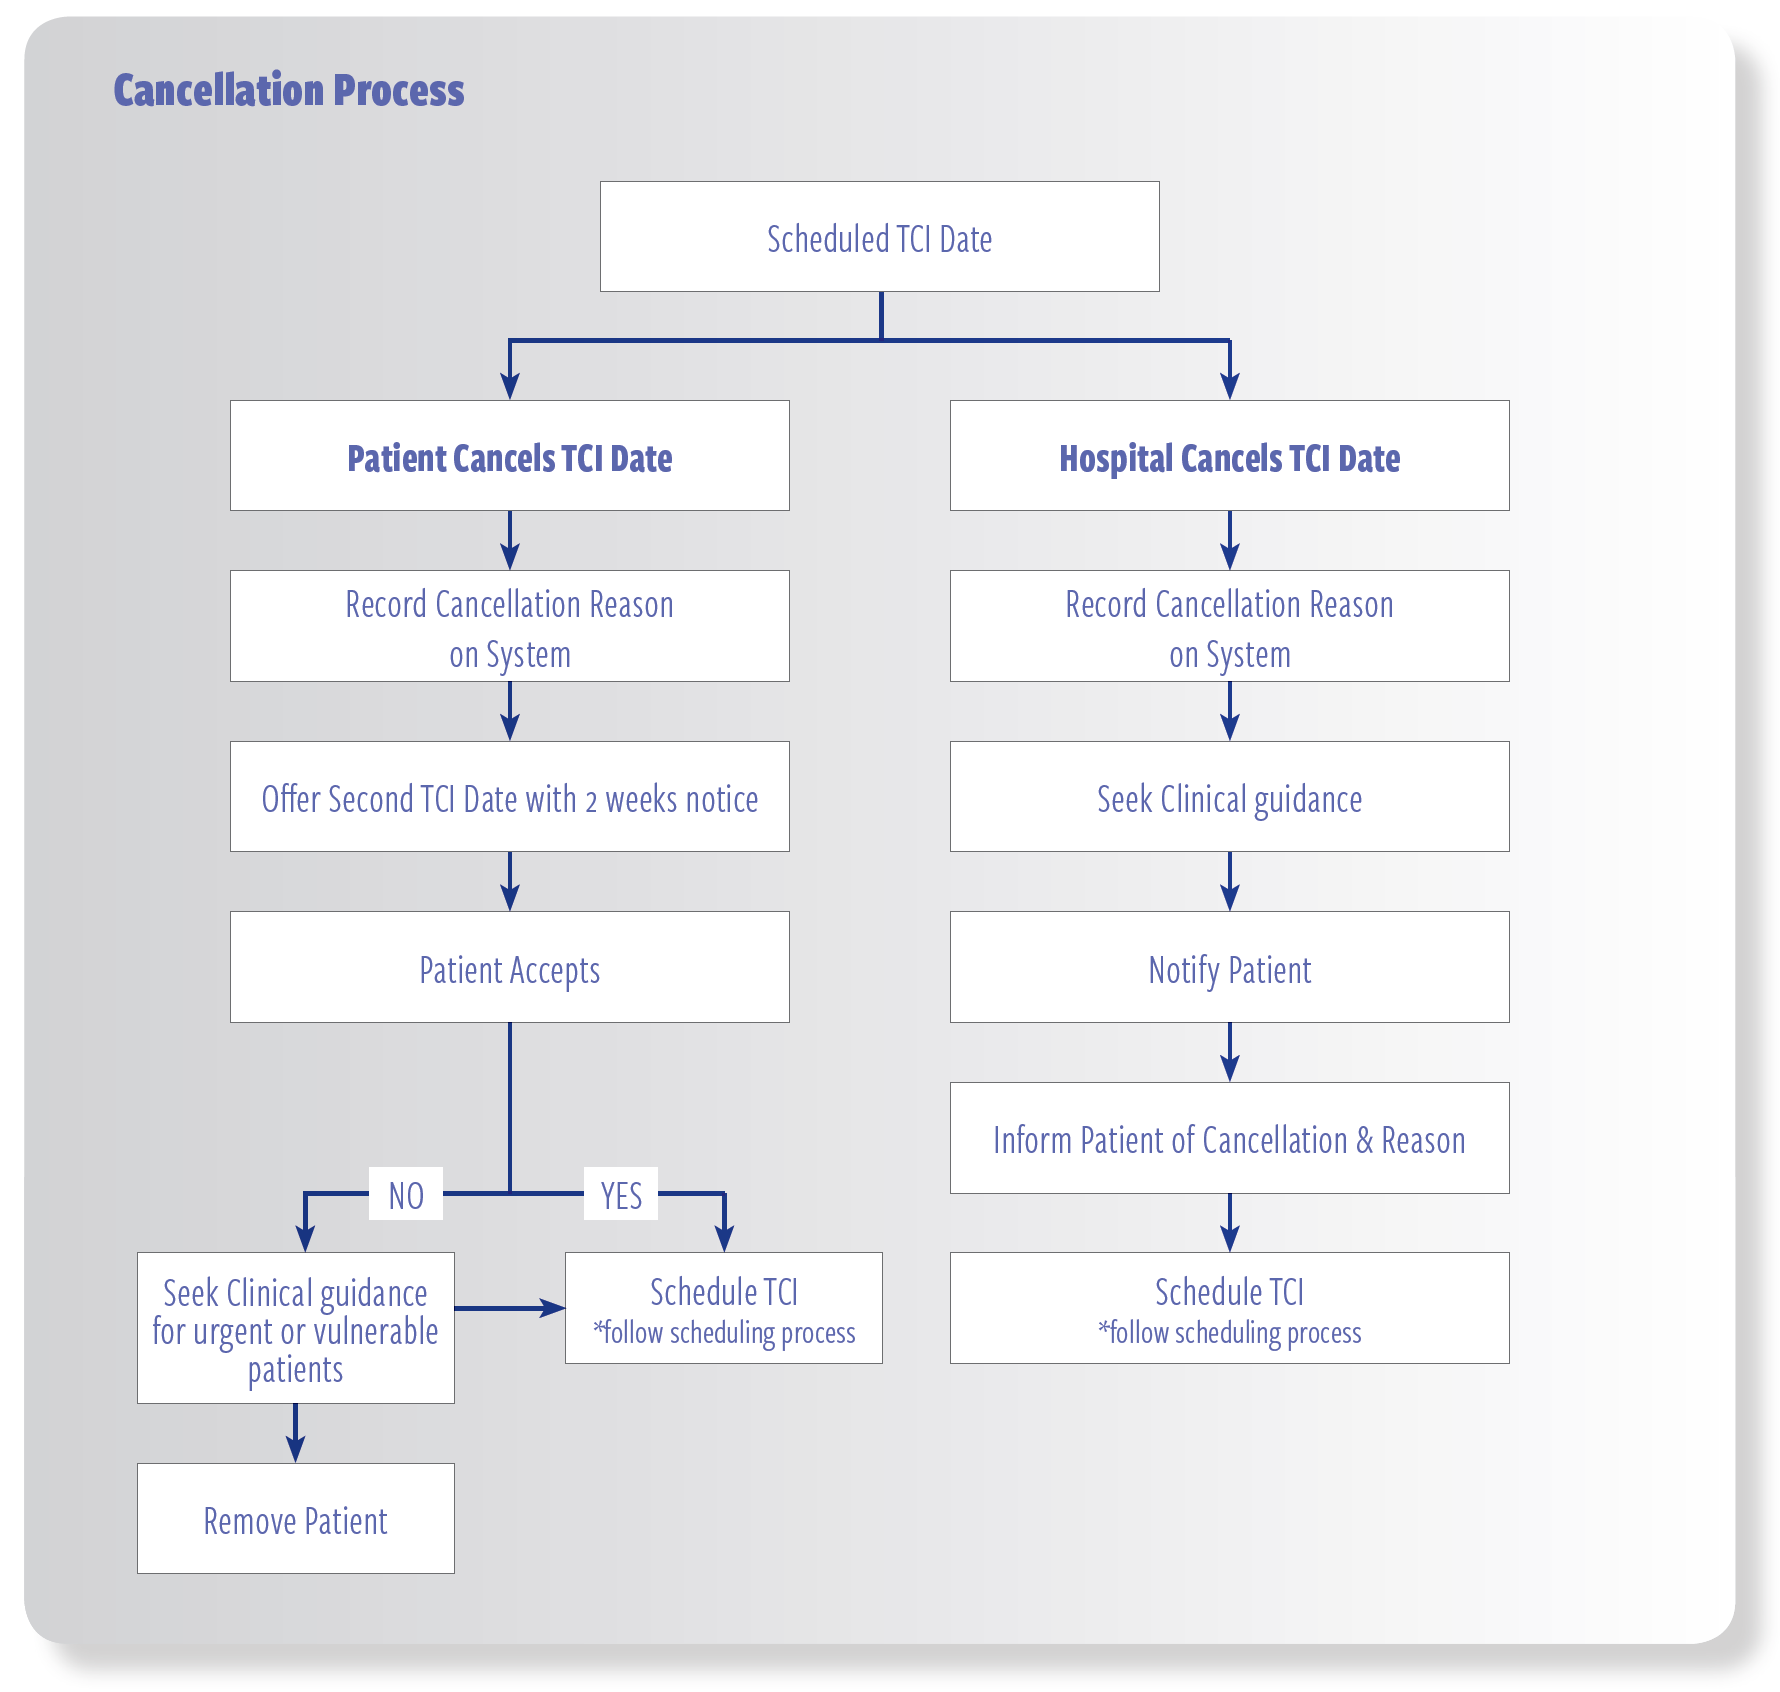
\includegraphics[width=2cm]{imagesoutpatient/cancellationprocess} &
% 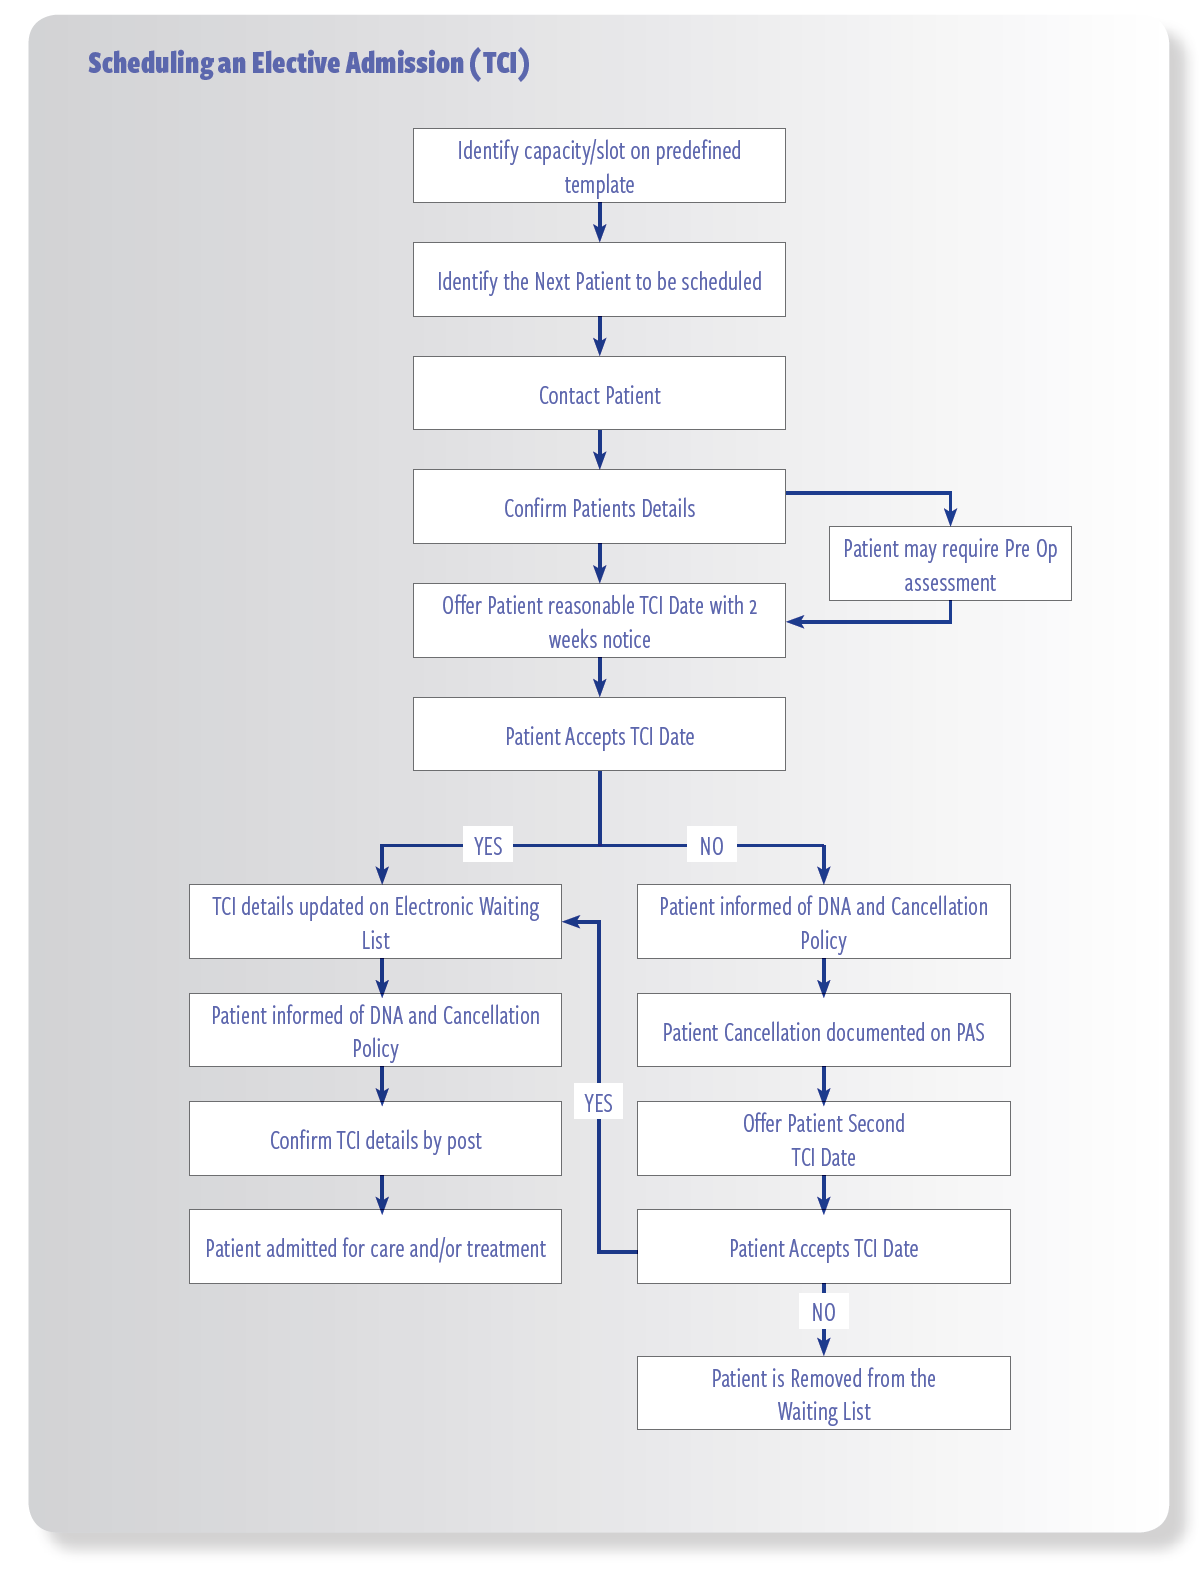
\includegraphics[width=2cm]{imagesoutpatient/schedulingadmission} &
% 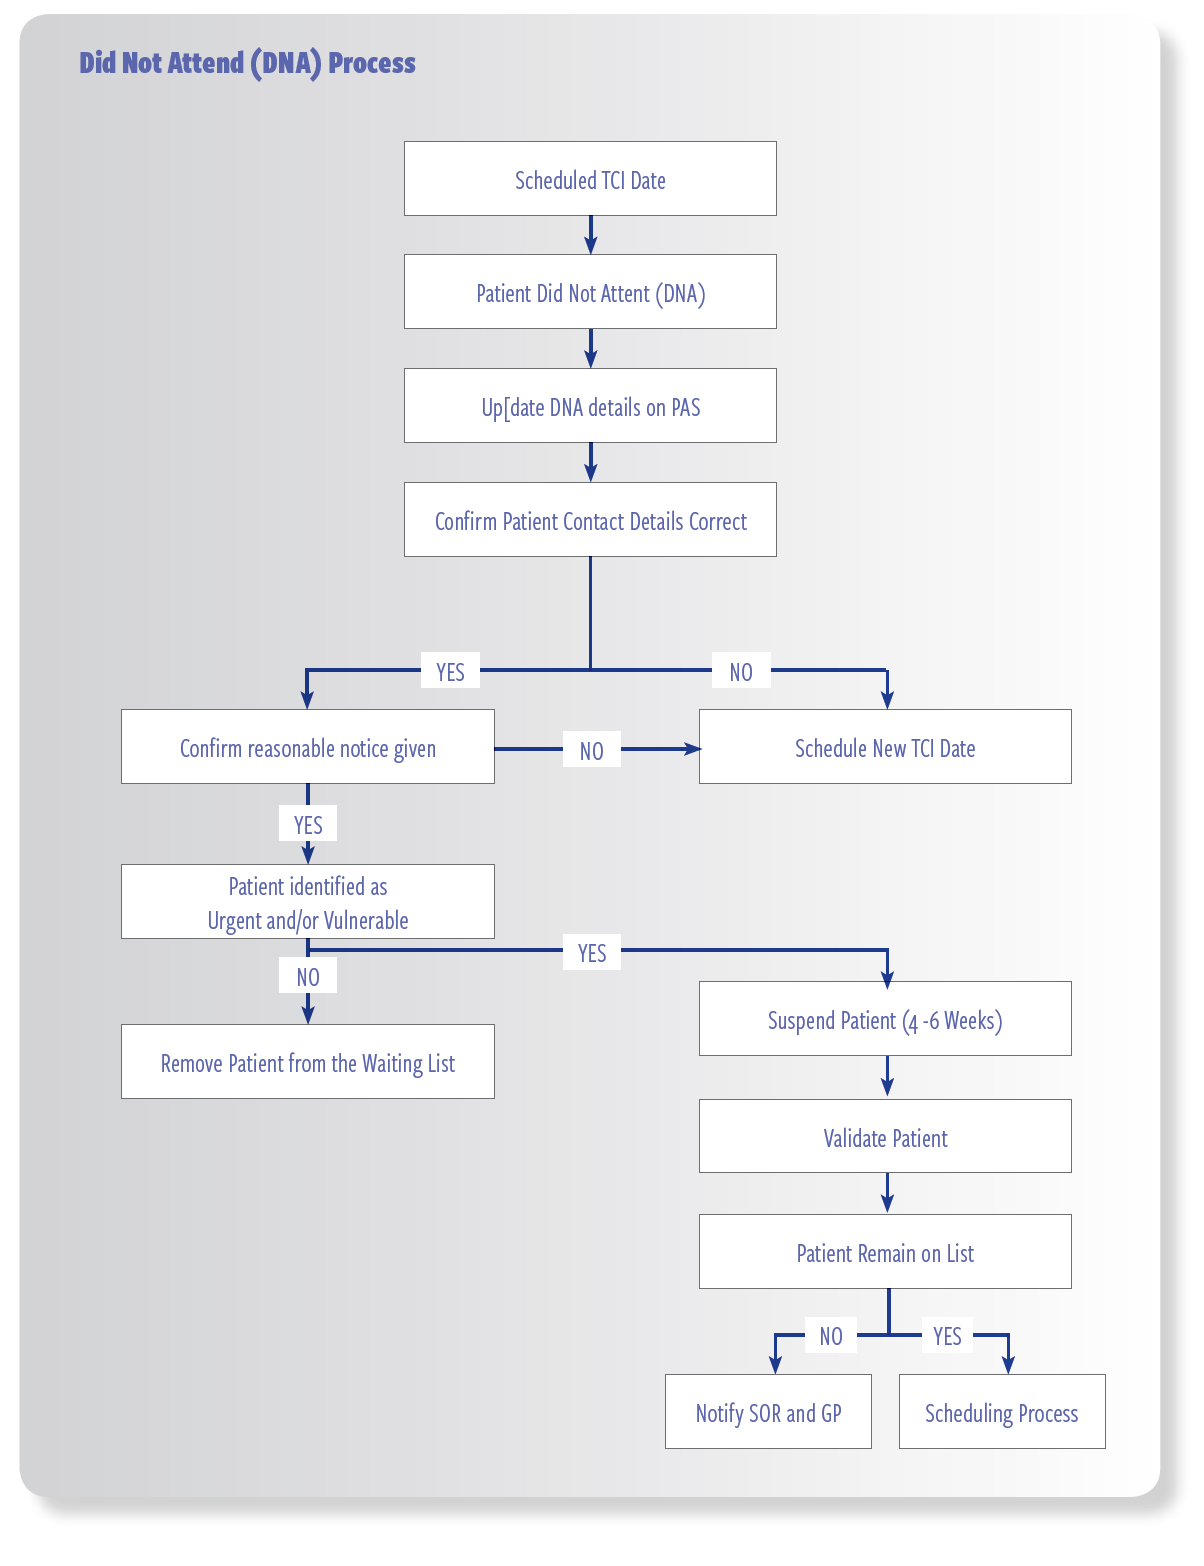
\includegraphics[width=2cm]{imagesoutpatient/dnaprocess} \\
% 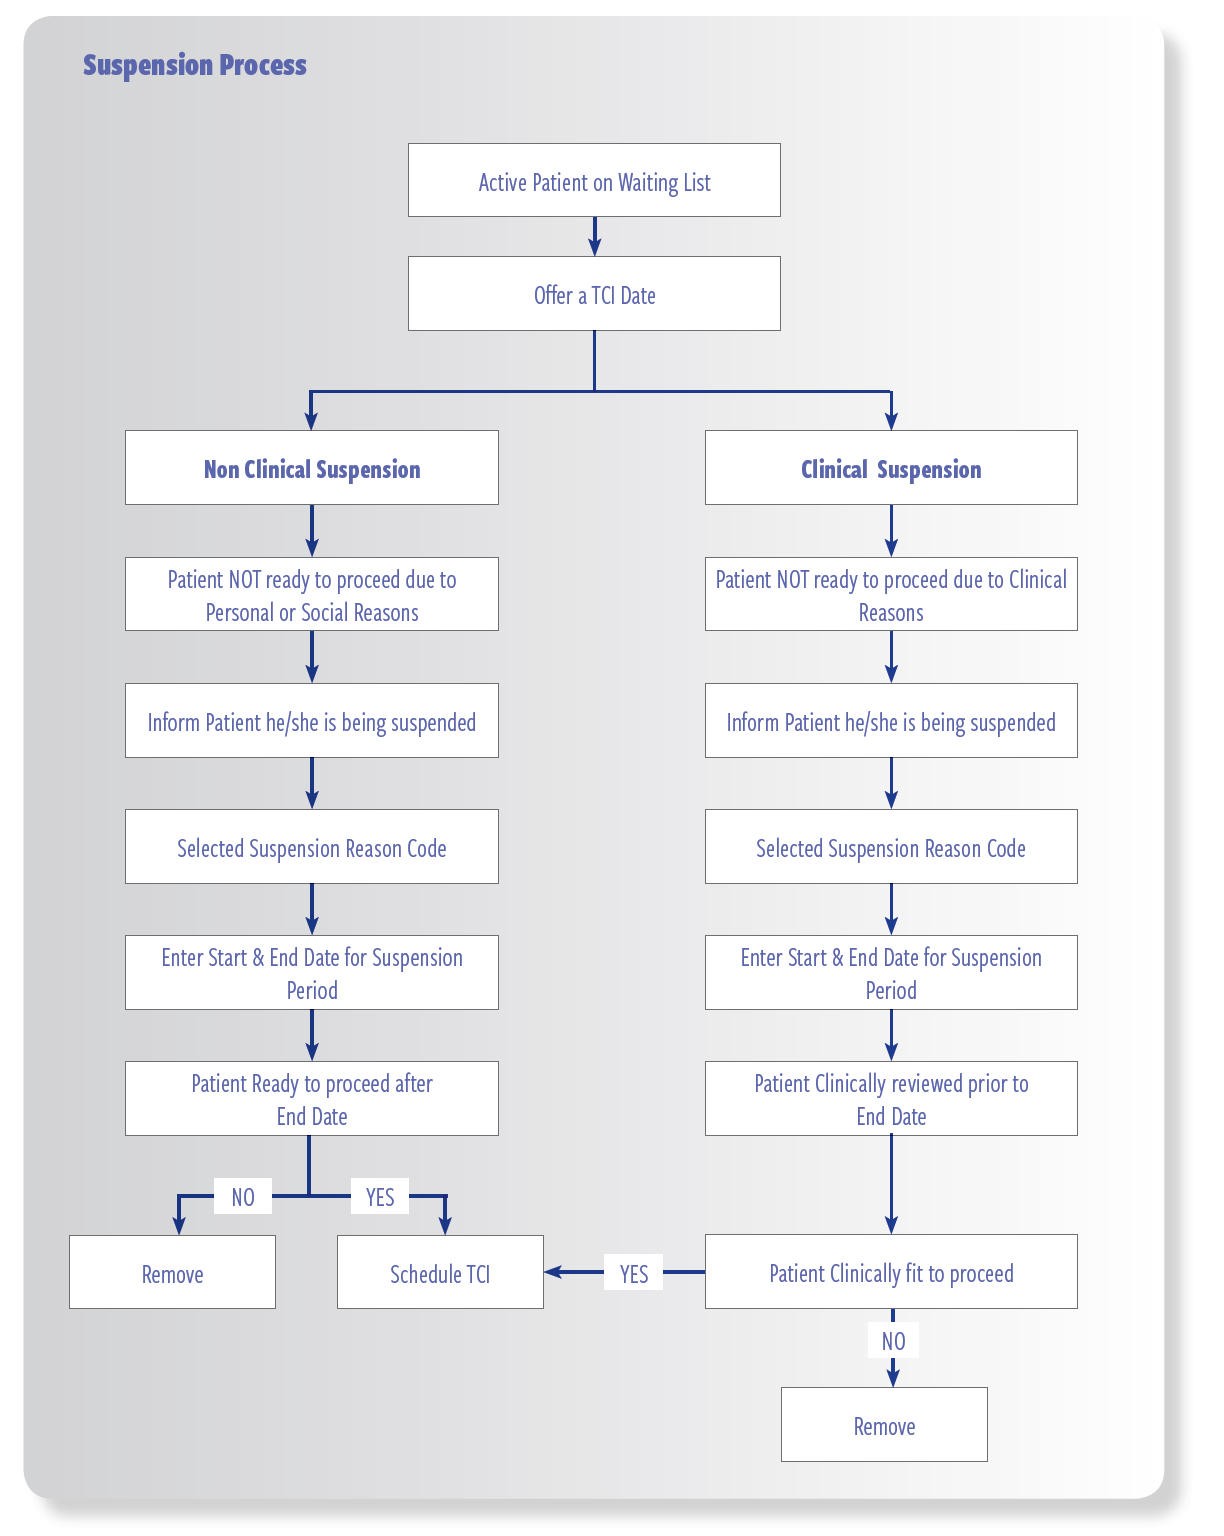
\includegraphics[width=2cm]{imagesoutpatient/suspensionprocess} &
% 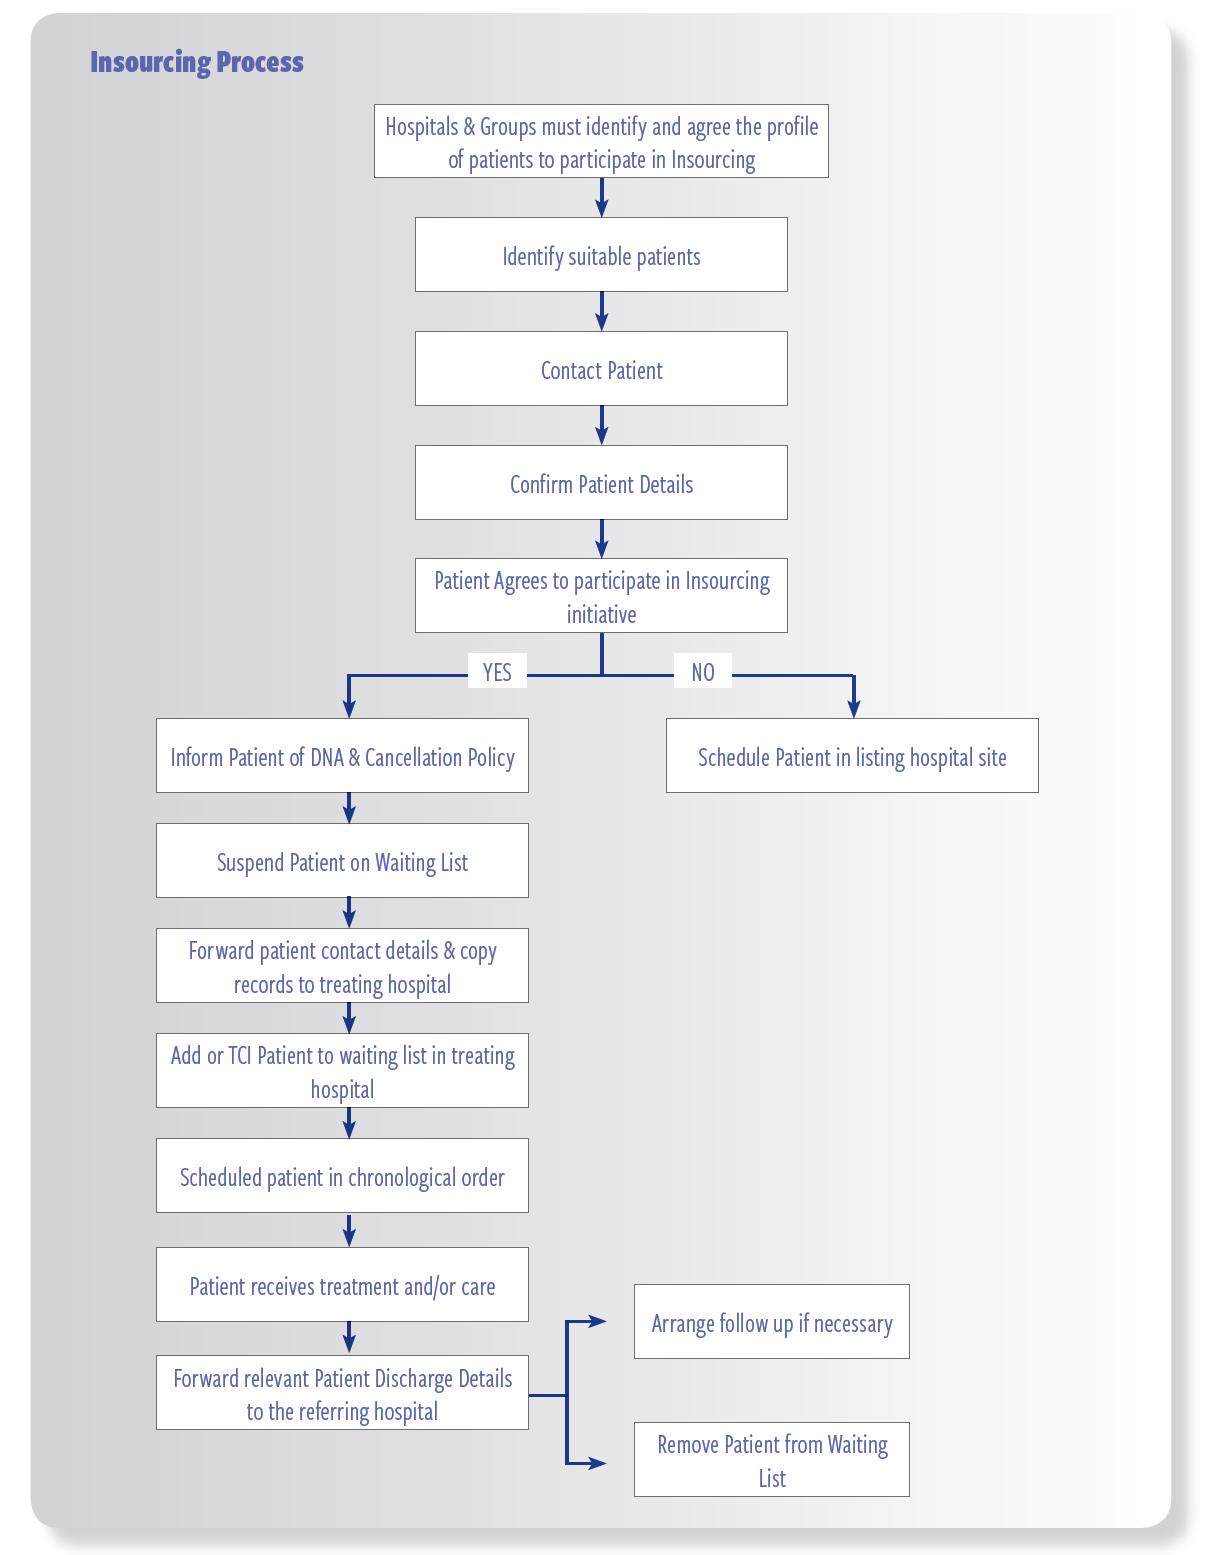
\includegraphics[width=2cm]{imagesoutpatient/insourcingprocess} &
% 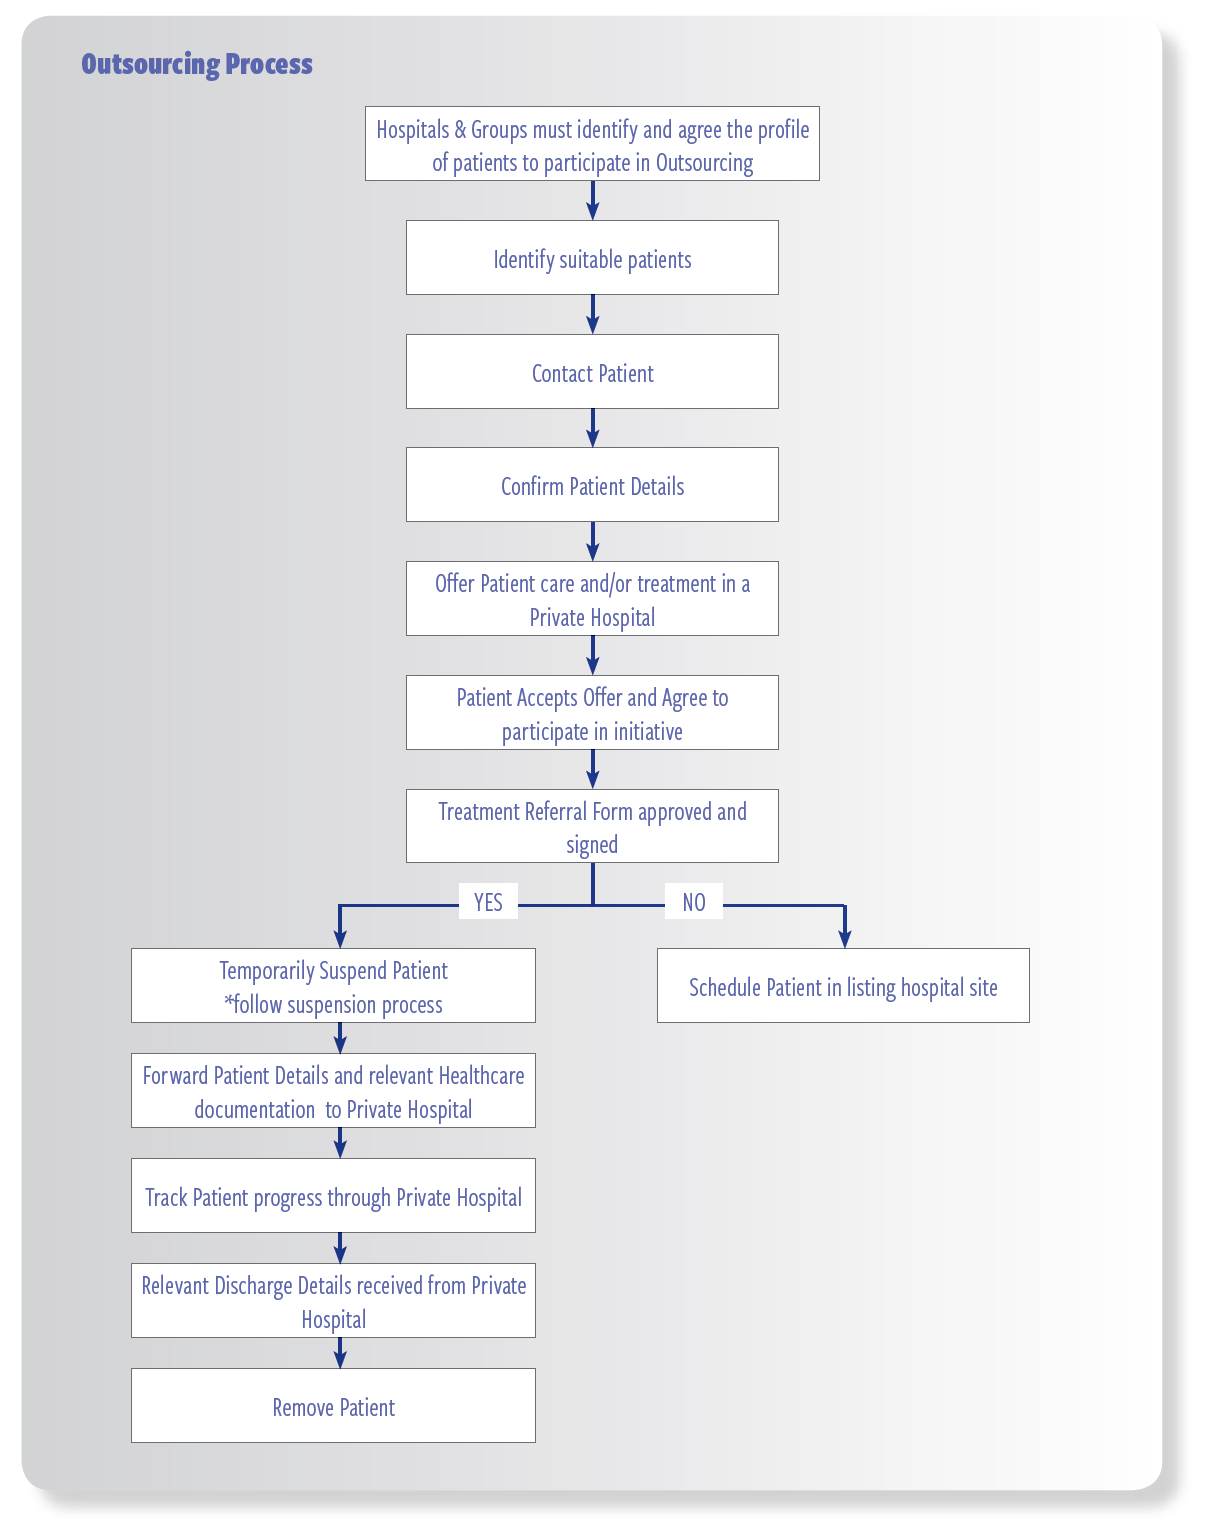
\includegraphics[width=2cm]{imagesoutpatient/outsourcingprocess} &
% 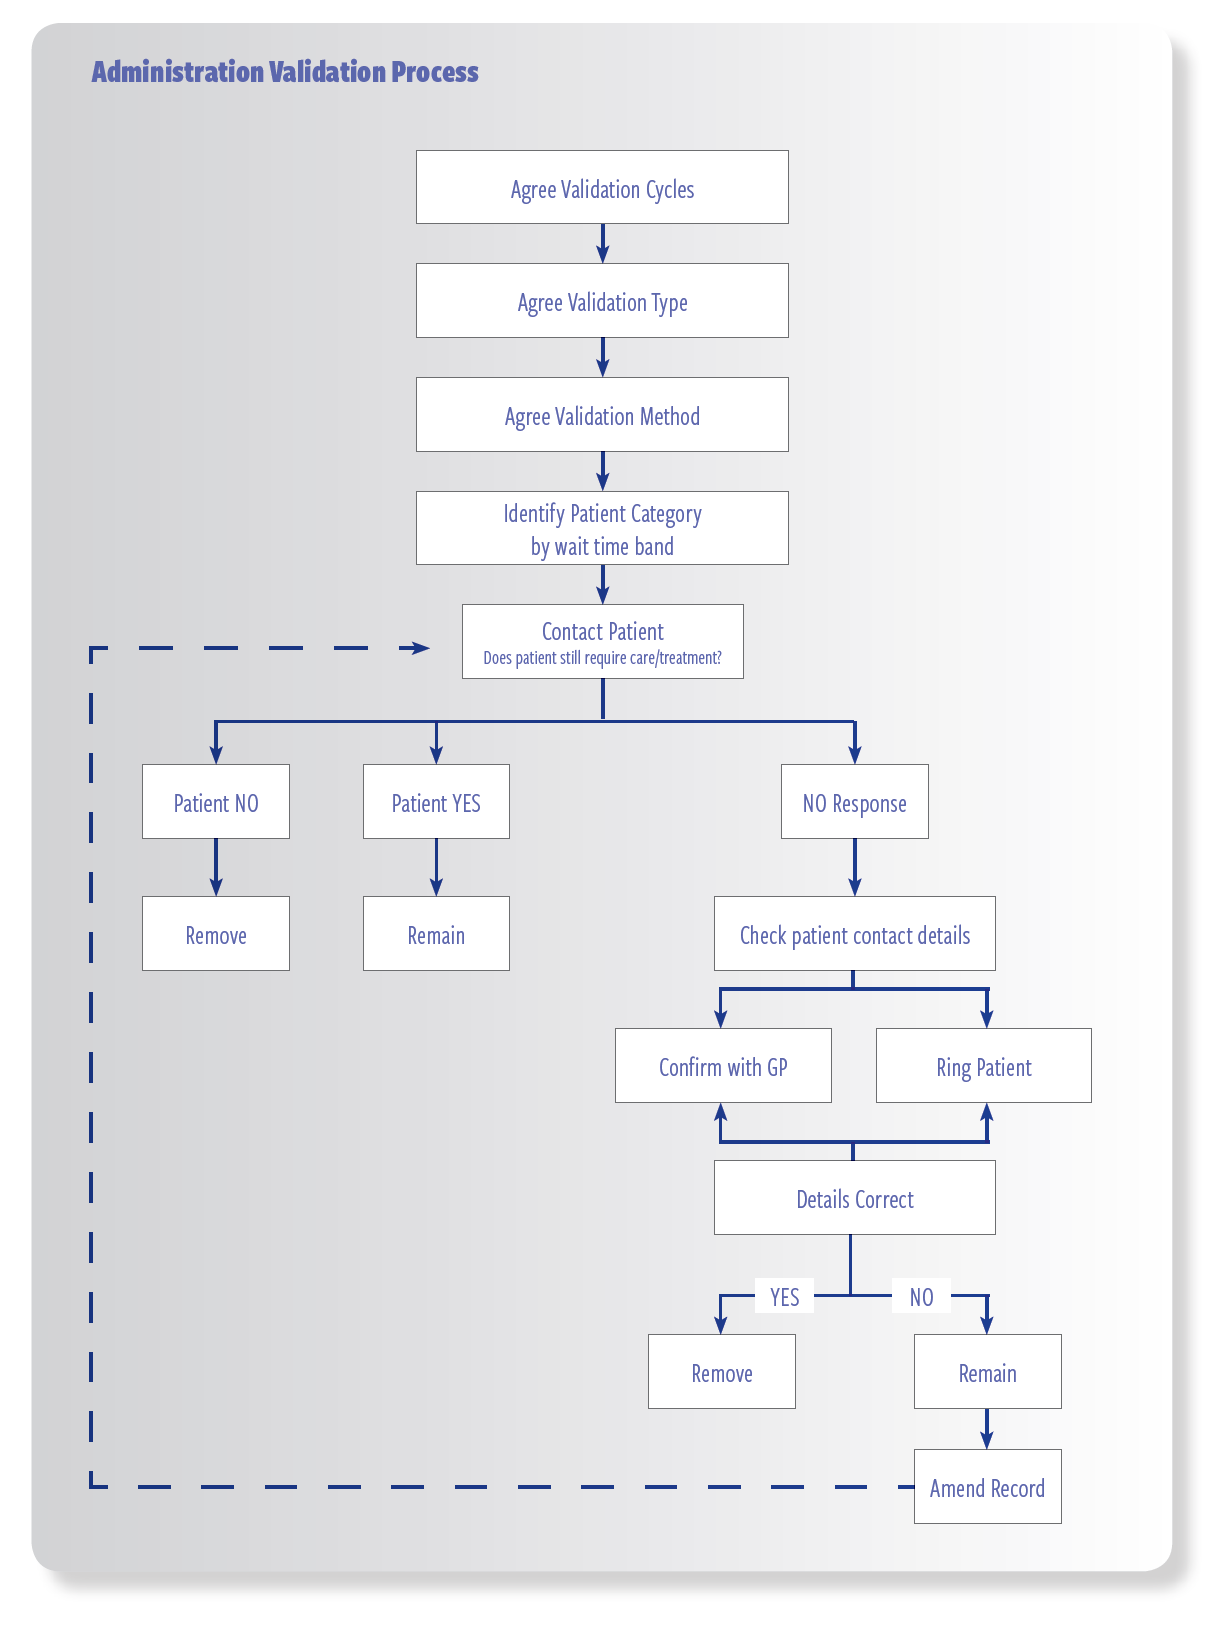
\includegraphics[width=2cm]{imagesoutpatient/validationprocess} &
% 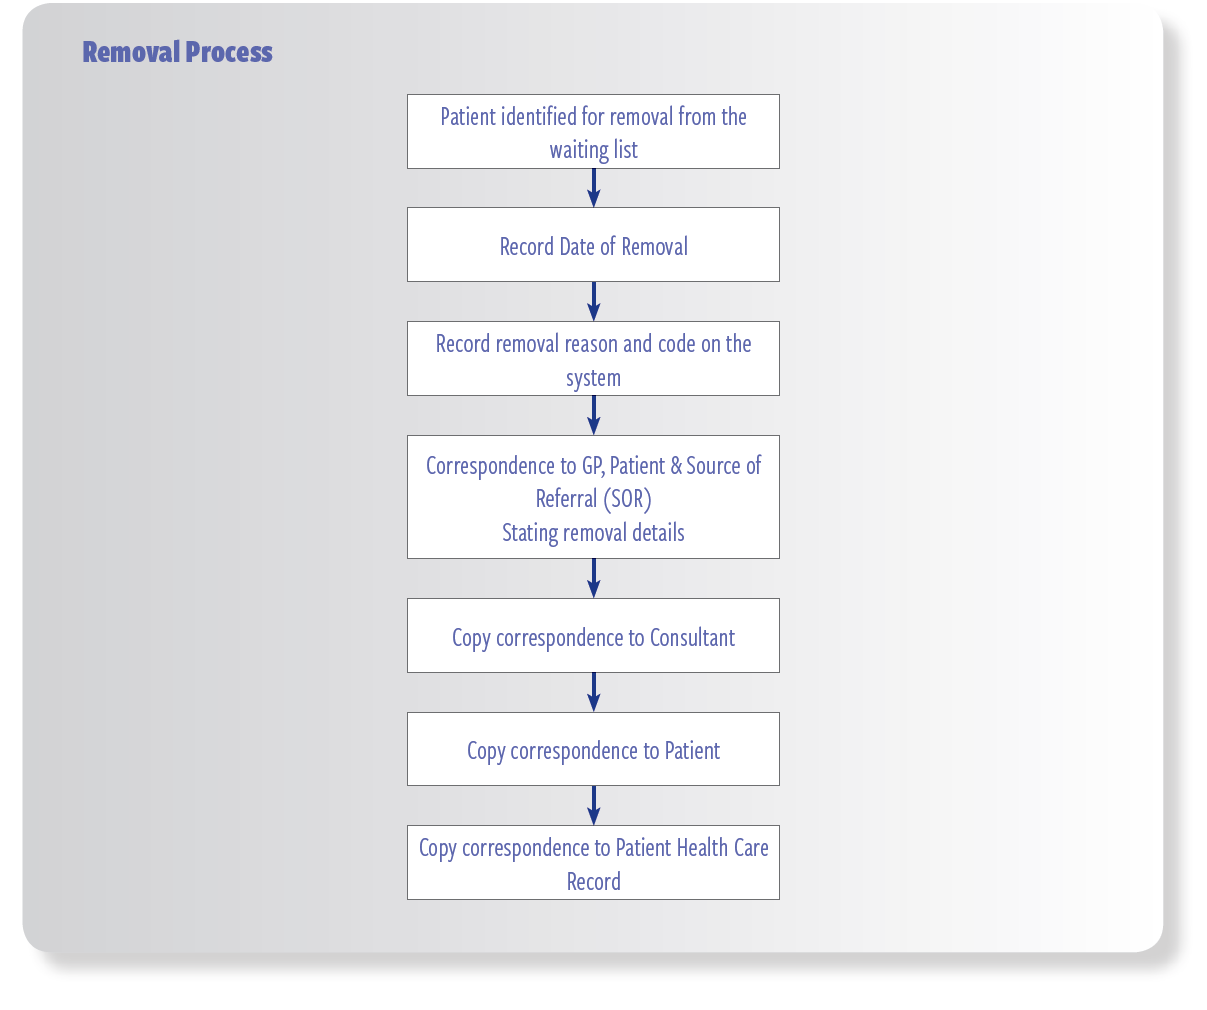
\includegraphics[width=2cm]{imagesoutpatient/removalprocess} 
% \end{tabular}

% \vspace{0.5cm}
% {\scriptsize Inpatient/DayCase Process Shown, Outpatient Document Not Final}
% \end{frame}

\begin{frame}
\frametitle{The Bad News}
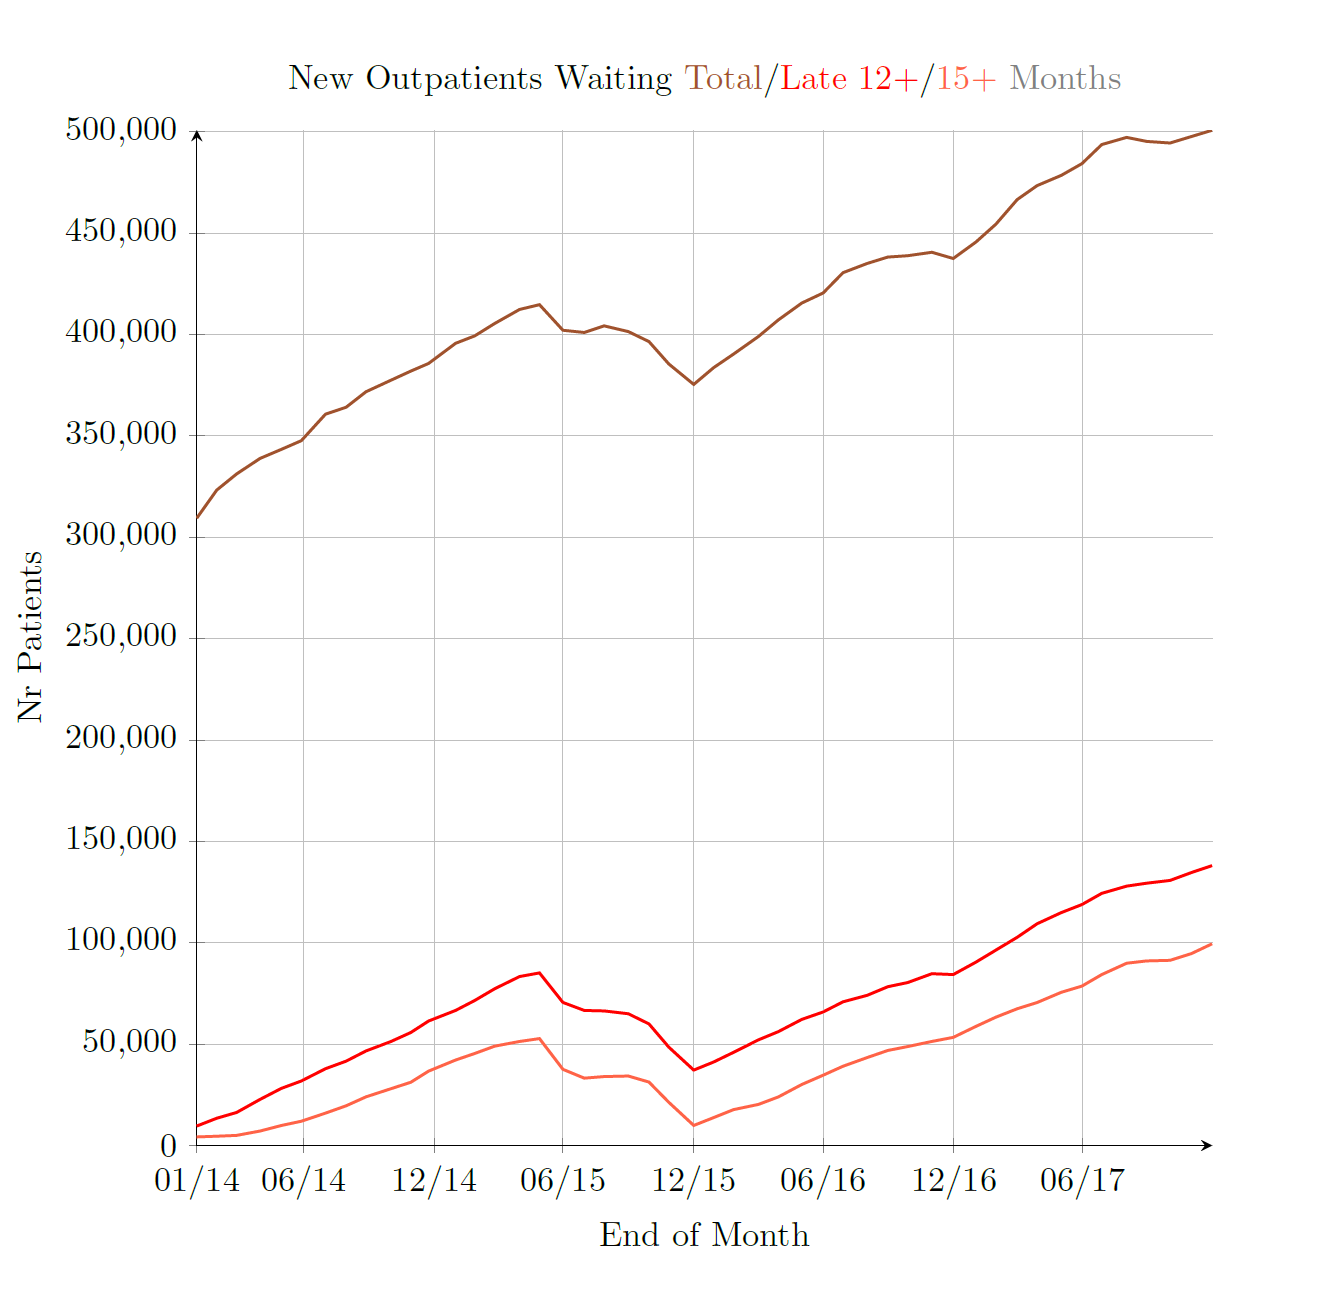
\includegraphics[width=7cm]{imagesoutpatient/newoutpatientswaitingdec2017}
{\scriptsize Data: NTPF}
\end{frame}


% \begin{frame}
% \frametitle{Patients Waiting: The Very Bad News}
% %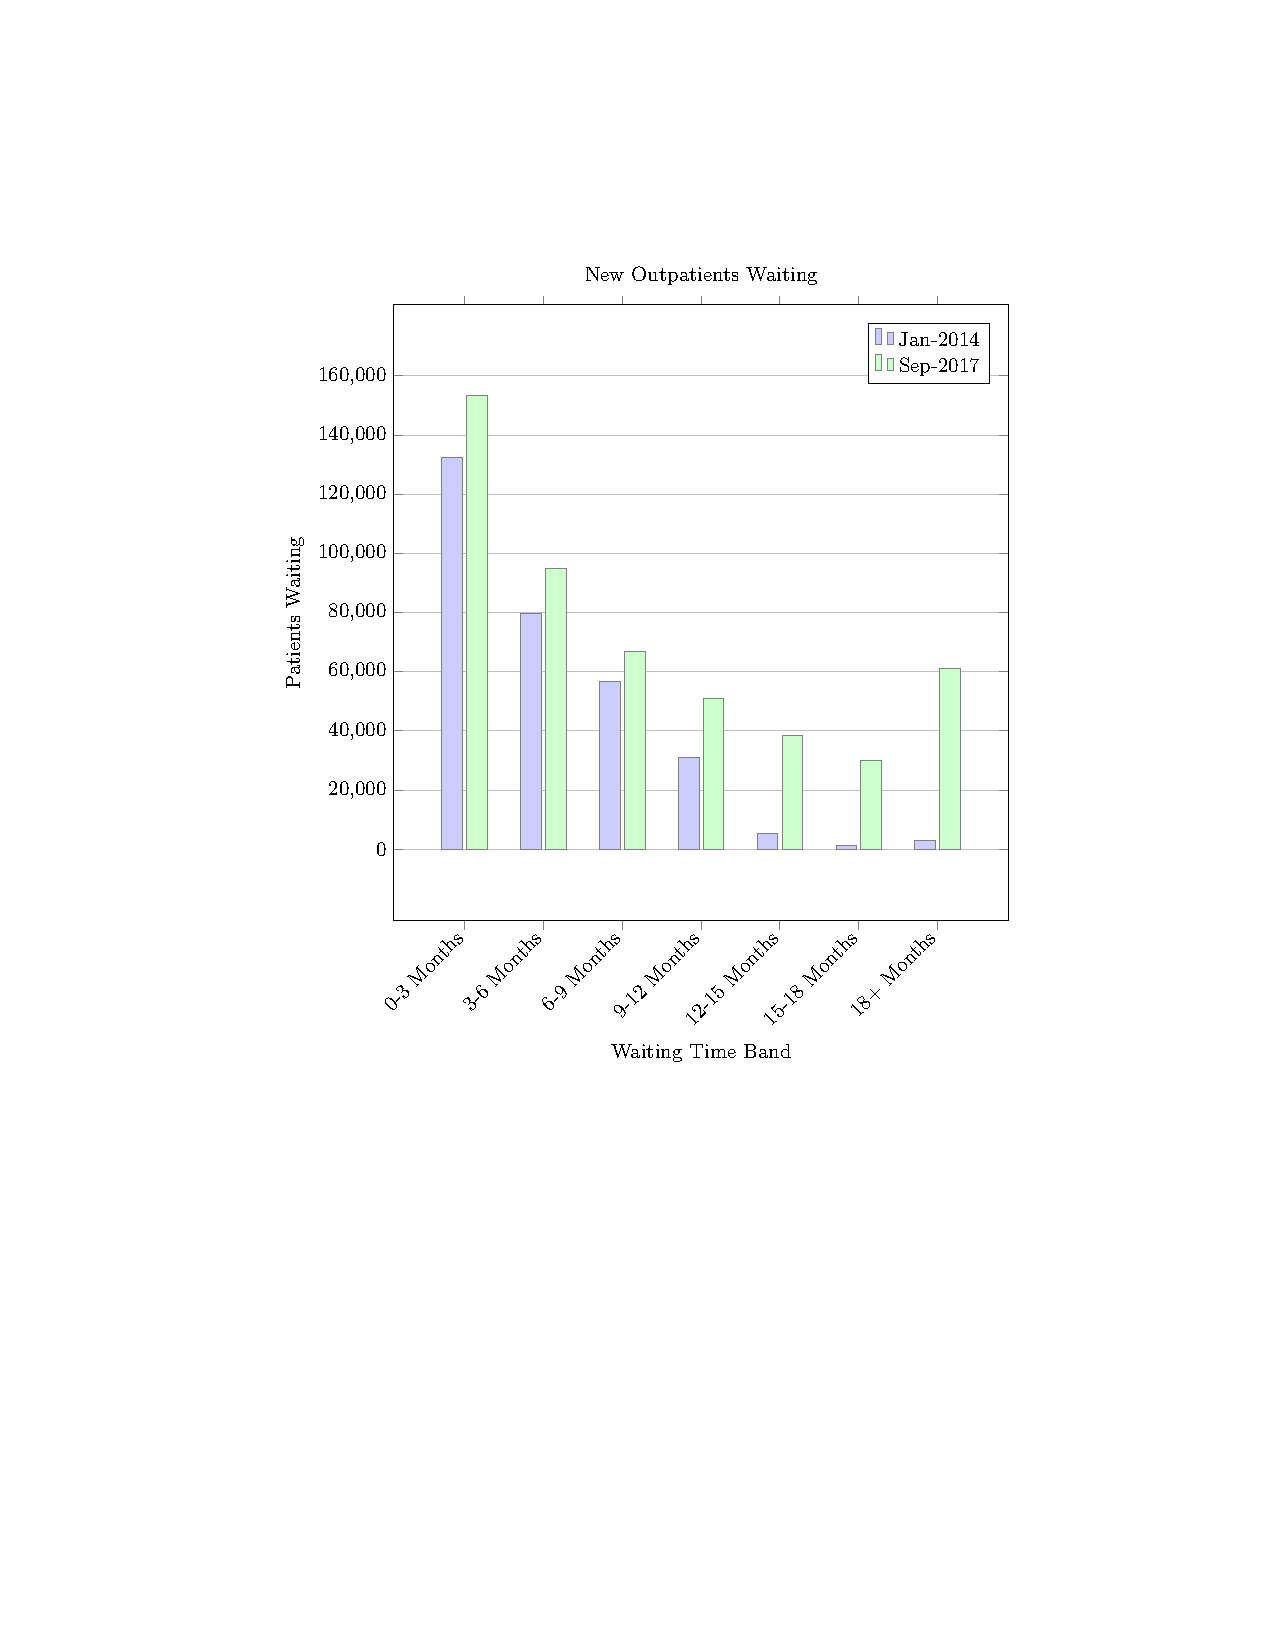
\includegraphics[width=9cm]{imagesoutpatient/waitingband2}
% 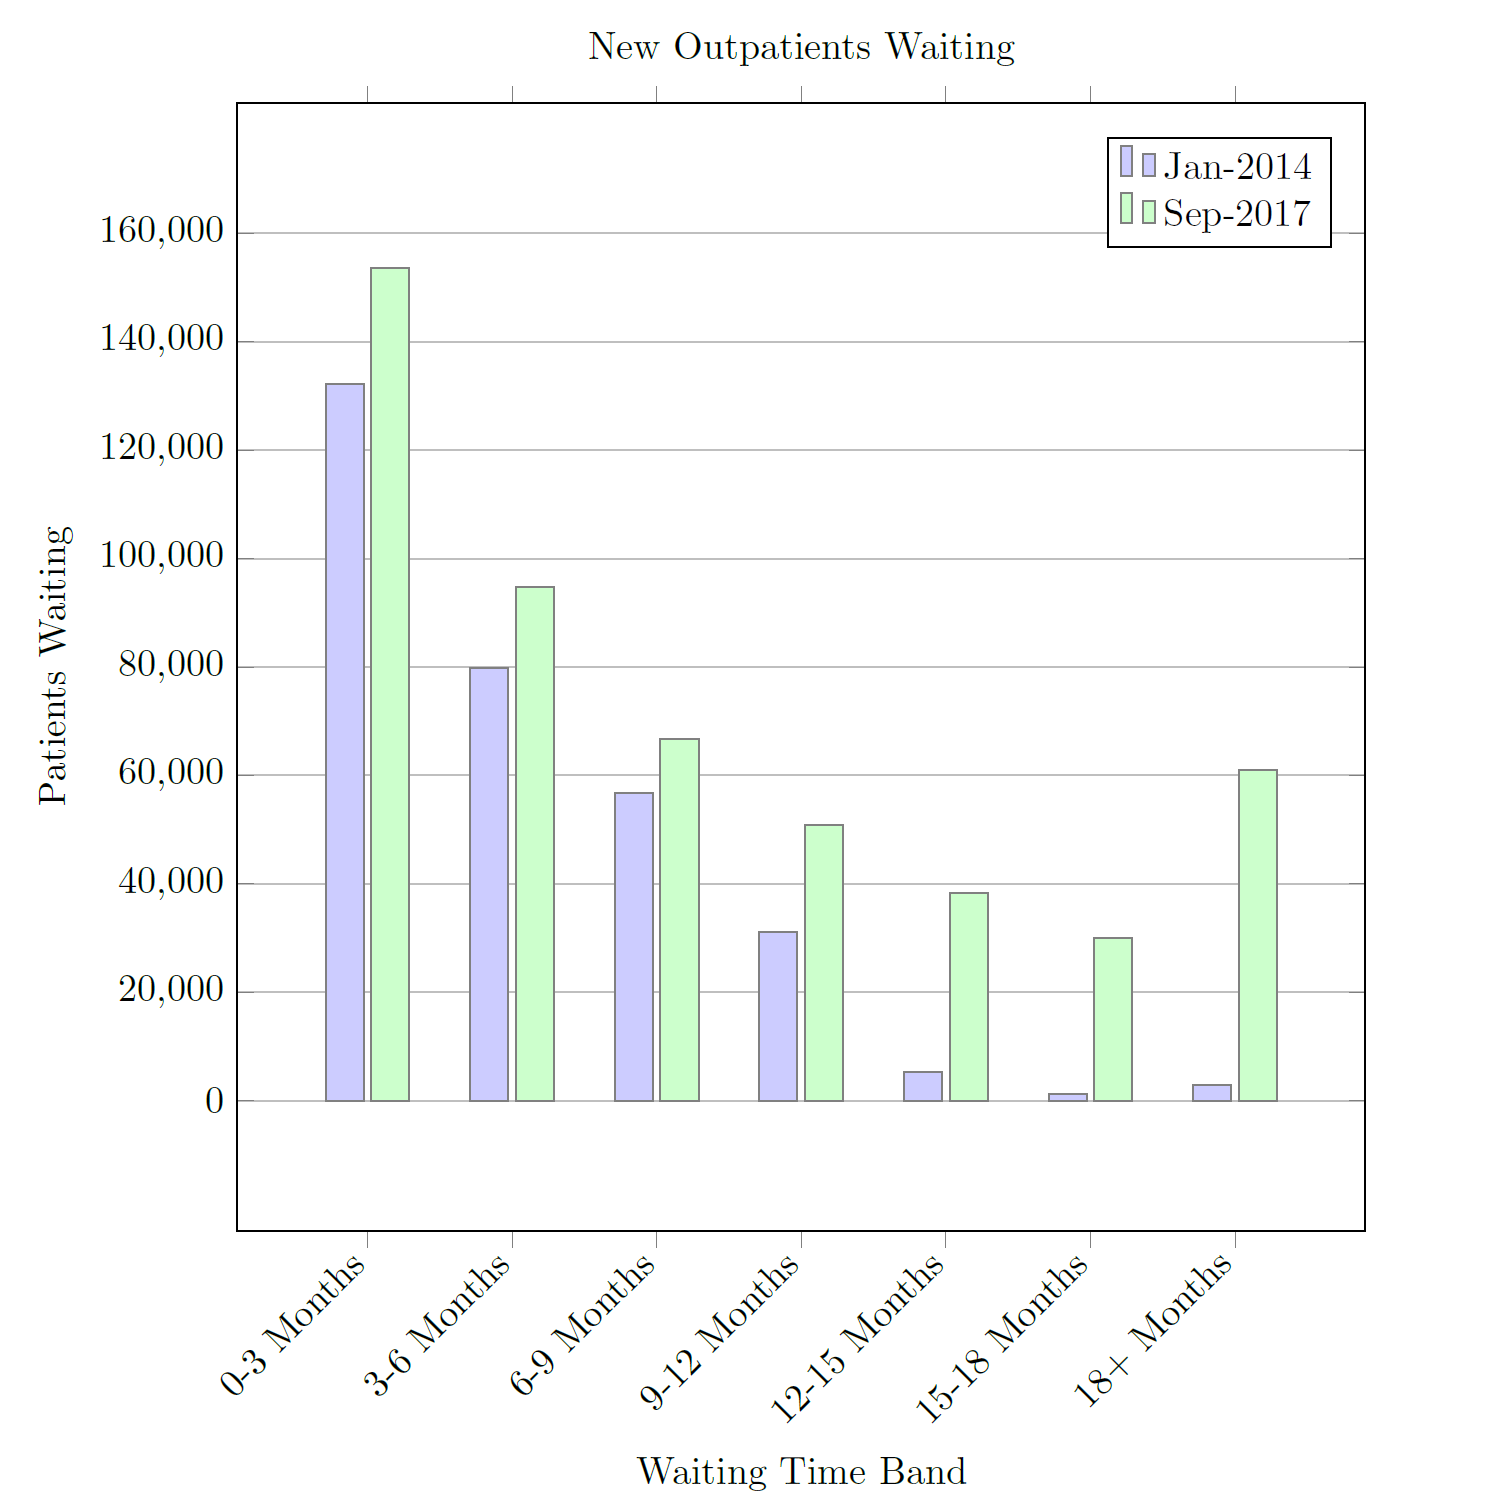
\includegraphics[width=7cm]{imagesoutpatient/newoutpatientswaitingbands}
% {\scriptsize Data: NTPF}
% \end{frame}

%% \begin{frame}
%% \frametitle{Patients Waiting: Age Groups}
%% \includegraphics[width=9cm]{imagesoutpatient/waitingagegroup}
%% \end{frame}

\begin{frame}
\frametitle{KPI: Waiting Time Percentage}
\includegraphics[width=7cm]{imagesoutpatient/kpiwaitingtimepercentagedec2017}
{\scriptsize Data: HSE}
\end{frame}

%% \begin{frame}
%% \frametitle{Outpatient Attendance}
%% \includegraphics[width=10cm]{imagesoutpatient/attendance}
%% \end{frame}

%% \begin{frame}
%% \frametitle{Slow Uptake of Electronic Referrals}
%% \includegraphics[width=7cm]{imagesoutpatient/referralnumbers}
%% \end{frame}

%% \begin{frame}
%% \frametitle{Patients Waiting: By Hospital}
%% \includegraphics[width=7cm]{imagesoutpatient/standalone}
%% \end{frame}

\begin{frame}
\frametitle{A Near Universal Problem in Ireland}
\begin{tabular}{cc}
By Hospital &
\includegraphics[width=8cm]{imagesoutpatient/byhospital}\\
By Speciality &
\includegraphics[width=8cm]{imagesoutpatient/byspeciality}
\end{tabular}
\end{frame}

% \begin{frame}
% \frametitle{Heatmap: Where is the biggest problem?}
% \includegraphics[width=11cm]{imagesoutpatient/heatmap}
% \end{frame}

\subsection{Solution Approach}

\begin{frame}
\frametitle{Our Brief}
\begin{itemize}
\item Concentrate on Outpatients
\item Develop strategy for appointment decision making
\item What-if tool to understand the impact of decisions
\item Support current stakeholders
\item Not: Build automated appointment scheduling tool
\end{itemize}
\end{frame}

% \begin{frame}
% \frametitle{Project Roles}
% \begin{itemize}
% \item Data Analyst
% \item Modeller
% \item Outsourced Appointment Manager
% \item Outsourced Process Owner
% \item Hospital Waitlist Manager (part)
% \item Hospital IT Manager (part)
% \end{itemize}
% \end{frame}


\begin{frame}
\frametitle{The Appointment Conundrum}
\begin{itemize}
\item We have to give ``routine'' appointment before knowing ``urgent'' demand
\item There is limited capacity
\item No overtime allowed (Croke Park agreement)
\item How much capacity to set aside for urgent cases?
\item How much overbooking is possible?
\end{itemize}
\end{frame}

% \begin{frame}
% \frametitle{Ways to Improve}
% \begin{itemize}
% \item Increase capacity
% \item Reduce DNA (did not attend)
% \item Decrease ratio return to new appointments
% \item Move patients between consultants
% \item Move patients between hospitals
% \item Avoid unused slots
% \item Fair treatment of all patients within same category
% \end{itemize}
% \end{frame}

\begin{frame}
\frametitle{Methodology}
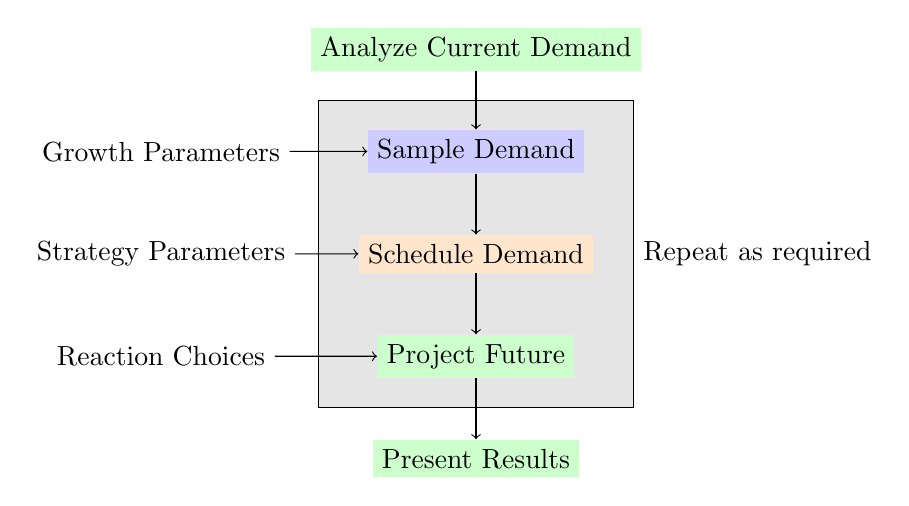
\begin{tikzpicture}[xscale=2,yscale=1.3]
  \draw[fill=black!10] (0,1.5) rectangle (2,4.5);
  \node[right] at (2,3) {Repeat as required};
  \node[fill=green!20] (analyse) at (1,5) {Analyze Current Demand};
  \node[fill=blue!20] (sample) at (1,4) {Sample Demand};
  \node (increase) at (-1,4) {Growth Parameters};
  \node (params) at (-1,3) {Strategy Parameters};
  \node (reaction) at (-1,2) {Reaction Choices};
  \node[fill=orange!20] (schedule) at (1,3) {Schedule Demand};
  \node[fill=green!20] (project) at (1,2) {Project Future};
  \node[fill=green!20] (present) at (1,1) {Present Results};
  \draw[->] (analyse) -- (sample);
  \draw[->] (increase) -- (sample);
  \draw[->] (sample) -- (schedule);
  \draw[->] (params) -- (schedule);
  \draw[->] (schedule) -- (project);
  \draw[->] (reaction) -- (project);
  \draw[->] (project) -- (present);
\end{tikzpicture}

\end{frame}

\begin{frame}
\frametitle{Demand Data (Not Public)}
\begin{tabular}{cc}
\shortstack{Received\\Per Day}&
\shortstack{Received\\Per Day of Week}\\
\includegraphics[width=4.5cm]{imagesoutpatient/referralsperday} &
\includegraphics[width=4.5cm]{imagesoutpatient/referralsdayofweek}
\end{tabular}

{\small
\begin{itemize}
\item Fitting distributions
\begin{itemize}
\item Poisson, not good fit
\item Negative Binomial
\end{itemize}
\item Limited Seasonality (unlike Emergency Department)
\end{itemize}
}
\end{frame}

% \begin{frame}
% \frametitle{Growth Parameters}
% \begin{itemize}
% \item Short/medium-term horizon (12-24 months)
% \begin{itemize}
% \item Keep demand constant
% \item Increase with historical rates
% \item Consider regional population increase 
% \end{itemize}
% \item More Complex:
% \begin{itemize}
% \item Age structure, birth rates
% \item More appropriate for long-term demand forecast
% \end{itemize}
% \end{itemize}
% \end{frame}

\begin{frame}
\frametitle{Waitlist/Clinic Model}
\scalebox{0.45}{
  \begin{tikzpicture}
    \node at (0,12) {Clinicians};
    \node at (7,12) {Clinic};
    \node at (14,12) {Waitlist};
\node[fill=red!10] (smyth) at (0,9) {Dr A}; 
\node[fill=red!10, below = 2 cm of smyth] (mahesh)  {Dr B}; 
\node[fill=red!10, below = 2 cm of mahesh] (lang)  {Dr C}; 
\node[fill=red!10, below = 2 cm of lang] (skinner)  {Dr D}; 
\node[fill=red!10, below = 2 cm of skinner] (donnelly)  {Dr E}; 
\node[fill=blue!10] (entcf) at (7,10) {ENTCF}; 
\node[fill=blue!10, below = 0.5 cm of entcf ] (entds)  {ENT A}; 
\node[fill=blue!10, below = 0.5 cm of entds ] (entdx)  {ENTAA}; 
\node[fill=blue!10, below = 0.5 cm of entdx ] (entel)  {ENT C}; 
\node[fill=blue!10, below = 0.5 cm of entel ] (entmh)  {ENT B}; 
\node[fill=blue!10, below = 0.5 cm of entmh ] (entms)  {ENT D}; 
\node[fill=blue!10, below = 0.5 cm of entms ] (entmt)  {ENT E}; 
\node[fill=blue!10, below = 0.5 cm of entmt ] (entpc)  {ENTPC}; 
\node[fill=blue!10, below = 0.5 cm of entpc ] (entsl)  {ENTSL}; 
\node[fill=blue!10, below = 0.5 cm of entsl ] (entvc)  {ENTVC}; 
\node[fill=blue!10, below = 0.5 cm of entvc ] (race)  {RACE}; 
\node[fill=blue!10, below = 0.5 cm of race ] (skcl)  {HNL}; 
\node[fill=blue!10, below = 0.5 cm of skcl ] (thyr)  {THYR}; 
\node[fill=green!10] at (14,10) (cystic) {Cystic F.};
\node[fill=green!10, below= 0.5 cm of cystic]  (smyth_wl) {Dr A WL};
\node[fill=green!10, below= 0.5 cm of smyth_wl]  (lang_wl) {Dr C WL}; 
\node[fill=green!10, below= 0.5 cm of lang_wl]  (ent) {ENT General}; 
\node[fill=green!10, below= 0.5 cm of ent]  (mahesh_wl) {Dr B WL}; 
\node[fill=green!10, below= 0.5 cm of mahesh_wl]  (skinner_wl) {Dr D WL}; 
\node[fill=green!10, below= 0.5 cm of skinner_wl]  (donnelly_wl) {Dr E WL}; 
\node[fill=green!10, below= 0.5 cm of donnelly_wl]  (paed) {ENT Paedicatrics}; 
\node[fill=green!10, below= 0.5 cm of paed]  (speech) {Speech \& Language}; 
\node[fill=green!10, below= 0.5 cm of speech]  (voice) {Voice}; 
\node[fill=green!10, below= 0.5 cm of voice]  (rapid) {ENT Rapid Access}; 
\node[fill=green!10, below= 0.5 cm of rapid]  (lesion) {Head Neck Lesions}; 
\node[fill=green!10, below= 0.5 cm of lesion]  (thyroid) {Thyroid}; 
\draw[] (smyth) -- (entcf); 
\draw[] (smyth) -- (entds); 
\draw[] (smyth) -- (entdx); 
\draw[] (lang) -- (entel); 
\draw[] (lang) -- (entpc); 
\draw[] (lang) -- (entsl); 
\draw[] (lang) -- (entvc); 
\draw[] (lang) -- (thyr); 
\draw[] (mahesh) -- (entmh); 
\draw[] (skinner) -- (entms); 
\draw[] (skinner) -- (entsl); 
\draw[] (skinner) -- (thyr); 
\draw[] (donnelly) -- (entmt); 
\draw[] (donnelly) -- (race); 
\draw[] (donnelly) -- (skcl); 
\draw[] (entcf) -- (cystic); 
\draw[] (entds) -- (smyth_wl); 
\draw[] (entdx) -- (smyth_wl); 
\draw[] (entel) -- (lang_wl); 
\draw[] (entds) -- (ent); 
\draw[] (entdx) -- (ent); 
\draw[] (entel) -- (ent); 
\draw[] (entmh) -- (ent); 
\draw[] (entms) -- (ent); 
\draw[] (entmt) -- (ent); 
\draw[] (entmh) -- (mahesh_wl); 
\draw[] (entms) -- (skinner_wl); 
\draw[] (entmt) -- (donnelly_wl); 
\draw[] (entpc) -- (paed); 
\draw[] (entsl) -- (speech); 
\draw[] (entvc) -- (voice); 
\draw[] (race) -- (rapid); 
\draw[] (skcl) -- (lesion); 
\draw[] (thyr) -- (thyroid); 
\draw[dotted] (entel) -- (rapid); 
\draw[dotted] (entms) -- (rapid); 
\draw[] (skinner) -- (entvc);
\end{tikzpicture}
}

\end{frame}


\begin{frame}
\frametitle{Learning Capacity from Historical Data}
\includegraphics[width=10cm]{imagesoutpatient/samplecliniccalendar}
{\small
\begin{itemize}
\item Repeat frequency
\item Capacity
\item Cancellation frequency
\item Replacement clinics
\end{itemize}
}
\end{frame}

\begin{frame}
\frametitle{Optimization Problem}
\begin{itemize}
\item Assign waiting patients to slots in clinics
\item Use appropriate clinic for given patient
\item Make appointments $k_p$ days in advance
\item Free and reuse slots when patients cancel
\item Reschedule patients when clinic cancelled
\item Do not change appointments otherwise
\item Reserve $u$ slots for urgent cases
\item Solved for each day
\end{itemize}
\end{frame}

\begin{frame}
\frametitle{Waitlist Actions}
\scalebox{0.55}{
  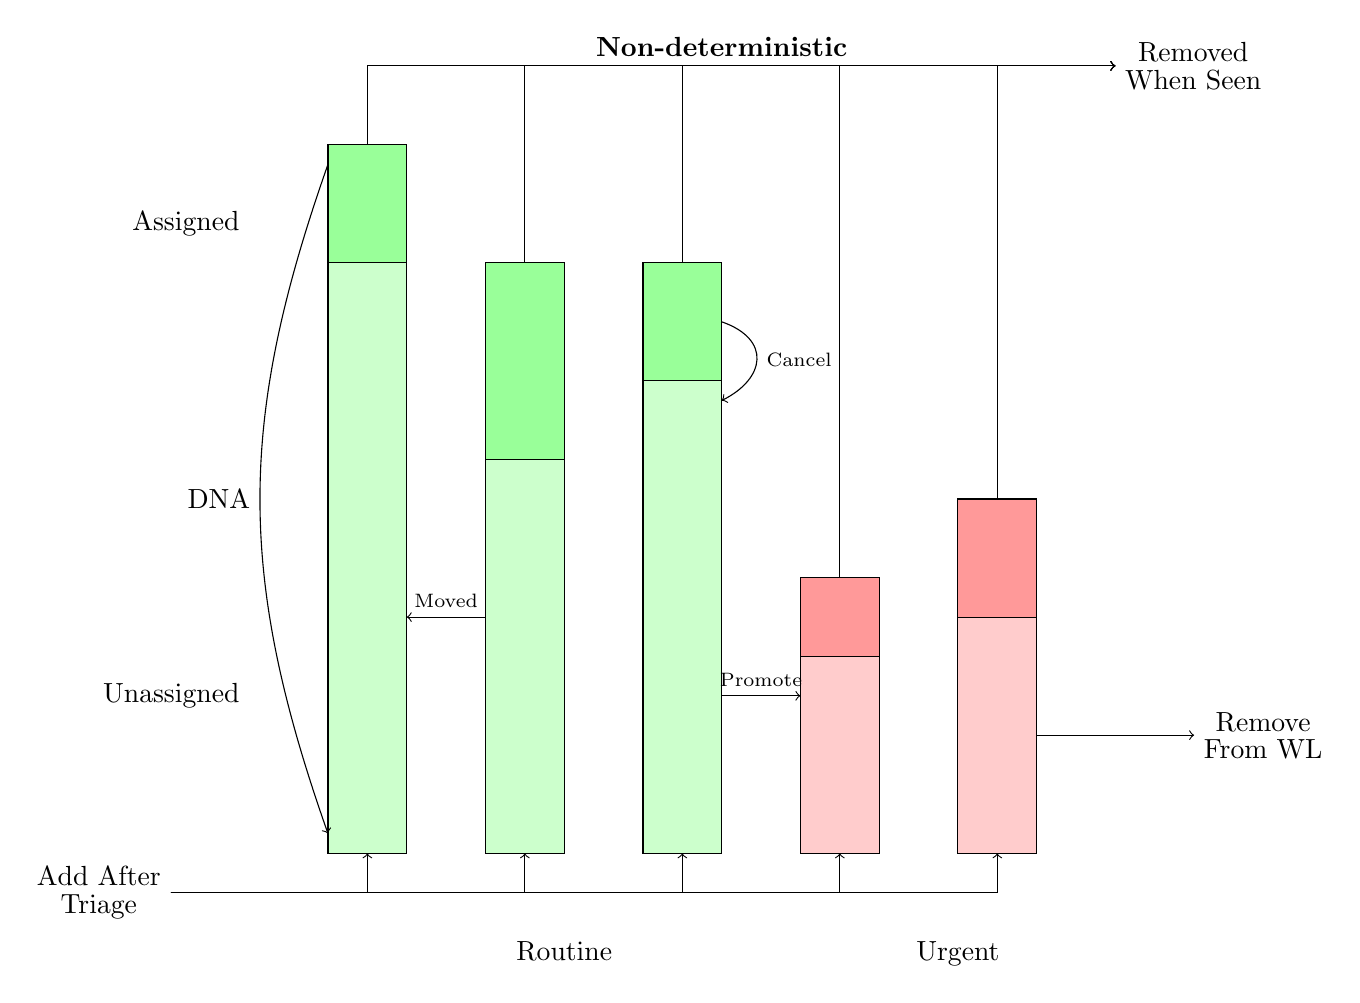
\begin{tikzpicture}[xscale=1,yscale=0.5]
  \draw[fill=green!20] (0,0) rectangle (1,15);
  \draw[fill=green!40] (0,15) rectangle (1,18);
  \draw[fill=green!20] (2,0) rectangle (3,10);
  \draw[fill=green!40] (2,10) rectangle (3,15);
  \draw[fill=green!20] (4,0) rectangle (5,12);
  \draw[fill=green!40] (4,12) rectangle (5,15);
  \draw[fill=red!20] (6,0) rectangle (7,5);
  \draw[fill=red!40] (6,5) rectangle (7,7);
  \draw[fill=red!20] (8,0) rectangle (9,6);
  \draw[fill=red!40] (8,6) rectangle (9,9);
  \node[below] at (3,-2) {Routine};
  \node[below] at (8,-2) {Urgent};
  \node[left] at (-1,4) {Unassigned};
  \node[left] at (-1,16) {Assigned};
  \draw[->] (-2,-1) -- (0.5,-1) -- (0.5,0);
  \draw[->] (-2,-1) -- (2.5,-1) -- (2.5,0);
  \draw[->] (-2,-1) -- (4.5,-1) -- (4.5,0);
  \draw[->] (-2,-1) -- (6.5,-1) -- (6.5,0);
  \draw[->] (-2,-1) -- (8.5,-1) -- (8.5,0);
  \node[left] at (-2,-1) {\shortstack{Add After\\Triage}};
  \draw[->] (0.5,18) -- (0.5,20) -- (10,20);
  \draw[->] (2.5,15) -- (2.5,20) -- (10,20);
  \draw[->] (4.5,15) -- (4.5,20) -- (10,20);
  \draw[->] (6.5,7) -- (6.5,20) -- (10,20);
  \draw[->] (8.5,9) -- (8.5,20) -- (10,20);
  \node[right] at (10,20) {\shortstack{Removed\\When Seen}};
  \node[above] at (5,20) {\textbf{Non-deterministic}};
  \draw[->] (0,17.5) to [out=260,in=100] node[left] {DNA} (0,0.5);
  \draw[->] (5,13.5) to [out=325,in=45] node[right] {\scriptsize Cancel} (5,11.5);
  \draw[->] (2,6) -- node[above] {\scriptsize Moved} (1,6);
  \draw[->] (5,4) -- node[above] {\scriptsize Promote} (6,4);
  \draw[->] (9,3) --  (11,3);
  \node[right] at (11,3) {\shortstack{Remove\\From WL}};
\end{tikzpicture}
}

\end{frame}

\begin{frame}
\frametitle{Clinic Allocation}
\scalebox{0.6}{
  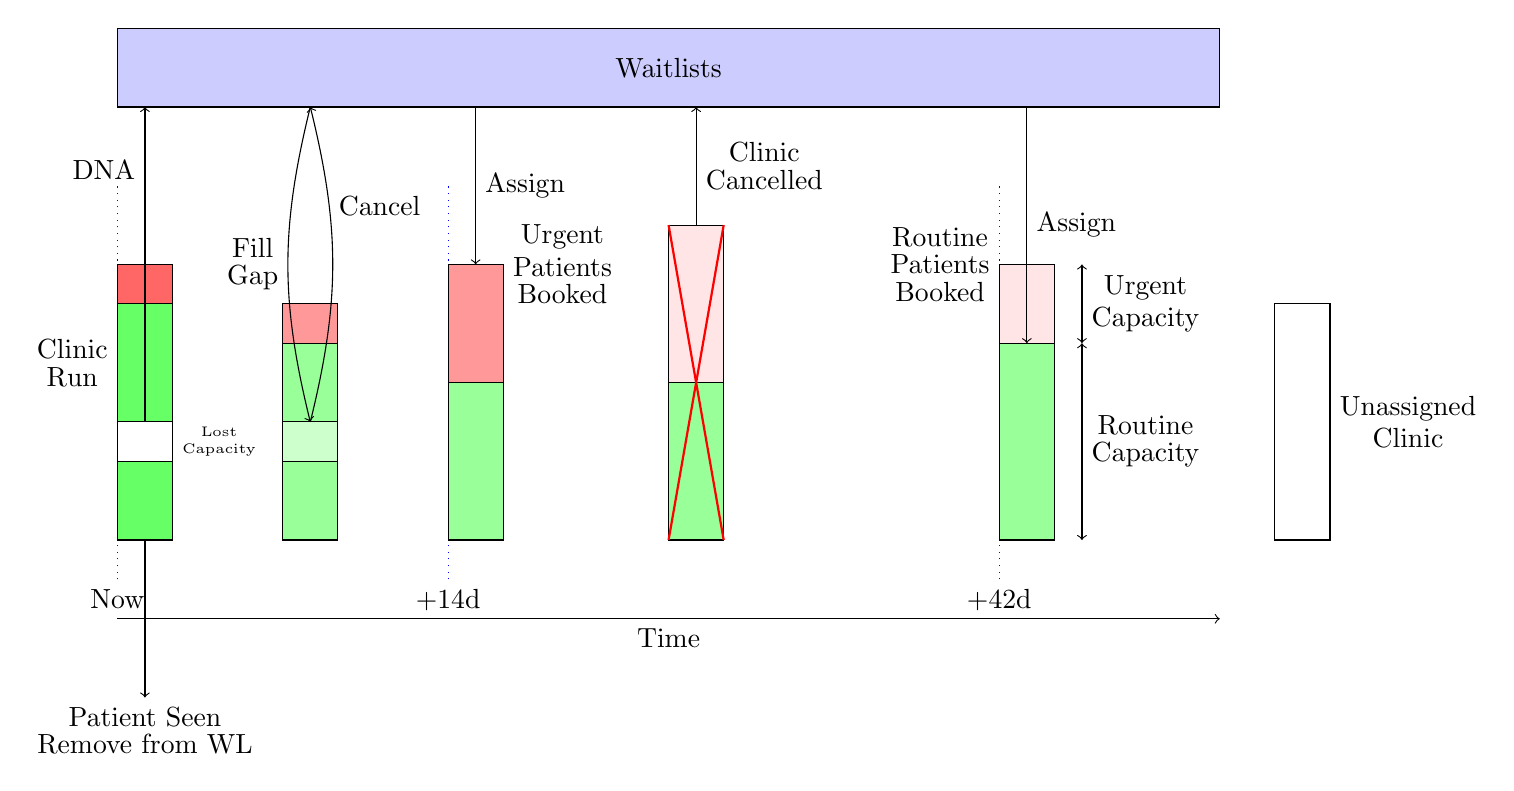
\begin{tikzpicture}[xscale=0.7,yscale=0.5]
    \draw[->](0,-2) --node[below] {Time} (20,-2);
    \draw[dotted,blue] (0,-1) -- (0,9);
    \draw[dotted,blue] (6,-1) -- (6,9);
    \draw[dotted,blue] (16,-1) -- (16,9);
    \node[below] at (0,-1) {Now};
    \node[below] at (6,-1) {+14d};
    \node[below] at (16,-1) {+42d};
    
    \draw[fill=green!60] (0,0) rectangle (1,6);
    \draw[fill=red!60] (0,6) rectangle (1,7);
    \node[left] at (0,4.5) {\shortstack{Clinic\\Run}};
    
    \draw[fill=green!40] (3,0) rectangle (4,5);
    \draw[fill=red!40] (3,5) rectangle (4,6);
    

    \draw[fill=green!40] (6,0) rectangle (7,4);
    \draw[fill=red!40] (6,4) rectangle (7,7);
    \node [right] at (7,7) {\shortstack{Urgent\\Patients\\Booked}};

    \draw[fill=green!40] (10,0) rectangle (11,4);
    \draw[fill=red!10] (10,4) rectangle (11,8);

    \draw[fill=green!40] (16,0) rectangle (17,5);
    \draw[fill=red!10] (16,5) rectangle (17,7);
    \node [left] at (16,7) {\shortstack{Routine\\Patients\\Booked}};

    \draw[fill=none,draw=black] (21,0) rectangle (22,6);
    \node[right] at (22,3) {\shortstack{Unassigned\\Clinic}};

    \draw[<->] (17.5,0) -- node[right] {\shortstack{Routine\\Capacity}} (17.5,5);
    \draw[<->] (17.5,5) -- node[right] {\shortstack{Urgent\\Capacity}} (17.5,7);

    \draw[fill=blue!20] (0,11) rectangle (20,13);
    \node at (10,12) {Waitlists};

    \draw[->] (16.5,11) -- node[right] {Assign} (16.5,5);
    \draw[->] (6.5,11) -- node[right] {Assign} (6.5,7);
    \draw[fill=white,draw=black] (0,2) rectangle(1,3);
    \node[right] at (1,2.5) {\tiny\shortstack{Lost\\Capacity}};
    \draw[->] (0.5,3) -- node[pos=0.8,left] {DNA} (0.5,11);
    \draw[->] (0.5,0) -- (0.5,-4);
    \node[below] at (0.5,-4) {\shortstack{Patient Seen\\Remove from WL}};

    \draw[fill=green!20] (3,2) rectangle (4,3);
    \draw[<-] (3.5,11) to [out=280,in=80] node[pos=0.3,right] {Cancel} (3.5,3);
    \draw[<-] (3.5,3) to [out=100,in=260] node[left] {\shortstack{Fill\\Gap}} (3.5,11);

    \draw[red,thick] (10,0) -- (11,8);
    \draw[red,thick] (11,0) -- (10,8);
    \draw[->,black] (10.5,8) -- node[right] {\shortstack{Clinic\\Cancelled}} (10.5,11);
  \end{tikzpicture}
}

\end{frame}

\subsection{Results}
\begin{frame}
\frametitle{Baseline Analysis, Management View}
\includegraphics[width=10.5cm]{imagesoutpatient/baseline}
\end{frame}

\begin{frame}
\frametitle{Scenario: Balance Patients Between Hospitals}
\includegraphics[width=10.5cm]{imagesoutpatient/balanced}
\end{frame}

\begin{frame}
\frametitle{Scenario: Reduce DNA (Did not attend) to 5\%}
\includegraphics[width=10.5cm]{imagesoutpatient/dna5percent}
\end{frame}

\begin{frame}
\frametitle{Scenario: Add Capacity}
\includegraphics[width=10.5cm]{imagesoutpatient/drnew}
\end{frame}

% \begin{frame}
% \frametitle{Scenario: Add More Capacity}
% \includegraphics[width=10.cm]{imagesoutpatient/drnew2}
% \end{frame}

\subsection{Summary}
% \begin{frame}
% \frametitle{Status}
% \begin{textblock*}{4cm}(11cm,4cm)
% \includegraphics[width=4cm]{imagesoutpatient/stimulai.png}
% \end{textblock*}

% \begin{itemize}
% \item Initially developed with industrial partner
% \item Tested and evaluated at hospital
% \item Actual data used, but manual feed
% \item Startup company Stimul.AI to commercialize solution
% \end{itemize}
% \end{frame}

% \begin{frame}
% \frametitle{The Need is Still There}
% \includegraphics[width=7cm]{imagesoutpatient/newoutpatientswaitingaug2018}
% \end{frame}

%% \begin{frame}
%% \frametitle{Dashboard}
%% \includegraphics[width=10cm]{imagesoutpatient/ntpf}
%% \end{frame}

%% \begin{frame}
%% \frametitle{Key Factor: Return/New Ratio}
%% \includegraphics[width=10cm]{imagesoutpatient/kpireturnewratio}
%% \end{frame}

\begin{frame}
\frametitle{Summary}
\begin{itemize}
\item Presented case study from Irish health system
\item Strategy for outpatient appointments
\item Mix of analytics, simulation, and optimization
\item Nation-wide analysis of available data
\item What-if tool for selected departments
\end{itemize}
\end{frame}


}
\mode<all>{\section{Elevator Maintenance Planning and Scheduling}

\begin{frame}
\frametitle{Joint work with...}
\begin{itemize}
\item Mark Antunes, Vincent Armant, Kenneth N. Brown, Gabriel G. Castane, Daniel Desmond,
Guillaume Escamocher, Michele Garraffa, Anne-Marie George, Diarmuid Grimes, Mike O'Keefe, Yiqing Lin,
Barry O'Sullivan, Cemalettin Ozturk, Luis Quesada, Mohamed Siala, Helmut Simonis
and Nic Wilson
\end{itemize}
\end{frame}

\subsection{Introduction}

\begin{frame}
\frametitle{Real World Problem}
\begin{itemize}
\item Manufacturing Industry, after sales support
\item Maintenance is crucial for safety/availability of product
\item Preventive/Predictive/Reactive Maintenance influence each other
\item  How to organize service, what to do?
\end{itemize}
\end{frame}

\begin{frame}
\frametitle{Research Challenge}
\begin{itemize}
\item How to plan/schedule if events interrupt planned work
\item How to use predictive maintenance to avoid problems before they occur
\item What is the right problem decomposition?
\end{itemize}
\end{frame}

% \begin{frame}
% \frametitle{Using Industrial Problems as Research Challenge}
% \begin{itemize}
% \item Trying to make three points:
% \begin{itemize}
% \item This is an important industrial problem
% \item There is an interesting research question to be solved
% \item We are making a contribution to solving the problem
% \end{itemize}
% \item Highlighting some of the challenges
% \begin{itemize}
% \item Private data
% \item Scalability
% \item Managing expectations
% \end{itemize}
% \end{itemize}
% \end{frame}

\begin{frame}
\frametitle{Travelling Repair Person (TRP)}
\begin{itemize}
\item Providing service for devices at customer premises
\item Planned preventive maintenance and testing, regular visits
\item Technicians travel to multiple, but few customers per day
\item Unplanned repair work after faults, response-time critical
\item Service times quite variable
\item Impact of skills and local knowledge
\end{itemize}
\end{frame}

% \begin{frame}
% \frametitle{Compared to Other Service Planning Problems}
% \begin{itemize}
% \item Stationary technician, moving customers
% \begin{itemize}
% \item Example: car tune-up
% \item Preventive, planned work
% \item Either a queuing or scheduling problem
% \end{itemize}
% \item Moving customer, moving technician
% \begin{itemize}
% \item Road side assistance
% \item Reactive, unplanned work
% \item On-line dispatching, pre-positioning
% \end{itemize}
% \item Moving technician, stationary customers
% \begin{itemize}
% \item Example: cable installation, photocopier repair
% \item Mainly reactive, sometimes planned work as well
% \item Routing and scheduling aspects
% \end{itemize}
% \end{itemize}
% \end{frame}

\begin{frame}
\frametitle{Why is this important? (1)}
\includegraphics[width=11cm]{imagesfieldservice/southchina}
\end{frame}

\begin{frame}
\frametitle{Why is this important? (2)}
\includegraphics[width=11cm]{imagesfieldservice/schindlerjapan}

Source: \includegraphics[width=2cm]{imagesfieldservice/reuters}

\end{frame}

\begin{frame}
\frametitle{Why is this important? (3)}
\includegraphics[width=8cm]{imagesfieldservice/hancock}
\includegraphics[width=3cm]{imagesfieldservice/John_Hancock_Center_2019}

{\tiny Source: By Chris6d - Own work, CC BY-SA 4.0, https://commons.wikimedia.org/w/index.php?curid=78201640}
\end{frame}

% \begin{frame}
% \frametitle{Why is this important? (4)}
% \includegraphics[width=7.5cm]{imagesfieldservice/ontario}
% \end{frame}


% \begin{frame}
% \frametitle{TRP Compared to Other Combinatorial Problems}
% 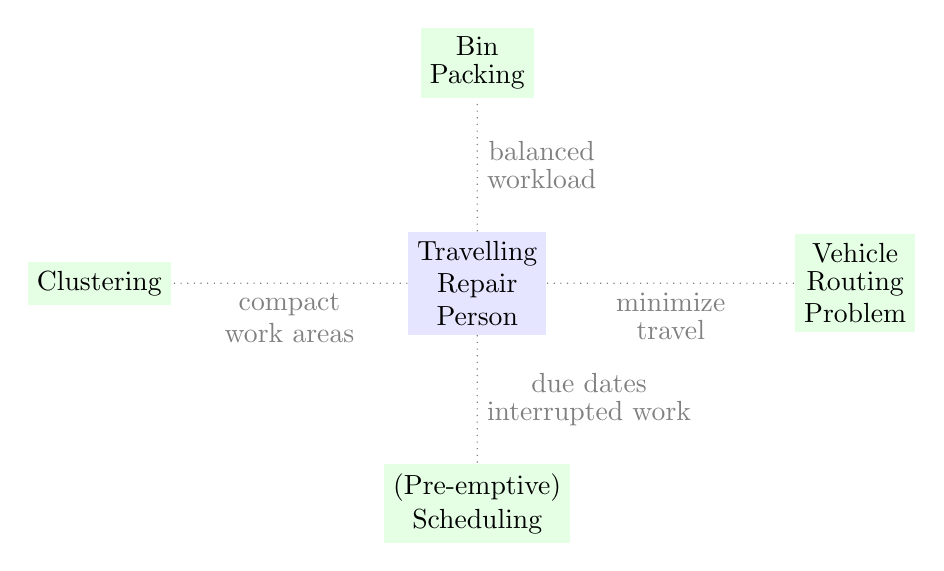
\begin{tikzpicture}[xscale=2.4,yscale=1.4]
  \node[fill=blue!10] (trp) at (2,2) {\shortstack{Travelling\\Repair\\Person}};
  \node[fill=green!10] (bin) at (2,4) {\shortstack{Bin\\Packing}};
  \node[fill=green!10] (clustering) at (0,2) {Clustering};
  \node[fill=green!10] (vrp) at (4,2) {\shortstack{Vehicle\\Routing\\Problem}};
  \node[fill=green!10] (scheduling) at (2,0) {\shortstack{(Pre-emptive)\\Scheduling}};
  \draw[gray,dotted] (trp) -- node[right] {\shortstack{balanced\\workload}} (bin);
  \draw[gray,dotted] (trp) -- node[below] {\shortstack{compact\\work areas}}(clustering);
  \draw[gray,dotted] (trp) -- node[below] {\shortstack{minimize\\travel}} (vrp);
  \draw[gray,dotted] (trp) -- node[right] {\shortstack{due dates\\interrupted work}} (scheduling);
\end{tikzpicture}

% \end{frame}

% \begin{frame}
% \frametitle{TRP - Interesting Research Problem}
% \begin{itemize}
% \item Combines elements of multiple combinatorial problems
% \item Hard constraints, multiple cost element
% \item Stochastic events are core part of problem
% \end{itemize}
% \end{frame}

% \begin{frame}
% \frametitle{Key Research Challenge}
% \begin{itemize}
% \item Use combination of Optimization and Simulation to model and solve the TRP
% \item Optimization
% \begin{itemize}
% \item Good for global cost model
% \item Detailed constraints of problem
% \item (-) Does not easily deal with unplanned work
% \end{itemize}
% \item Simulation
% \begin{itemize}
% \item Good for modelling individual actors
% \item Understanding impact of stochastic changes
% \item (-) No global view of problem
% \end{itemize}
% \end{itemize}
% \end{frame}

\subsection{Our Contribution}

\begin{frame}
\frametitle{High-level View}
\includegraphics[width=11cm]{imagesfieldservice/highleveloverview}
\begin{itemize}
\item Optimizer deals with planning, load balancing, efficient schedules
\item Simulator explores how to react to changes
\item Simulator also provides one result as assumed reality
\end{itemize}
\end{frame}

\begin{frame}
\frametitle{Optimizer Design}
\begin{itemize}
\item Infeasible to build homogenuous model for complete problem
\item Added business process constraint
\begin{itemize}
\item Technicians should be responsible for ``their'' buildings
\item Improves service quality
\item Customers see familiar face
\end{itemize}
\item All work in one building should be performed by the same engineer, if possible
\item Engineers should be assigned compact areas of work
\item Balanced workload within the same depot
\end{itemize}
\end{frame}

\begin{frame}
\frametitle{Optimizer Decomposition}
\includegraphics[width=10.5cm]{imagesfieldservice/decomposition}
\end{frame}

\begin{frame}
\frametitle{Clustering and Depot Assignment}
\includegraphics[width=11cm]{imagesfieldservice/depotassignment}
\end{frame}

% \begin{frame}
% \frametitle{Routes and Trips}
% \includegraphics[width=8.5cm]{imagesfieldservice/toursinroutes}
% \end{frame}

% \begin{frame}
% \frametitle{Actual Data: Workload and Callbacks as Treemap}
% \includegraphics[width=11cm]{imagesfieldservice/treemap}
% \end{frame}

% \begin{frame}
% \frametitle{Actual Data: Mix of Urban and Rural Customers}
% \includegraphics[width=11cm]{imagesfieldservice/mapcanada}
% \end{frame}

% \begin{frame}
% \frametitle{Actual Data: Balancing Workload Within Depots}
% \includegraphics[width=11cm]{imagesfieldservice/barchartbalanced}
% \end{frame}

\begin{frame}
\frametitle{Scheduling: One Day of Monthly Plan}
\includegraphics[width=11cm]{imagesfieldservice/schedule}
\end{frame}

\begin{frame}
\frametitle{Methods Used}
\begin{description}
\item[Clustering] Connected components on generated graph
\item[Routing] Which places to visit in one trip
\begin{itemize}
\item Core MIP Model
\item Iterative MIP inside Clustering
\item Two stage grouping of locations to reduce expected travel
\item Local Search
\end{itemize}
\item[Scheduling] Dynamic Programming and Set Partitioning
\end{description}
\end{frame}

%% \begin{frame}
%% \frametitle{Integration with Simulator, First Day}
%% \includegraphics[width=11cm]{imagesfieldservice/integration1}
%% \end{frame}

%% \begin{frame}
%% \frametitle{Integration with Simulator, Next Day}
%% \includegraphics[width=11cm]{imagesfieldservice/integration2}
%% \end{frame}

% \begin{frame}
% \frametitle{Integration with Simulator, First Day}
% \includegraphics[width=8cm]{imagesfieldservice/dayscheduler1}
% \end{frame}

% \begin{frame}
% \frametitle{Integration with Simulator, Next Day}
% \includegraphics[width=8cm]{imagesfieldservice/dayscheduler2}
% \end{frame}

\begin{frame}
\frametitle{Simulator Process Modelling}
\includegraphics[width=11cm]{imagesfieldservice/processmodelling}
\end{frame}

\begin{frame}
\frametitle{Dealing with Unplanned Callbacks}
\includegraphics[width=10cm]{imagesfieldservice/callbacks}
\begin{itemize}
\item Who is dealing with the callback?
\item How to adjust the schedule after callback?
\end{itemize}
\end{frame}

\subsection{Evaluation}

\begin{frame}
\frametitle{Use Cases}
\begin{itemize}
\item Compare variants of problem to understand impact of changes
\item Examples
\begin{itemize}
\item Where to place depots and their area? 
\item How many technicians are needed in which depots?
\item Should technicians do both planned and unplanned work?
\item When is overtime the better choice?
\end{itemize}
\end{itemize}
\end{frame}

\begin{frame}
\frametitle{Scenario Evaluation: KPI Comparison}
\includegraphics[width=9cm]{imagesfieldservice/scenarioevaluation}
\end{frame}

\begin{frame}
\frametitle{Scenario Evaluation: Qualitative Differences}
\includegraphics[width=10cm]{imagesfieldservice/scheduledactualwork}
\begin{itemize}
\item On left, each point shows the outcome of one month of optimization+simulation
\item On right, compare outcomes for different scenarios, clear clustering of results
\end{itemize}
\end{frame}

% \begin{frame}
% \frametitle{Scenario Evaluation: Drill-down to Details}
% \includegraphics[width=11cm]{imagesfieldservice/detailsoverview}
% \end{frame}

% \begin{frame}
% \frametitle{Scenario Evaluation: Further Drill-down}
% \includegraphics[width=9cm]{imagesfieldservice/detailday}
% \end{frame}

\subsection{Challenges}

\begin{frame}
\frametitle{Challenges: Data}
\begin{itemize}
\item We need company internal data to understand problem
\item Problem for publication, for continued work
\item Open data as alternatives
\begin{itemize}
\item New York City
\begin{itemize}
\item 76,000 elevators with locations
\end{itemize}
\item Toronto, ON
\begin{itemize}
\item 40,000 elevators
\item Inspection dates, outcomes
\item Accident and injury reports
\end{itemize}
\end{itemize}
\end{itemize}
\end{frame}

\begin{frame}
\frametitle{Challenges: Scalability}
\includegraphics[width=11cm]{imagesfieldservice/simulatorscalability}
\end{frame}

\begin{frame}
\frametitle{Challenges: Tools and Results}
\begin{itemize}
\item We provide research and experimental software
\item \textbf{Not} a solution
\item End-user would like applicable results
\item Managing expectations is important
\end{itemize}
\end{frame}

% \begin{frame}
% \frametitle{What I did not talk about}
% \begin{itemize}
% \item Preferences and Incentives
% \begin{itemize}
% \item Retention of personnel
% \item Optimize while taking preferences into account
% \end{itemize}
% \item Elevator health
% \begin{itemize}
% \item If you don't do the maintenance, then elevators will fail
% \end{itemize}
% \item Condition Based Maintenance
% \begin{itemize}
% \item You can predict some of the failures and prevent them
% \end{itemize}
% \end{itemize}
% \end{frame}


\begin{frame}
\frametitle{Conclusions}
\begin{itemize}
\item We presented the Travelling Repair Person Problem
\item Important as an industrial problem
\item Interesting as a research challenge
\item We use combination of optimization and simulation to deal with novel properties of problem
\item System transferred to customer in 2019
\end{itemize}
\end{frame}
}
%\mode<all>{\section{CAT Constraint Acquisition}

\begin{frame}
\frametitle{Based on previous work with}
\begin{textblock*}{6cm}(9cm,1cm)
\includegraphics[width=6cm]{imagescat/zenodo.png}
\end{textblock*}

\begin{itemize}
\item N. Beldiceanu, IMT Atlantique
\item M. Carlsson, SICS
\end{itemize}
\vspace{2cm}
PTHG21 Challenge co-organized with E. Freuder
\end{frame}

\subsection{Introduction}

\begin{frame}
\frametitle{Industrial Problem}
\begin{itemize}
\item Industry
\item Optimization Projects are hard to manage
\item Skilled experts are not easily found
\item Communication between domain experts and programmers key
\item Easy to miss key constraint during design 
\end{itemize}
\end{frame}

\begin{frame}
\frametitle{Research Challenge}
\begin{itemize}
\item How can we make optimization more accessible?
\item Lower barriers to entry
\item or, make existing experts more productive
\item Bridge gap between application domain and abstract optimization concepts
\end{itemize}
\end{frame}

\begin{frame}
\frametitle{Take-Away Points}
\begin{itemize}
\item Constraint Acquisition provides a way to learn constraint model from data
\item Questions about use cases
\item Transferable, executable models
\item Common benchmark set: PTHG21 Challenge
\item CAT System shows feasibility of approach
\end{itemize}
\end{frame}

\begin{frame}
\frametitle{Background}
\begin{itemize}
\item ASSISTANT project (EU H2020, ICT-38 project, \url{https://assistant-project.eu/})
\item Constraint Acquisition part of WP 4
\item Making Constraint Acquisition relevant in real world, scheduling setting
\item Based on case studies from Siemens Energy and Atlas Copco
\end{itemize}
\includegraphics[width=5cm]{imagescat/assistantpartners}
\end{frame}

\subsection{Solution Approach}
\begin{frame}
\frametitle{Constraint Acquisition - What is it?}
\begin{itemize}
\item Learn Constraint Models from data
\begin{itemize}
\item Given positive and negative examples ("Passive")
\item Asking questions to user ("Active")
\end{itemize}
\item Useful to
\begin{itemize}
\item Understand problem
\item Classify new examples as solutions or non-solutions
\item Use generated model to find solutions 
\end{itemize}
\end{itemize}
\end{frame}

% \begin{frame}
% \frametitle{Literature}
% \begin{itemize}
% \item Christian Bessiere, Frédéric Koriche, Nadjib Lazaar, Barry O'Sullivan:
% Constraint acquisition. Artif. Intell. 244: 315-342 (2017)
% \item Remi Coletta, Christian Bessière, Barry O'Sullivan, Eugene C. Freuder, Sarah O'Connell, Joël Quinqueton:
% Semi-automatic Modeling by Constraint Acquisition. CP 2003: 812-816
% \item Christian Bessiere, Remi Coletta, Frédéric Koriche, Barry O'Sullivan:
% Acquiring Constraint Networks Using a SAT-based Version Space Algorithm. AAAI 2006: 1565-1568
% \item Mohit Kumar, Stefano Teso, Luc De Raedt:
% Acquiring Integer Programs from Data. IJCAI 2019: 1130-1136
% \item Nicolas Beldiceanu, Helmut Simonis:
% A Model Seeker: Extracting Global Constraint Models from Positive Examples. CP 2012: 141-157

% \end{itemize}
% \end{frame}

% \begin{frame}
% \frametitle{State of the Art Discussion}
% \begin{itemize}
% \item Many different approaches
% \item Not based on a common use case
% \item Comparison of results difficult
% \item PTHG21 Challenge tried to shape discussion
% \end{itemize}
% \end{frame}

% \begin{frame}<1>[label=zooms]
  \frametitle{Example: Sudoku}
  \framezoom<1><2>(0cm,0cm)(4.2cm,2.7cm)
  \framezoom<1><3>(10.3cm,0cm)(4.7cm,2.5cm)
  \framezoom<1><4>(2.6cm,2.8cm)(10.2cm,3.9cm)
  \scalebox{0.4}{
  \begin{tikzpicture}[xscale=5,yscale=3,
  inputdata/.style={fill=insight-burntorange!10,draw=black,rounded corners},
program/.style={fill=insight-lime!20,draw=black!30},
documents/.style={fill=insight-royalblue!20,draw=black!30,rounded corners,drop shadow},
positive/.style={fill=insight-aqua!20,draw=black!30,rounded corners,drop shadow},
negative/.style={fill=insight-burntorange!20,draw=black!30,rounded corners,drop shadow},
test/.style={fill=insight-plum!20,draw=black!30,rounded corners,drop shadow},
extrasolution/.style={fill=insight-yellow!20,draw=black!30,rounded corners,drop shadow},
document/.style={fill=insight-royalblue!20,draw=black,rounded corners}]

    \draw[draw,rounded corners] (0.7,1.5) rectangle (1.3,3.5);
    \node[below] at(1,1.5) {\LARGE Instance 1};
    
    \draw[draw,rounded corners] (1.4,1.5) rectangle (2.7,3.5);
    \node[below] at(2,1.5) {\LARGE Instance 2};
    
    \node[positive,label={90:Solution}] at (1,3)
      {\scriptsize  \begin{tabular}{cccc}1&3&2&4\\
2&4&1&3\\
3&1&4&2\\
4&2&3&1\\
\end{tabular}};

    \node[negative,label={90:Nonsolution}] at (1,2)         
{\scriptsize \begin{tabular}{cccc}
2&4&3&3\\
1&3&4&2\\
4&2&3&1\\
3&1&2&4\\
\end{tabular}};

    \node[positive] at (2,3)
{\tiny \begin{tabular}{*{9}{c}}
9&5&7&6&4&8&3&2&1\\
4&8&3&1&5&2&6&9&7\\
1&6&2&9&7&3&5&8&4\\
5&2&1&8&3&6&4&7&9\\
3&9&6&4&1&7&2&5&8\\
7&4&8&5&2&9&1&3&6\\
6&3&9&2&8&4&7&1&5\\
8&7&5&3&6&1&9&4&2\\
2&1&4&7&9&5&8&6&3\\
\end{tabular}};

    \node[negative] at (2,2)
{\tiny
\begin{tabular}{*{9}{c}}
7&1&3&6&9&2&8&5&4\\
8&8&2&5&7&4&1&3&9\\
5&5&4&1&8&3&7&2&6\\
3&3&9&4&6&1&5&8&7\\
6&7&1&8&2&5&9&4&3\\
5&8&5&9&3&7&2&6&1\\
8&3&6&2&5&8&5&7&5\\
2&5&7&3&4&9&6&1&8\\
1&4&8&7&5&7&3&9&2\\
\end{tabular}};

\node[program] (ca) at (3.5,2.5) {\Huge \shortstack{Constraint\\Acquisition}};
\node[program] (classify) at (3.5,1.5) {\Huge \shortstack{Classify\\Tests}};

\node[document,label={90:\LARGE Model}] (model) at (4.6,2.5) {\Huge\shortstack[l]{Each Row:\\ alldifferent\\Each Column:\\ alldifferent\\Each Block:\\ alldifferent}};
\node[program] (solver) at (5.5,2.5) {\Huge Solver};

\node[extrasolution,label={90:\LARGE Extra Solutions}] (extra) at (7,2.5)
     {\tiny \begin{tabular}{*{16}{c}}
16& 15& 14& 13& 12& 11& 10& 9& 8& 7& 6& 5& 4& 3& 2& 1\\
12& 11& 10& 9& 16& 15& 14& 13& 4& 3& 2& 1& 8& 7& 6& 5\\
8& 7& 6& 5& 4& 3& 2& 1& 16& 15& 14& 13& 12& 11& 10& 9\\
4& 3& 2& 1& 8& 7& 6& 5& 12& 11& 10& 9& 16& 15& 14& 13\\
15& 16& 13& 14& 11& 12& 9& 10& 7& 8& 5& 6& 3& 4& 1& 2\\
11& 12& 9& 10& 15& 16& 13& 14& 3& 4& 1& 2& 7& 8& 5& 6\\
7& 8& 5& 6& 3& 4& 1& 2& 15& 16& 13& 14& 11& 12& 9& 10\\
3& 4& 1& 2& 7& 8& 5& 6& 11& 12& 9& 10& 15& 16& 13& 14\\
14& 13& 16& 15& 10& 9& 12& 11& 6& 5& 8& 7& 2& 1& 4& 3\\
10& 9& 12& 11& 14& 13& 16& 15& 2& 1& 4& 3& 6& 5& 8& 7\\
6& 5& 8& 7& 2& 1& 4& 3& 14& 13& 16& 15& 10& 9& 12& 11\\
2& 1& 4& 3& 6& 5& 8& 7& 10& 9& 12& 11& 14& 13& 16& 15\\
13& 14& 15& 16& 9& 10& 11& 12& 5& 6& 7& 8& 1& 2& 3& 4\\
9& 10& 11& 12& 13& 14& 15& 16& 1& 2& 3& 4& 5& 6& 7& 8\\
5& 6& 7& 8& 1& 2& 3& 4& 13& 14& 15& 16& 9& 10& 11& 12\\
1& 2& 3& 4& 5& 6& 7& 8& 9& 10& 11& 12& 13& 14& 15& 16\\
\end{tabular}};


\node[below,test] (test2) at (2.5,0)
{\tiny
\begin{tabular}{cccc}
1&4&2&3\\
2&3&4&1\\
4&1&3&2\\
3&2&1&4\\
\end{tabular}}; 

    \node[below,test] (test3) at (3.5,0)
{\tiny
\begin{tabular}{*{9}{c}}
3&9&1&5&6&6&7&4&2\\
6&2&8&3&7&9&1&5&6\\
5&7&1&2&1&4&9&3&8\\
8&3&9&4&6&2&4&7&5\\
7&1&4&8&5&3&2&6&9\\
2&5&6&9&4&7&3&8&1\\
6&8&2&7&3&5&6&1&4\\
1&4&3&6&2&8&5&9&7\\
7&7&5&4&9&1&8&2&3\\
\end{tabular}};

    \node[below,test,label={270:Unseen Size}] (test4) at (5.5,0)
{\tiny
\begin{tabular}{*{16}{c}}
8&13&12&4&14&16&3&9&7&1&6&11&10&5&15&2\\
10&7&1&5&12&2&13&6&8&9&4&9&3&14&2&11\\
9&14&15&3&1&11&5&8&13&10&2&16&6&7&12&4\\
11&16&6&2&10&15&3&7&3&1&12&5&6&13&8&9\\
5&11&8&6&13&8&12&7&1&3&16&2&14&15&9&10\\
16&12&9&14&2&7&1&10&15&5&11&9&13&6&4&8\\
15&5&4&1&9&3&6&16&14&8&10&13&7&2&11&12\\
2&10&13&7&11&3&15&14&12&6&7&4&3&1&3&5\\
14&1&12&8&16&13&14&5&9&15&3&7&8&9&13&6\\
3&8&9&7&6&13&10&12&4&11&1&14&14&16&5&15\\
6&15&11&13&7&1&9&3&16&12&5&8&2&8&10&14\\
5&4&5&16&15&12&8&11&6&2&13&10&9&3&1&7\\
13&6&16&11&10&9&2&15&5&7&8&12&4&10&13&1\\
5&9&7&8&4&13&11&1&2&13&14&3&15&12&6&16\\
1&2&10&12&8&14&16&13&11&4&12&6&5&9&7&3\\
4&3&14&15&5&6&2&13&10&16&9&1&11&8&2&8\\
\end{tabular}};

\draw[draw,rounded corners] (2,0.3) rectangle(7,-1.8);
\node[below] at (4,-1.8){\LARGE Tests}; 

\draw[->] (2.7,2.5) -- (ca);
  \draw[->] (ca) -- (model);
  \draw[->] (ca) -- (classify);
    \draw[->] (model) -- (solver);
    \draw[->] (solver) -- (extra);
  \draw[<->] (classify) -- node[above left,insight-aqua] {\LARGE sol} (test2);
  \draw[<->] (classify) -- node[left,insight-burntorange] {\LARGE nonsol} (test3);
  \draw[<->] (classify) -- node[above right,insight-burntorange] {\LARGE nonsol} (test4);

  \end{tikzpicture}
  }

\end{frame}



% \begin{frame}[fragile]
% \frametitle{Generic Sudoku Model (MiniZinc, generated by CAT)}
% \lstinputlisting[language=Mzn]{type06.mzn}
% \end{frame}

% \begin{frame}
\frametitle{Generic Sudoku Description}
\begin{block}{Generated by CAT}
Given an integer parameter \emph{size}, 
find an assignment for a matrix \emph{x} with \emph{nsquare(size)} rows and \emph{nsquare(size)} columns, where each element ranges between \emph{1} and \emph{nsquare(size)},

\noindent such that
\begin{description}
\item[1] the elements of each row of \emph{x} are pairwise different (\emph{permutation} constraint).


\item[2] the elements of each column of \emph{x} are pairwise different (\emph{permutation} constraint).


\item[3] the elements of each major block (of size \emph{size}$\times$\emph{size}) of \emph{x} are pairwise different (\emph{permutation} constraint).


\end{description}
\end{block}
\end{frame}


% \begin{frame}
% \frametitle{Use Case}
% \begin{itemize}
% \item Get past solutions and non-solutions from end-user
% \item Generate generic model of problem
% \item Allows only limited interaction with end-user
% \item Use generated model to solve future, unseen instances
% \item Given all background (input) data that would be available to current scheduler
% \item Aim: demonstrate feasibility of Constraint Acquisition as an end-to-end tool chain
% \end{itemize}
% \end{frame}

\begin{frame}
\frametitle{Intended Use Case}
\scalebox{0.8}{
\begin{tikzpicture}[xscale=2.5,yscale=2,
inputdata/.style={fill=insight-burntorange!10,draw=black,rounded corners},
program/.style={fill=insight-lime!20,draw=black!30},
documents/.style={fill=insight-royalblue!20,draw=black!30,rounded corners,drop shadow},
document/.style={fill=insight-royalblue!20,draw=black,rounded corners}]
\draw[inputdata] (0.25,1.5) rectangle (1.35,4.5);
\node[documents] (input) at (0.75,4) {\shortstack{Input\\Data}};
\node[documents] (solutions) at (0.75,3) {Solutions};
\node[documents] (nonsolutions) at (0.75,2) {NonSolutions};
\node[below] at (0.75,1.5) {\tiny Instances, multiple sizes};
\node[program] (ca) at (2,3) {\shortstack{Constraint\\Acquisition}};
\node[document] (model) at (3,3) {\shortstack{Generic\\Model}};
\node[documents] (unseen) at (4,4) {\shortstack{Unseen\\Input}};
\node[program] (solver) at (4,3) {Solver};
\node[documents] (solution) at (5,3) {Solution};
\node[] (user) at (2.5,1.5) {User};
\draw[->] (input) -- (ca);
\draw[->] (solutions) -- (ca);
\draw[->] (nonsolutions) -- (ca);
\draw[->] (ca) -- (model);
\draw[->] (model) -- (solver);
\draw[->] (unseen) -- (solver);
\draw[->] (solver) -- (solution);
\draw[->,dotted] (user) -- (ca);
\draw[->,dotted] (user) -- (model);
\end{tikzpicture}
}
\begin{itemize}
\item Aim: demonstrate feasibility of Constraint Acquisition as an end-to-end tool chain
\end{itemize}

\end{frame}


\begin{frame}
\frametitle{Properties}
\begin{itemize}
\item Generated model must be transferable to new data
\item Problem size varies from day to day
\item Some variables of model may not be exposed in solution provided
\begin{itemize}
\item Auxiliary variables not interesting to user
\item Individual cost elements
\end{itemize}
\item Constraints are there for a reason
\begin{itemize}
\item Due to structure of problem (think: Sudoku)
\item Due to input data (think: Graph Colouring)
\end{itemize}
\end{itemize}
\end{frame}

\begin{frame}
\frametitle{PTHG21 Challenge}
\scalebox{0.9}{
\begin{tikzpicture}[xscale=2.8,yscale=2.5,
participant/.style={fill=insight-burntorange!10,draw=black,rounded corners},
program/.style={fill=insight-lime!20,draw=black!30},
internaldocuments/.style={fill=insight-royalblue!10,draw=black!30,rounded corners,drop shadow},
documents/.style={fill=insight-royalblue!20,draw=black!30,rounded corners,drop shadow},
document/.style={fill=insight-royalblue!20,draw=black,rounded corners},
score/.style={fill=insight-yellow!20,draw=black!30}]
\draw[participant] (2.5,1.5) rectangle (4.5,3.5);
\node[below] at (3,1.5) {Participant};
\node[program] (generator) at (1,3) {\shortstack{Dataset\\Generator}};
\node[documents] (instances) at (2,3) {\shortstack[l]{Input Data\\Template\\Solutions\\NonSolutions\\Tests}};
\node[below] at (2,2.5) {\scriptsize Multiple Sizes};
\node[program] (checker) at (3,4) {Checker};
\node[internaldocuments] (refsol) at (4,4) {\shortstack{Intended\\Classification}};
\node[program] (cat) at (3,3) {\shortstack{User\\Acquisition\\Tool}};
\node[documents] (testresult) at (4,3) {\shortstack{Test\\Classification}};
\node[documents] (extrasol) at (4,2) {\shortstack{Extra\\Solutions}};
\node[program] (testeval) at (5,3) {\shortstack{Test\\Evaluation}};
\node[program] (checker2) at (5,2) {Checker};
\node[score] (score) at (6,2.5) {Score};
\draw[->] (generator) -- (instances);
\draw[->] (instances) -- (cat);
\draw[->] (instances) -- (checker);
\draw[->] (checker) -- (refsol);
\draw[->] (cat) -- (testresult);
\draw[->] (cat) -- (extrasol);
\draw[->] (testresult) -- (testeval);
\draw[->] (refsol) -- (testeval);
\draw[->] (testeval) -- (score);
\draw[->] (extrasol) -- (checker2);
\draw[->] (checker2) -- (score);
\end{tikzpicture}
}
\end{frame}


%\begin{frame}<1>[label=zooms]
  \frametitle{Example: Sudoku}
  \framezoom<1><2>(0cm,0cm)(4.2cm,2.7cm)
  \framezoom<1><3>(10.3cm,0cm)(4.7cm,2.5cm)
  \framezoom<1><4>(2.6cm,2.8cm)(10.2cm,3.9cm)
  \scalebox{0.4}{
  \begin{tikzpicture}[xscale=5,yscale=3,
  inputdata/.style={fill=insight-burntorange!10,draw=black,rounded corners},
program/.style={fill=insight-lime!20,draw=black!30},
documents/.style={fill=insight-royalblue!20,draw=black!30,rounded corners,drop shadow},
positive/.style={fill=insight-aqua!20,draw=black!30,rounded corners,drop shadow},
negative/.style={fill=insight-burntorange!20,draw=black!30,rounded corners,drop shadow},
test/.style={fill=insight-plum!20,draw=black!30,rounded corners,drop shadow},
extrasolution/.style={fill=insight-yellow!20,draw=black!30,rounded corners,drop shadow},
document/.style={fill=insight-royalblue!20,draw=black,rounded corners}]

    \draw[draw,rounded corners] (0.7,1.5) rectangle (1.3,3.5);
    \node[below] at(1,1.5) {\LARGE Instance 1};
    
    \draw[draw,rounded corners] (1.4,1.5) rectangle (2.7,3.5);
    \node[below] at(2,1.5) {\LARGE Instance 2};
    
    \node[positive,label={90:Solution}] at (1,3)
      {\scriptsize  \begin{tabular}{cccc}1&3&2&4\\
2&4&1&3\\
3&1&4&2\\
4&2&3&1\\
\end{tabular}};

    \node[negative,label={90:Nonsolution}] at (1,2)         
{\scriptsize \begin{tabular}{cccc}
2&4&3&3\\
1&3&4&2\\
4&2&3&1\\
3&1&2&4\\
\end{tabular}};

    \node[positive] at (2,3)
{\tiny \begin{tabular}{*{9}{c}}
9&5&7&6&4&8&3&2&1\\
4&8&3&1&5&2&6&9&7\\
1&6&2&9&7&3&5&8&4\\
5&2&1&8&3&6&4&7&9\\
3&9&6&4&1&7&2&5&8\\
7&4&8&5&2&9&1&3&6\\
6&3&9&2&8&4&7&1&5\\
8&7&5&3&6&1&9&4&2\\
2&1&4&7&9&5&8&6&3\\
\end{tabular}};

    \node[negative] at (2,2)
{\tiny
\begin{tabular}{*{9}{c}}
7&1&3&6&9&2&8&5&4\\
8&8&2&5&7&4&1&3&9\\
5&5&4&1&8&3&7&2&6\\
3&3&9&4&6&1&5&8&7\\
6&7&1&8&2&5&9&4&3\\
5&8&5&9&3&7&2&6&1\\
8&3&6&2&5&8&5&7&5\\
2&5&7&3&4&9&6&1&8\\
1&4&8&7&5&7&3&9&2\\
\end{tabular}};

\node[program] (ca) at (3.5,2.5) {\Huge \shortstack{Constraint\\Acquisition}};
\node[program] (classify) at (3.5,1.5) {\Huge \shortstack{Classify\\Tests}};

\node[document,label={90:\LARGE Model}] (model) at (4.6,2.5) {\Huge\shortstack[l]{Each Row:\\ alldifferent\\Each Column:\\ alldifferent\\Each Block:\\ alldifferent}};
\node[program] (solver) at (5.5,2.5) {\Huge Solver};

\node[extrasolution,label={90:\LARGE Extra Solutions}] (extra) at (7,2.5)
     {\tiny \begin{tabular}{*{16}{c}}
16& 15& 14& 13& 12& 11& 10& 9& 8& 7& 6& 5& 4& 3& 2& 1\\
12& 11& 10& 9& 16& 15& 14& 13& 4& 3& 2& 1& 8& 7& 6& 5\\
8& 7& 6& 5& 4& 3& 2& 1& 16& 15& 14& 13& 12& 11& 10& 9\\
4& 3& 2& 1& 8& 7& 6& 5& 12& 11& 10& 9& 16& 15& 14& 13\\
15& 16& 13& 14& 11& 12& 9& 10& 7& 8& 5& 6& 3& 4& 1& 2\\
11& 12& 9& 10& 15& 16& 13& 14& 3& 4& 1& 2& 7& 8& 5& 6\\
7& 8& 5& 6& 3& 4& 1& 2& 15& 16& 13& 14& 11& 12& 9& 10\\
3& 4& 1& 2& 7& 8& 5& 6& 11& 12& 9& 10& 15& 16& 13& 14\\
14& 13& 16& 15& 10& 9& 12& 11& 6& 5& 8& 7& 2& 1& 4& 3\\
10& 9& 12& 11& 14& 13& 16& 15& 2& 1& 4& 3& 6& 5& 8& 7\\
6& 5& 8& 7& 2& 1& 4& 3& 14& 13& 16& 15& 10& 9& 12& 11\\
2& 1& 4& 3& 6& 5& 8& 7& 10& 9& 12& 11& 14& 13& 16& 15\\
13& 14& 15& 16& 9& 10& 11& 12& 5& 6& 7& 8& 1& 2& 3& 4\\
9& 10& 11& 12& 13& 14& 15& 16& 1& 2& 3& 4& 5& 6& 7& 8\\
5& 6& 7& 8& 1& 2& 3& 4& 13& 14& 15& 16& 9& 10& 11& 12\\
1& 2& 3& 4& 5& 6& 7& 8& 9& 10& 11& 12& 13& 14& 15& 16\\
\end{tabular}};


\node[below,test] (test2) at (2.5,0)
{\tiny
\begin{tabular}{cccc}
1&4&2&3\\
2&3&4&1\\
4&1&3&2\\
3&2&1&4\\
\end{tabular}}; 

    \node[below,test] (test3) at (3.5,0)
{\tiny
\begin{tabular}{*{9}{c}}
3&9&1&5&6&6&7&4&2\\
6&2&8&3&7&9&1&5&6\\
5&7&1&2&1&4&9&3&8\\
8&3&9&4&6&2&4&7&5\\
7&1&4&8&5&3&2&6&9\\
2&5&6&9&4&7&3&8&1\\
6&8&2&7&3&5&6&1&4\\
1&4&3&6&2&8&5&9&7\\
7&7&5&4&9&1&8&2&3\\
\end{tabular}};

    \node[below,test,label={270:Unseen Size}] (test4) at (5.5,0)
{\tiny
\begin{tabular}{*{16}{c}}
8&13&12&4&14&16&3&9&7&1&6&11&10&5&15&2\\
10&7&1&5&12&2&13&6&8&9&4&9&3&14&2&11\\
9&14&15&3&1&11&5&8&13&10&2&16&6&7&12&4\\
11&16&6&2&10&15&3&7&3&1&12&5&6&13&8&9\\
5&11&8&6&13&8&12&7&1&3&16&2&14&15&9&10\\
16&12&9&14&2&7&1&10&15&5&11&9&13&6&4&8\\
15&5&4&1&9&3&6&16&14&8&10&13&7&2&11&12\\
2&10&13&7&11&3&15&14&12&6&7&4&3&1&3&5\\
14&1&12&8&16&13&14&5&9&15&3&7&8&9&13&6\\
3&8&9&7&6&13&10&12&4&11&1&14&14&16&5&15\\
6&15&11&13&7&1&9&3&16&12&5&8&2&8&10&14\\
5&4&5&16&15&12&8&11&6&2&13&10&9&3&1&7\\
13&6&16&11&10&9&2&15&5&7&8&12&4&10&13&1\\
5&9&7&8&4&13&11&1&2&13&14&3&15&12&6&16\\
1&2&10&12&8&14&16&13&11&4&12&6&5&9&7&3\\
4&3&14&15&5&6&2&13&10&16&9&1&11&8&2&8\\
\end{tabular}};

\draw[draw,rounded corners] (2,0.3) rectangle(7,-1.8);
\node[below] at (4,-1.8){\LARGE Tests}; 

\draw[->] (2.7,2.5) -- (ca);
  \draw[->] (ca) -- (model);
  \draw[->] (ca) -- (classify);
    \draw[->] (model) -- (solver);
    \draw[->] (solver) -- (extra);
  \draw[<->] (classify) -- node[above left,insight-aqua] {\LARGE sol} (test2);
  \draw[<->] (classify) -- node[left,insight-burntorange] {\LARGE nonsol} (test3);
  \draw[<->] (classify) -- node[above right,insight-burntorange] {\LARGE nonsol} (test4);

  \end{tikzpicture}
  }

\end{frame}




\begin{frame}
\frametitle{Challenge Problems (Set 1)}
\scalebox{0.8}{
\begin{tabular}{*{4}{r}} \toprule
Type & Problem & Source & Features \\ \midrule
1 & Graph Coloring & ALICE, CHIP & graph as data, optimization\\
2 & N-Queens & CSPlib 054& \\
3 & Warehouse Location & CSPlib 034& cost matrix/vector as data, implicit cost variables\\
4 & Golomb Ruler & CSPlib 006& implicit decision variables, optimization\\
5 & Sudoku  & Pre-assignment& pre-assignment as data, single solution\\
6 & Sudoku & No pre-assignment& many solutions\\
7 & Schur's Lemma & CSPlib 015 & non-standard variable pattern, ternary constraint\\
8 & All Interval & CSPlib 007& auxiliary variables\\
10 & Magic Squares & CSPlib 019& implicit formula\\
11 & Orthogonal Latin Squares & Euler & constraint on tuples\\
12 & BIBD & CSPlib 028& 3 parameters, implicit formulas, symmetry breaking\\
13 & Costas Array & CSPlib 076& auxiliary variables, constraint on tuples\\
14 & N-Queens variant& fairy chess piece & non-traditional attack\\
15 & N-Queens variant& \\
16 & N-Queens variant& \\
\bottomrule
\end{tabular}
}
\end{frame}



\begin{frame}
\frametitle{The CAT System}
\begin{itemize}
\item Find global constraint models comparable to hand-built solutions
\item Assumption: All needed information is either given as data or in regular structure
\item Transferable, executable models for class of instances
\item Built bottom up, based on test cases
\item Should extend to more complex cases \\in more narrow application domain
\end{itemize}
\end{frame}

\begin{frame}<1>[label=catarchitecture]
\frametitle{The CAT System Architecture}
%\framezoom<1><2>[border](0cm,0cm)(6cm,3.7cm)
%\framezoom<1><3>[border](0cm,2.1cm)(6cm,2.5cm)
%\framezoom<1><4>[border](0cm,4.3cm)(6cm,2.5cm)
\scalebox{0.35}{
\begin{tikzpicture}[xscale=3,yscale=1.5,
  cat/.style={draw=black,fill=insight-royalblue!10},
  catalog/.style={fill=insight-yellow!10},
  produced/.style={fill=insight-lime!10,rounded corners},
  benchresult/.style={fill=insight-maroon!20,rounded corners},
  external/.style={draw=black,fill=black!10},
  bench/.style={fill=insight-maroon!10}]
  \node[right] at (5,19) {\Huge Acquire size specific model};
  \node[right] at (5,14) {\Huge Generalize acquired models};
  \node[right] at (5,11) {\Huge \shortstack[l]{Produce working\\ constraint program}};
  \node[catalog] (catalog) at (1,20) {\shortstack{Global\\Constraint\\Catalog}};
  \node[bench] (posexamples) at (2,21) {\shortstack{Fixed Sizes\\Positive\\Examples}};
  \node[bench] (inputdata) at (3,21) {\shortstack{Input\\Data}};
  \node[cat] (transformation) at (4,21) {\shortstack{Transformation\\Generator}};
  \node[cat] (patterngenerator) at (1,19) {\shortstack{Pattern\\Generator}};
  \node[cat] (seeker) at (2,19) {\shortstack{Find Global\\Constraint\\Pattern}};
  \node[cat] (binaryseeker) at (3,19) {\shortstack{Find Binary\\Constraint\\Pattern}};
  \node[cat] (binarypatterngenerator) at (4,19) {\shortstack{Binary\\Pattern\\Generator}};
  \node[produced] (models) at (2,17) {\shortstack{Size\\Specific\\Models}};
  \node[bench] (negexamples) at (3,18) {\shortstack{Negative\\Examples}};
  \node[cat] (checker) at (3,17) {Checker};
  \node[produced] (rejectionrate) at (4,17) {\shortstack{Rejection\\Rate}};
  \node[cat] (checker2) at (3,16) {Checker};
  \node[bench] (testcases) at (3,15) {Testcases};
  \node[benchresult] (prediction) at (4,16) {Prediction};
    \draw[->] (catalog) -- (seeker);
  \draw[->] (posexamples) -- (seeker);
  \draw[->] (inputdata) -- (seeker);
  \draw[->] (inputdata) -- (binarypatterngenerator);
  \draw[->] (patterngenerator) -- (seeker);
  \draw[->] (posexamples) -- (binaryseeker);
  \draw[->] (inputdata) -- (binaryseeker);
\draw[->] (transformation) -- (binaryseeker);
\draw[->] (transformation) -- (seeker);
  \draw[->] (binarypatterngenerator) -- (binaryseeker);
  \draw[->] (seeker) -- (models);
  \draw[->] (binaryseeker) -- (models);
  \draw[->] (models) -- (checker);
  \draw[->] (negexamples) -- (checker);
  \draw[->] (checker) -- (rejectionrate);
  \draw[->] (models) -- (checker2);
  \draw[->] (testcases) -- (checker2);
  \draw[->] (checker2) -- (prediction);
  \draw[dotted,->] (rejectionrate) -- (prediction);

  
  \node[cat] (formula) at (1,16) {\shortstack{Parameter\\Formula\\Generator}};
  \node[cat] (generalizer) at (2,15) {Generalizer};
  \node[catalog] (catalog2) at (1,14) {\shortstack{Global\\Constraint\\Catalog}};
  \node[cat] (reduction) at (2,14) {\shortstack{Model\\Reduction}};
  \node[produced] (genericmodel) at (2,13) {\shortstack{Generic\\Model}};
  \node[bench] (newsizetestcases) at (3,14) {\shortstack{New Size\\Testcases}};
  \node[cat] (checker3) at (3,13) {Checker};
  \node[benchresult] (newsizeprediction) at (4,13) {\shortstack{New Size\\Prediction}};
  \draw[->] (formula) -- (generalizer);
  \draw[->] (generalizer) -- (reduction);
  \draw[->] (reduction) -- (genericmodel);
  \draw[->] (catalog2) -- (reduction);
  \draw[->] (genericmodel) -- (checker3);
  \draw[->] (newsizetestcases) -- (checker3);
  \draw[->] (checker3) -- (newsizeprediction);
  
  
  \node[cat] (descriptiongenerator) at (1,12) {\shortstack{Description\\Generator}};
  \node[cat] (codegeneration) at (2,12) {\shortstack{Code\\Generation}};
  \node[produced] (generatedinput) at (3,12) {\shortstack{MiniZinc\\Input\\Data}};
  \node[produced] (description) at (1,11) {\shortstack{Natural Lang.\\Description}};
  \node[produced] (code) at (2,11) {\shortstack{MiniZinc\\Code}};
  \node[cat] (reportgen) at (2,10) {\shortstack{Report\\Generator}};
  \node[produced] (report) at (2,9) {\shortstack{Acquisition\\Report}};
  \node[external] (solver) at (3,11) {\shortstack{Backend\\Solver}};
  \node[produced] (solutions) at (4,11) {\shortstack{Generated\\Solutions}};
  \node[cat] (filter) at (4,10) {Filter};
  \node[bench] (benchdata) at (3,10) {\shortstack{Positive Ex.\\Negative Ex.\\Testcases}};
  \node[benchresult] (extra) at (4,9) {\shortstack{Extra\\Solutions}};
   \draw[->] (descriptiongenerator) -- (description);
  \draw[->] (codegeneration) -- (code);
  \draw[->] (codegeneration) -- (generatedinput);
  \draw[->] (code) -- (solver);
  \draw[->] (generatedinput) -- (solver);
  \draw[->] (code) -- (reportgen);
  \draw[->] (description) -- (reportgen);
  \draw[->] (reportgen) -- (report);
  \draw[->] (solver) -- (solutions);
  \draw[->] (solutions) -- (filter);
  \draw[->] (benchdata) -- (filter);
  \draw[->] (filter) -- (extra);
  \draw[->] (extra) -- (3,9) -- (reportgen);
  
  
  \draw[->] (models) -- (formula);
  \draw[->] (models) -- (generalizer);
  
 
  
  \draw[->] (genericmodel) -- (codegeneration);
  \draw[->] (genericmodel) -- (descriptiongenerator);
  
  \draw[dotted] (0.5,17) -- (1,17) -- (2,16) -- (2.5,16) -- (2.5,14.5) -- node[near end,above] {Size Specific Model} (4.5,14.5);
  \draw[dotted] (0.5,12.5) -- node[at start,above right] {Generic Model} node[at end,below left] {Working CP Program} (4.5,12.5);
\end{tikzpicture}

}
\begin{textblock*}{6cm}(10cm,3cm)
\scalebox{0.5}{\begin{tikzpicture}[xscale=3,yscale=2,
  cat/.style={draw=black,fill=insight-royalblue!10},
  catalog/.style={fill=insight-yellow!10},
  produced/.style={fill=insight-lime!10,rounded corners},
  benchresult/.style={fill=insight-maroon!20,rounded corners},
  external/.style={draw=black,fill=black!10},
  action/.style={fill=insight-burntorange!10},
  bench/.style={fill=insight-maroon!10}]
  \node[cat] () at (1,2) {\shortstack{CAT\\Module}};
  \node[produced] () at (2,2) {\shortstack{Data\\Produced}};
  \node[bench] () at (3,2) {\shortstack{PTHG21\\Benchmark\\Input Data}};
  \node[benchresult] () at (4,2) {\shortstack{Produced\\Benchmark\\Results}};
  \node[catalog] () at (1,1) {\shortstack{Global\\Constraint\\Catalog}};
  \node[external] () at (2,1) {\shortstack{External\\Actor}};
  \node[action] () at (3,1) {\shortstack{Action\\Outside\\CAT}};
\end{tikzpicture}
}
\end{textblock*}

\end{frame}


\begin{frame}[fragile]
\frametitle{Example: Problem 12 (BIBD), Instance 0}
\begin{lstlisting}[language=json,basicstyle=\tiny]
    "inputData": {
        "lambda": 2,
        "v": 6,
        "k": 3
    },
\end{lstlisting}
Given Positive Sample:
\begin{tabular}{*{10}{r}}
1&1&1&1&1&0&0&0&0&0\\
1&1&0&0&0&1&1&1&0&0\\
1&0&1&0&0&1&0&0&1&1\\
0&1&0&1&0&0&1&0&1&1\\
0&0&1&0&1&0&1&1&1&0\\
0&0&0&1&1&1&0&1&0&1\\
\end{tabular}

\end{frame}

\begin{frame}
\frametitle{Stage 1: Acquire Size Specific Model}
\scalebox{0.65}{
\begin{tikzpicture}[xscale=3,yscale=1.5,
  cat/.style={draw=black,fill=insight-royalblue!10},
  catalog/.style={fill=insight-yellow!10},
  produced/.style={fill=insight-lime!10,rounded corners},
  benchresult/.style={fill=insight-maroon!20,rounded corners},
  external/.style={draw=black,fill=black!10},
  bench/.style={fill=insight-maroon!10}]
  \node[catalog] (catalog) at (1,20) {\shortstack{Global\\Constraint\\Catalog}};
  \node[bench] (posexamples) at (2,21) {\shortstack{Fixed Sizes\\Positive\\Examples}};
  \node[bench] (inputdata) at (3,21) {\shortstack{Input\\Data}};
  \node[cat] (transformation) at (4,21) {\shortstack{Transformation\\Generator}};
  \node[cat] (patterngenerator) at (1,19) {\shortstack{Pattern\\Generator}};
  \node[cat] (seeker) at (2,19) {\shortstack{Find Global\\Constraint\\Pattern}};
  \node[cat] (binaryseeker) at (3,19) {\shortstack{Find Binary\\Constraint\\Pattern}};
  \node[cat] (binarypatterngenerator) at (4,19) {\shortstack{Binary\\Pattern\\Generator}};
  \node[produced] (models) at (2,17) {\shortstack{Size\\Specific\\Models}};
  \node[bench] (negexamples) at (3,18) {\shortstack{Negative\\Examples}};
  \node[cat] (checker) at (3,17) {Checker};
  \node[produced] (rejectionrate) at (4,17) {\shortstack{Rejection\\Rate}};
  \node[cat] (checker2) at (3,16) {Checker};
  \node[bench] (testcases) at (3,15) {Testcases};
  \node[benchresult] (prediction) at (4,16) {Prediction};
    \draw[->] (catalog) -- (seeker);
  \draw[->] (posexamples) -- (seeker);
  \draw[->] (inputdata) -- (seeker);
  \draw[->] (inputdata) -- (binarypatterngenerator);
  \draw[->] (patterngenerator) -- (seeker);
  \draw[->] (posexamples) -- (binaryseeker);
  \draw[->] (inputdata) -- (binaryseeker);
\draw[->] (transformation) -- (binaryseeker);
\draw[->] (transformation) -- (seeker);
  \draw[->] (binarypatterngenerator) -- (binaryseeker);
  \draw[->] (seeker) -- (models);
  \draw[->] (binaryseeker) -- (models);
  \draw[->] (models) -- (checker);
  \draw[->] (negexamples) -- (checker);
  \draw[->] (checker) -- (rejectionrate);
  \draw[->] (models) -- (checker2);
  \draw[->] (testcases) -- (checker2);
  \draw[->] (checker2) -- (prediction);
  \draw[dotted,->] (rejectionrate) -- (prediction);

  
  % \node[cat] (formula) at (1,16) {\shortstack{Parameter\\Formula\\Generator}};
  % \node[cat] (generalizer) at (2,15) {Generalizer};
  % \node[catalog] (catalog2) at (1,14) {\shortstack{Global\\Constraint\\Catalog}};
  % \node[cat] (reduction) at (2,14) {\shortstack{Model\\Reduction}};
  % \node[produced] (genericmodel) at (2,13) {\shortstack{Generic\\Model}};
  % \node[bench] (newsizetestcases) at (3,14) {\shortstack{New Size\\Testcases}};
  % \node[cat] (checker3) at (3,13) {Checker};
  % \node[benchresult] (newsizeprediction) at (4,13) {\shortstack{New Size\\Prediction}};
  % \draw[->] (formula) -- (generalizer);
  % \draw[->] (generalizer) -- (reduction);
  % \draw[->] (reduction) -- (genericmodel);
   % \draw[->] (descriptiongenerator) -- (description);
  % \draw[->] (codegeneration) -- (code);
  % \draw[->] (codegeneration) -- (generatedinput);
  % \draw[->] (catalog2) -- (reduction);
  % \draw[->] (genericmodel) -- (checker3);
  % \draw[->] (newsizetestcases) -- (checker3);
  % \draw[->] (checker3) -- (newsizeprediction);
  
  
  % \node[cat] (descriptiongenerator) at (1,12) {\shortstack{Description\\Generator}};
  % \node[cat] (codegeneration) at (2,12) {\shortstack{Code\\Generation}};
  % \node[produced] (generatedinput) at (3,12) {\shortstack{MiniZinc\\Input\\Data}};
  % \node[produced] (description) at (1,11) {\shortstack{Natural Lang.\\Description}};
  % \node[produced] (code) at (2,11) {\shortstack{MiniZinc\\Code}};
  % \node[cat] (reportgen) at (2,10) {\shortstack{Report\\Generator}};
  % \node[produced] (report) at (2,9) {\shortstack{Acquisition\\Report}};
  % \node[external] (solver) at (3,11) {\shortstack{Backend\\Solver}};
  % \node[produced] (solutions) at (4,11) {\shortstack{Generated\\Solutions}};
  % \node[cat] (filter) at (4,10) {Filter};
  % \node[bench] (benchdata) at (3,10) {\shortstack{Positive Ex.\\Negative Ex.\\Testcases}};
  % \node[benchresult] (extra) at (4,9) {\shortstack{Extra\\Solutions}};
  % \draw[->] (code) -- (solver);
  % \draw[->] (generatedinput) -- (solver);
  % \draw[->] (code) -- (reportgen);
  % \draw[->] (description) -- (reportgen);
  % \draw[->] (reportgen) -- (report);
  % \draw[->] (solver) -- (solutions);
  % \draw[->] (solutions) -- (filter);
  % \draw[->] (benchdata) -- (filter);
  % \draw[->] (filter) -- (extra);
  % \draw[->] (extra) -- (3,9) -- (reportgen);
  
  
  % \draw[->] (models) -- (formula);
  % \draw[->] (models) -- (generalizer);
  
 
  
  % \draw[->] (genericmodel) -- (codegeneration);
  % \draw[->] (genericmodel) -- (descriptiongenerator);
  
  \draw[dotted] (0.5,17) -- (1,17) -- (2,16) -- (2.5,16) -- (2.5,14.5) -- node[near end,above] {Size Specific Model} (4.5,14.5);
%  \draw[dotted] (0.5,12.5) -- node[at start,above right] {Generic Model} node[at end,below left] {Working CP Program} (4.5,12.5);
\end{tikzpicture}

}
\end{frame}

\begin{frame}
\frametitle{Pattern Generator Involving Matrix}
\scalebox{0.35}{
  \begin{tikzpicture}[
  matrix/.style={draw=black!20,rounded corners},
  subset/.style={draw=black!10,fill=insight-royalblue!10},
  subsetsecondary/.style={draw=black!10,fill=insight-lime!10},
  empty/.style={draw=black!10},
  selected/.style={fill=insight-royalblue!20},
  secondary/.style={fill=insight-lime!20},
  dvar/.style={fill=insight-burntorange!20},
  subsetline/.style={draw=insight-royalblue!10,very thick},
  selectedline/.style={draw=insight-royalblue!30,very thick},
    ]
    \node[left] at (-0.3,7.5) {\Large Signature};
    \node[] at (2.5,7.5) {\Large Matrix/Matrices};
    \node[left] at (36,7.5) {\Large Optional Argument(s)};
    \node[left] at (-0.3,5.5) {\Large \shortstack[r]{List\\List+Dvar}};
    \node[left] at (-0.3,1.5) {\Large \shortstack[r]{List\\List+Dvar}};
    \node[left] at (-0.3,-2.5) {\Large \shortstack[r]{List+List\\List+List+Dvar}};
    \node[left] at (-0.3,-6.5) {\Large \shortstack[r]{Matrix\\Matrix+Dvar}};
    \node[left] at (-0.3,-10.5) {\Large \shortstack[r]{List+List\\List+List+Dvar}};
  \begin{scope}[shift={(0,4)}]
  \draw[matrix] (0,0) rectangle (5,3);
  \draw[selected] (0.2,0.2) rectangle (4.8,2.8);
  \node[below] at (2.5,0) {All};
  \end{scope}
  \begin{scope}[shift={(6,4)}]
  \draw[matrix] (0,0) rectangle (5,3);
  \draw[matrix] (5.5,0) rectangle (6,2);
  \draw[selected] (0.2,0.2) rectangle (0.4,0.4);
  \draw[selected] (1.2,0.5) rectangle (1.4,0.7);
  \draw[selected] (1.2,2.2) rectangle (1.4,2.4);
  \draw[selected] (3.7,0.8) rectangle (3.9,1.0);
  \draw[selected] (4.0,2.2) rectangle (4.2,2.4);
  \draw[->] (5.7,0.2) -- (0.4,0.3);
  \draw[->] (5.7,0.4) -- (1.4,0.6);
  \draw[->] (5.7,0.6) -- (3.9,0.9);
  \draw[->] (5.7,0.8) -- (1.4,2.3);
  \draw[->] (5.7,1.6) -- (4.2,2.3);
  \node[below] at (2.5,0) {Indexed};
  \end{scope}
  \begin{scope}[shift={(0,0)}]
  \draw[matrix] (0,0) rectangle (5,3);
  \draw[subset] (0.2,0.2) rectangle (4.8,0.4);
  \draw[subset] (0.2,0.5) rectangle (4.8,0.7);
  \draw[selected] (0.2,1.5) rectangle (4.8,1.7);
  \draw[subset] (0.2,2.6) rectangle (4.8,2.8);
  \node[below] at (2.5,0) {AllRows};
  \end{scope}
  \begin{scope}[shift={(6,0)}]
  \draw[matrix] (0,0) rectangle (5,3);
  \draw[subset] (0.2,0.2) rectangle (0.4,2.8);
  \draw[subset] (0.5,0.2) rectangle (0.7,2.8);
  \draw[selected] (1.5,0.2) rectangle (1.7,2.8);
  \draw[subset] (4.6,0.2) rectangle (4.8,2.8);
  \node[below] at (2.5,0) {AllColumns};
  \end{scope}
  \begin{scope}[shift={(12,0)}]
  \draw[matrix] (0,0) rectangle (3,3);
  \draw[subset] (0.2,0.2) rectangle (0.8,0.8);
  \draw[selected] (1.2,1.2) rectangle (1.8,1.8);
  \draw[subset] (1.2,0.2) rectangle (1.8,0.8);
  \draw[subset] (2.2,2.2) rectangle (2.8,2.8);
  \node[below] at (1.5,0) {Blocks};
  \node[above] at (1.5,3) {square};
  \end{scope}
  \begin{scope}[shift={(16,0)}]
  \draw[matrix] (0,0) rectangle (3,3);
  \draw[subsetline] (0.2,0.2) -- (2.8,2.8);
  \draw[selectedline] (0.2,2.8) -- (2.8,0.2);
  \node[below] at (1.5,0) {Diagonals};
  \node[above] at (1.5,3) {square};
  \end{scope}
  \begin{scope}[shift={(0,-4)}]
  \draw[matrix] (0,0) rectangle (5,3);
  \draw[empty] (0.2,0.2) rectangle (4.8,0.4);
  \draw[empty] (0.2,0.5) rectangle (4.8,0.7);
  \draw[selected] (0.2,1.5) rectangle (4.8,1.7);
  \draw[secondary] (0.2,1.8) rectangle (4.8,2.0);
  \draw[empty] (0.2,2.6) rectangle (4.8,2.8);
  \node[below] at (2.5,0) {ConsecutiveRows};
  \draw[|->] (2.5,1.9) -- (2.5,2.7);
  \draw[->] (2.5,1.9) -- (2.5,0.6);
  \end{scope}
  \begin{scope}[shift={(6,-4)}]
  \draw[matrix] (0,0) rectangle (5,3);
  \draw[subset] (0.2,0.2) rectangle (4.8,0.4);
  \draw[subset] (0.2,0.5) rectangle (4.8,0.7);
  \draw[selected] (0.2,1.2) rectangle (4.8,1.4);
  \draw[secondary] (0.2,2.1) rectangle (4.8,2.3);
  \draw[empty] (0.2,2.6) rectangle (4.8,2.8);
  \node[below] at (2.5,0) {OrderedRows};
  \draw[|->] (2.5,2.2) -- (2.5,2.7);
  \draw[->] (2.5,2.2) -- (2.5,0.6);
  \end{scope}
  \begin{scope}[shift={(12,-4)}]
  \draw[matrix] (0,0) rectangle (5,3);
  \draw[subset] (0.2,0.2) rectangle (4.8,0.4);
  \draw[subset] (0.2,0.5) rectangle (4.8,0.7);
  \draw[selected] (0.2,1.2) rectangle (4.8,1.4);
  \draw[secondary] (0.2,2.1) rectangle (4.8,2.3);
  \draw[subset] (0.2,2.6) rectangle (4.8,2.8);
  \draw[|->] (2.5,2.2) -- (2.5,2.7);
  \draw[->] (2.5,2.2) -- (2.5,0.3);
  \node[below] at (2.5,0) {DifferentRows};
  \end{scope}
    \begin{scope}[shift={(18,-4)}]
  \draw[matrix] (0,0) rectangle (5,3);
  \draw[empty] (0.2,0.2) rectangle (0.4,2.8);
  \draw[empty] (0.5,0.2) rectangle (0.7,2.8);
  \draw[selected] (1.5,0.2) rectangle (1.7,2.8);
  \draw[secondary] (1.2,0.2) rectangle (1.4,2.8);
  \draw[empty] (4.3,0.2) rectangle (4.5,2.8);
  \draw[empty] (4.6,0.2) rectangle (4.8,2.8);
  \draw[|->] (1.3,1.5) -- (0.3,1.5);
  \draw[|->] (1.3,1.5) -- (4.4,1.5);
  \node[below] at (2.5,0) {ConsecutiveColumns};
  \end{scope}
    \begin{scope}[shift={(24,-4)}]
  \draw[matrix] (0,0) rectangle (5,3);
  \draw[empty] (0.2,0.2) rectangle (0.4,2.8);
  \draw[empty] (0.5,0.2) rectangle (0.7,2.8);
  \draw[secondary] (1.2,0.2) rectangle (1.4,2.8);
  \draw[selected] (1.8,0.2) rectangle (2.0,2.8);
  \draw[subset] (4.3,0.2) rectangle (4.5,2.8);
  \draw[subset] (4.6,0.2) rectangle (4.8,2.8);
  \draw[|->] (1.3,1.5) -- (0.3,1.5);
  \draw[|->] (1.3,1.5) -- (4.4,1.5);
  \node[below] at (2.5,0) {OrderedColumns};
  \end{scope}
    \begin{scope}[shift={(30,-4)}]
  \draw[matrix] (0,0) rectangle (5,3);
  \draw[subset] (0.2,0.2) rectangle (0.4,2.8);
  \draw[subset] (0.5,0.2) rectangle (0.7,2.8);
  \draw[secondary] (1.2,0.2) rectangle (1.4,2.8);
  \draw[selected] (1.8,0.2) rectangle (2.0,2.8);
  \draw[subset] (4.3,0.2) rectangle (4.5,2.8);
  \draw[subset] (4.6,0.2) rectangle (4.8,2.8);
  \draw[|->] (1.3,1.5) -- (0.3,1.5);
  \draw[|->] (1.3,1.5) -- (4.7,1.5);
  \node[below] at (2.5,0) {DifferentColumns};
  \end{scope}

  \begin{scope}[shift={(0,-8)}]
  \draw[matrix] (0,0) rectangle (5,3);
  \draw[selected] (0.2,0.2) rectangle (4.8,0.4);
  \draw[selected] (0.2,0.5) rectangle (4.8,0.7);
  \draw[selected] (0.2,0.8) rectangle (4.8,1.0);
  \draw[selected] (0.2,1.1) rectangle (4.8,1.3);
  \draw[selected] (0.2,1.8) rectangle (4.8,2.0);
  \draw[selected] (0.2,2.3) rectangle (4.8,2.5);
  \draw[selected] (0.2,2.6) rectangle (4.8,2.8);
  \node[below] at (2.5,0) {Matrix};
  \end{scope}
  \begin{scope}[shift={(6,-8)}]
  \draw[matrix] (0,0) rectangle (5,3);
  \draw[selected] (0.2,0.2) rectangle (0.4,2.8);
  \draw[selected] (0.5,0.2) rectangle (0.7,2.8);
  \draw[selected] (1.5,0.2) rectangle (1.7,2.8);
  \draw[selected] (4.3,0.2) rectangle (4.5,2.8);
  \draw[selected] (4.6,0.2) rectangle (4.8,2.8);
  \node[below] at (2.5,0) {TransposedMatrix};
  \end{scope}
  \begin{scope}[shift={(0,-12)}]
  \draw[matrix] (0,0) rectangle (2.5,3);
  \draw[matrix] (3,0) rectangle (5.5,3);
  \draw[subset] (0.2,0.2) rectangle (2.3,0.4);
  \draw[subset] (0.2,0.5) rectangle (2.3,0.7);
  \draw[selected] (0.2,1.5) rectangle (2.3,1.7);
  \draw[subset] (0.2,2.6) rectangle (2.3,2.8);

   \draw[subsetsecondary] (3.2,0.2) rectangle (5.3,0.4);
  \draw[subsetsecondary] (3.2,0.5) rectangle (5.3,0.7);
  \draw[secondary] (3.2,1.5) rectangle (5.3,1.7);
  \draw[subsetsecondary] (3.2,2.6) rectangle (5.3,2.8);
\node[below] at (2.75,0) {PairedRows};
  \end{scope}
  \begin{scope}[shift={(7,-12)}]
  \draw[matrix] (0,0) rectangle (2.5,3);
  \draw[matrix] (3,0) rectangle (5.5,3);
  
  \draw[subset] (0.2,0.2) rectangle (0.4,2.8);
  \draw[subset] (0.5,0.2) rectangle (0.7,2.8);
  \draw[selected] (1.5,0.2) rectangle (1.7,2.8);
  \draw[subset] (2.1,0.2) rectangle (2.3,2.8);

  \draw[subsetsecondary] (3.2,0.2) rectangle (3.4,2.8);
  \draw[subsetsecondary] (3.5,0.2) rectangle (3.7,2.8);
  \draw[secondary] (4.5,0.2) rectangle (4.7,2.8);
  \draw[subsetsecondary] (5.1,0.2) rectangle (5.3,2.8);

\node[below] at (2.75,0) {PairedColumns};
  \end{scope}

  \begin{scope}[shift={(36,5.4)}]
    \draw[dvar] (0,0) rectangle (0.2,0.2);
    \end{scope}
  \begin{scope}[shift={(36,1.4)}]
    \draw[dvar] (0,0) rectangle (0.2,0.2);
    \end{scope}
  \begin{scope}[shift={(36,-2.6)}]
    \draw[dvar] (0,0) rectangle (0.2,0.2);
    \end{scope}
  \begin{scope}[shift={(36,-6.6)}]
    \draw[dvar] (0,0) rectangle (0.2,0.2);
    \end{scope}
  \begin{scope}[shift={(36,-10.6)}]
    \draw[dvar] (0,0) rectangle (0.2,0.2);
    \end{scope}

  \end{tikzpicture}
  }

\end{frame}

\begin{frame}
\frametitle{Size Specific  Model for Instance 0}
\only<1>{\begin{textblock*}{6cm}(9cm,6.2cm)
\scalebox{0.5}{\begin{tabular}{*{10}{r}}
1&1&1&1&1&0&0&0&0&0\\
1&1&0&0&0&1&1&1&0&0\\
\rowcolor{insight-royalblue!20}1&0&1&0&0&1&0&0&1&1\\
0&1&0&1&0&0&1&0&1&1\\
0&0&1&0&1&0&1&1&1&0\\
0&0&0&1&1&1&0&1&0&1\\
\end{tabular}
}
\end{textblock*}}
\only<2>{\begin{textblock*}{6cm}(9cm,6.2cm)
\scalebox{0.5}{\newcolumntype{g}{>{\columncolor{insight-royalblue!20}}c}
\begin{tabular}{rrrgrrrrrr}
1&1&1&1&1&0&0&0&0&0\\
1&1&0&0&0&1&1&1&0&0\\
1&0&1&0&0&1&0&0&1&1\\
0&1&0&1&0&0&1&0&1&1\\
0&0&1&0&1&0&1&1&1&0\\
0&0&0&1&1&1&0&1&0&1\\
\end{tabular}
}
\end{textblock*}}
\only<3>{\begin{textblock*}{6cm}(9cm,6.2cm)
\scalebox{0.5}{\begin{tabular}{*{10}{r}}
1&1&1&1&1&0&0&0&0&0\\
1&1&0&0&0&1&1&1&0&0\\
\rowcolor{insight-lime!20}1&0&1&0&0&1&0&0&1&1\\
0&1&0&1&0&0&1&0&1&1\\
\rowcolor{insight-royalblue!20}0&0&1&0&1&0&1&1&1&0\\
0&0&0&1&1&1&0&1&0&1\\
\end{tabular}
}
\end{textblock*}}
\only<4-6>{\begin{textblock*}{6cm}(9cm,6.2cm)
\scalebox{0.5}{\begin{tabular}{*{10}{r}}
\rowcolor{insight-royalblue!20}1&1&1&1&1&0&0&0&0&0\\
\rowcolor{insight-royalblue!20}1&1&0&0&0&1&1&1&0&0\\
\rowcolor{insight-royalblue!20}1&0&1&0&0&1&0&0&1&1\\
\rowcolor{insight-royalblue!20}0&1&0&1&0&0&1&0&1&1\\
\rowcolor{insight-royalblue!20}0&0&1&0&1&0&1&1&1&0\\
\rowcolor{insight-royalblue!20}0&0&0&1&1&1&0&1&0&1\\
\end{tabular}
}
\end{textblock*}}
\begin{tabular}{rrrr}\toprule
Constraint & Signature & Pattern & Extra Arg \\ \midrule
sum & List+Dvar & \cellcolor<1>{insight-burntorange!10}AllRows & 5 \\
sum & List+Dvar & \cellcolor<2>{insight-burntorange!10}AllColumns & 3 \\
scalar\_product & List+List+Int & \cellcolor<3>{insight-burntorange!10}DifferentRows & 2\\
lex\_chain\_greater & Matrix & \cellcolor<4>{insight-burntorange!10}Matrix & - \\
lex\_chain\_greater & Matrix & \cellcolor<5>{insight-burntorange!10}TransposedMatrix & - \\
lex\_chain\_geq & Matrix & \cellcolor<6>{insight-burntorange!10}TransposedMatrix & - \\
\bottomrule
\end{tabular}

plus many others
\end{frame}

\begin{frame}
\frametitle{Stage 2: Generalize Acquired Models}
\scalebox{0.75}{
\begin{tikzpicture}[xscale=3,yscale=1.5,
  cat/.style={draw=black,fill=insight-royalblue!10},
  catalog/.style={fill=insight-yellow!10},
  produced/.style={fill=insight-lime!10,rounded corners},
  benchresult/.style={fill=insight-maroon!20,rounded corners},
  external/.style={draw=black,fill=black!10},
  bench/.style={fill=insight-maroon!10}]
  % \node[catalog] (catalog) at (1,20) {\shortstack{Global\\Constraint\\Catalog}};
  % \node[bench] (posexamples) at (2,21) {\shortstack{Fixed Sizes\\Positive\\Examples}};
  % \node[bench] (inputdata) at (3,21) {\shortstack{Input\\Data}};
  % \node[cat] (transformation) at (4,21) {\shortstack{Transformation\\Generator}};
  % \node[cat] (patterngenerator) at (1,19) {\shortstack{Pattern\\Generator}};
  % \node[cat] (seeker) at (2,19) {\shortstack{Find Global\\Constraint\\Pattern}};
  % \node[cat] (binaryseeker) at (3,19) {\shortstack{Find Binary\\Constraint\\Pattern}};
  % \node[cat] (binarypatterngenerator) at (4,19) {\shortstack{Binary\\Pattern\\Generator}};
   \node[produced] (models) at (2,17) {\shortstack{Size\\Specific\\Models}};
  % \node[bench] (negexamples) at (3,18) {\shortstack{Negative\\Examples}};
  % \node[cat] (checker) at (3,17) {Checker};
  % \node[produced] (rejectionrate) at (4,17) {\shortstack{Rejection\\Rate}};
  % \node[cat] (checker2) at (3,16) {Checker};
  % \node[bench] (testcases) at (3,15) {Testcases};
  % \node[benchresult] (prediction) at (4,16) {Prediction};
    % \draw[->] (catalog) -- (seeker);
  % \draw[->] (posexamples) -- (seeker);
  % \draw[->] (inputdata) -- (seeker);
  % \draw[->] (inputdata) -- (binarypatterngenerator);
  % \draw[->] (patterngenerator) -- (seeker);
  % \draw[->] (posexamples) -- (binaryseeker);
  % \draw[->] (inputdata) -- (binaryseeker);
% \draw[->] (transformation) -- (binaryseeker);
% \draw[->] (transformation) -- (seeker);
  % \draw[->] (binarypatterngenerator) -- (binaryseeker);
  % \draw[->] (seeker) -- (models);
  % \draw[->] (binaryseeker) -- (models);
  % \draw[->] (models) -- (checker);
  % \draw[->] (negexamples) -- (checker);
  % \draw[->] (checker) -- (rejectionrate);
  % \draw[->] (models) -- (checker2);
  % \draw[->] (testcases) -- (checker2);
  % \draw[->] (checker2) -- (prediction);
  % \draw[dotted,->] (rejectionrate) -- (prediction);

  
  \node[cat] (formula) at (1,16) {\shortstack{Parameter\\Formula\\Generator}};
  \node[cat] (generalizer) at (2,15) {Generalizer};
  \node[catalog] (catalog2) at (1,14) {\shortstack{Global\\Constraint\\Catalog}};
  \node[cat] (reduction) at (2,14) {\shortstack{Model\\Reduction}};
  \node[produced] (genericmodel) at (2,13) {\shortstack{Generic\\Model}};
  \node[bench] (newsizetestcases) at (3,14) {\shortstack{New Size\\Testcases}};
  \node[cat] (checker3) at (3,13) {Checker};
  \node[benchresult] (newsizeprediction) at (4,13) {\shortstack{New Size\\Prediction}};
  \draw[->] (formula) -- (generalizer);
  \draw[->] (generalizer) -- (reduction);
  \draw[->] (reduction) -- (genericmodel);
  \draw[->] (catalog2) -- (reduction);
  \draw[->] (genericmodel) -- (checker3);
  \draw[->] (newsizetestcases) -- (checker3);
  \draw[->] (checker3) -- (newsizeprediction);
  
  
  % \node[cat] (descriptiongenerator) at (1,12) {\shortstack{Description\\Generator}};
  % \node[cat] (codegeneration) at (2,12) {\shortstack{Code\\Generation}};
  % \node[produced] (generatedinput) at (3,12) {\shortstack{MiniZinc\\Input\\Data}};
  % \node[produced] (description) at (1,11) {\shortstack{Natural Lang.\\Description}};
  % \node[produced] (code) at (2,11) {\shortstack{MiniZinc\\Code}};
  % \node[cat] (reportgen) at (2,10) {\shortstack{Report\\Generator}};
  % \node[produced] (report) at (2,9) {\shortstack{Acquisition\\Report}};
  % \node[external] (solver) at (3,11) {\shortstack{Backend\\Solver}};
  % \node[produced] (solutions) at (4,11) {\shortstack{Generated\\Solutions}};
  % \node[cat] (filter) at (4,10) {Filter};
  % \node[bench] (benchdata) at (3,10) {\shortstack{Positive Ex.\\Negative Ex.\\Testcases}};
  % \node[benchresult] (extra) at (4,9) {\shortstack{Extra\\Solutions}};
   % \draw[->] (descriptiongenerator) -- (description);
  % \draw[->] (codegeneration) -- (code);
  % \draw[->] (codegeneration) -- (generatedinput);
  % \draw[->] (code) -- (solver);
  % \draw[->] (generatedinput) -- (solver);
  % \draw[->] (code) -- (reportgen);
  % \draw[->] (description) -- (reportgen);
  % \draw[->] (reportgen) -- (report);
  % \draw[->] (solver) -- (solutions);
  % \draw[->] (solutions) -- (filter);
  % \draw[->] (benchdata) -- (filter);
  % \draw[->] (filter) -- (extra);
  % \draw[->] (extra) -- (3,9) -- (reportgen);
  
  
   \draw[->] (models) -- (formula);
   \draw[->] (models) -- (generalizer);
  
 
  
  % \draw[->] (genericmodel) -- (codegeneration);
  % \draw[->] (genericmodel) -- (descriptiongenerator);
  
  \draw[dotted] (0.5,17) -- (1,17) -- (2,16) -- (2.5,16) -- (2.5,14.5) -- node[near end,above] {Size Specific Model} (4.5,14.5);
%  \draw[dotted] (0.5,12.5) -- node[at start,above right] {Generic Model} node[at end,below left] {Working CP Program} (4.5,12.5);
 \draw[dotted] (0.5,12.5) -- node[at start,above right] {Generic Model}  (4.5,12.5);
\end{tikzpicture}

}
\end{frame}



\begin{frame}
\frametitle{Generalized Model}
\begin{tabular}{rrrr}\toprule
Constraint & Signature & Pattern & Extra Arg \\ \midrule
sum & List+Dvar & AllRows & \cellcolor{insight-royalblue!20}rowsum \\
sum & List+Dvar & AllColumns & \cellcolor{insight-royalblue!20}colsum \\
scalar\_product & List+List+Int & DifferentRows & \cellcolor{insight-royalblue!20}scalarproduct\\
lex\_chain\_greater & Matrix & Matrix & - \\
\rowcolor{insight-burntorange!30}lex\_chain\_greater & Matrix & TransposedMatrix & -  \\
lex\_chain\_geq & Matrix & TransposedMatrix & - \\
\bottomrule
\end{tabular}

\begin{itemize}
\item \textcolor{insight-royalblue}{Symbolic value, needs to be explained}

\item \textcolor{insight-burntorange}{Dropped, since not present in all instances}
\end{itemize}
\end{frame}


\begin{frame}
\frametitle{Model Reduction (follows ModelSeeker)}
\begin{textblock*}{6cm}(9.5cm,3cm)
\begin{itemize}
\item Subsumption properties of Global Constraint Catalog
\item Trivial constraint recognition
\item Heuristic ranking of interest
\end{itemize}
\end{textblock*}
\scalebox{0.35}{
\begin{tabular}{llllllllllrrl}
\toprule
Nr &Constraint &Pattern &Trans. &Signature &Key &Key2 &\shortstack{Key3\\Formula} &\shortstack{Offset\\Op} &\shortstack{Sub.\\by} &Signif &Trivial &Comment \\ \midrule
\rowcolor{green!10}1&lexchaingreater&Matrix&Id&Matrix&matrix&&&&&1100000&false&\\ 
\rowcolor{black!5}2&lexalldifferent&Matrix&Id&Matrix&matrix&&&&1&1000000&false&\\ 
\rowcolor{black!5}3&lexchaingeq&Matrix&Id&Matrix&matrix&&&&1&1000000&false&\\ 
\rowcolor{green!10}4&lexchaingeq&MatrixTransposed&Id&Matrix&matrix&&&&&1000000&false&\\ 
\rowcolor{green!10}5&sum&AllRows&Id&ListFD&matrix&&cf3&&&100000&false&\\ 
\rowcolor{green!10}6&sum&AllColumns&Id&ListFD&matrix&&k&&&100000&false&\\ 
\rowcolor{green!10}7&scalarproduct&DifferentRows&Id&ListListInt&matrix&&inputData:lambda&&&100000&false&\\ 
\rowcolor{black!5}8&scalarproduct&OrderedRows&Id&ListListInt&matrix&&inputData:lambda&&7&100000&false&\\ 
\rowcolor{black!5}9&scalarproduct&ConsecutiveRows&Id&ListListInt&matrix&&inputData:lambda&&7&100000&false&\\ 
\rowcolor{black!5}10&lexgreater&OrderedRows&Id&ListList&matrix&&&&1&20000&false&\\ 
\rowcolor{black!5}11&lexgreater&ConsecutiveRows&Id&ListList&matrix&&&&10&20000&false&\\ 
\rowcolor{black!5}12&lexgeq&OrderedRows&Id&ListList&matrix&&&&10&15000&false&\\ 
\rowcolor{black!5}13&lexgeq&ConsecutiveRows&Id&ListList&matrix&&&&11&15000&false&\\ 
\rowcolor{black!5}14&lexgeq&OrderedColumns&Id&ListList&matrix&&&&4&15000&false&\\ 
\rowcolor{black!5}15&lexgeq&ConsecutiveColumns&Id&ListList&matrix&&&&14&15000&false&\\ 
\rowcolor{black!5}16&lexdifferent&DifferentRows&Id&ListList&matrix&&&&2&10000&false&\\ 
\rowcolor{black!5}17&lexdifferent&OrderedRows&Id&ListList&matrix&&&&10&10000&false&\\ 
\rowcolor{black!5}18&lexdifferent&ConsecutiveRows&Id&ListList&matrix&&&&11&10000&false&\\ 
\rowcolor{black!5}19&equalsum&DifferentRows&Id&ListList&matrix&&&&5&10000&false&\\ 
\rowcolor{black!5}20&equalsum&OrderedRows&Id&ListList&matrix&&&&19&10000&false&\\ 
\rowcolor{black!5}21&equalsum&ConsecutiveRows&Id&ListList&matrix&&&&19&10000&false&\\ 
\rowcolor{black!5}22&equalsum&DifferentColumns&Id&ListList&matrix&&&&6&10000&false&\\ 
\rowcolor{black!5}23&equalsum&OrderedColumns&Id&ListList&matrix&&&&22&10000&false&\\ 
\rowcolor{black!5}24&equalsum&ConsecutiveColumns&Id&ListList&matrix&&&&22&10000&false&\\ 
\rowcolor{black!5}25&notallequal&All&Id&List&matrix&&&&26&0&false&\\ 
\rowcolor{brown!5}26&notallequal&AllRows&Id&List&matrix&&&&&0&false&\\ 
\rowcolor{brown!5}27&notallequal&AllColumns&Id&List&matrix&&&&&0&false&\\ 
\rowcolor{black!5}28&someequal&All&Id&List&matrix&&&&29&0&false&\\ 
\rowcolor{brown!5}29&someequal&AllRows&Id&List&matrix&&&&&0&false&\\ 
\rowcolor{brown!5}30&someequal&AllColumns&Id&List&matrix&&&&&0&false&\\ 
\rowcolor{brown!5}31&minimum&All&Id&ListFD&matrix&&0&&&0&true&\\ 
\rowcolor{brown!5}32&minimum&AllRows&Id&ListFD&matrix&&0&&&0&true&\\ 
\rowcolor{brown!5}33&minimum&AllColumns&Id&ListFD&matrix&&0&&&0&true&\\ 
\rowcolor{brown!5}34&maximum&All&Id&ListFD&matrix&&1&&&0&true&\\ 
\rowcolor{brown!5}35&maximum&AllRows&Id&ListFD&matrix&&1&&&0&true&\\ 
\rowcolor{brown!5}36&maximum&AllColumns&Id&ListFD&matrix&&1&&&0&true&\\ 
\rowcolor{brown!5}37&sum&All&Id&ListFD&matrix&&cf2&&&0&true&\\ 
\rowcolor{brown!5}38&nvalue&All&Id&ListFD&matrix&&2&&&0&true&\\ 
\rowcolor{brown!5}39&nvalue&AllRows&Id&ListFD&matrix&&2&&&0&true&\\ 
\rowcolor{brown!5}40&nvalue&AllColumns&Id&ListFD&matrix&&2&&&0&true&\\ 
\bottomrule
\end{tabular}
}

\end{frame}

\begin{frame}
\frametitle{Stage 3: Produce Working CP Program}
\scalebox{0.75}{
\begin{tikzpicture}[xscale=3,yscale=1.5,
  cat/.style={draw=black,fill=insight-royalblue!10},
  catalog/.style={fill=insight-yellow!10},
  produced/.style={fill=insight-lime!10,rounded corners},
  benchresult/.style={fill=insight-maroon!20,rounded corners},
  external/.style={draw=black,fill=black!10},
  bench/.style={fill=insight-maroon!10}]
  % \node[catalog] (catalog) at (1,20) {\shortstack{Global\\Constraint\\Catalog}};
  % \node[bench] (posexamples) at (2,21) {\shortstack{Fixed Sizes\\Positive\\Examples}};
  % \node[bench] (inputdata) at (3,21) {\shortstack{Input\\Data}};
  % \node[cat] (transformation) at (4,21) {\shortstack{Transformation\\Generator}};
  % \node[cat] (patterngenerator) at (1,19) {\shortstack{Pattern\\Generator}};
  % \node[cat] (seeker) at (2,19) {\shortstack{Find Global\\Constraint\\Pattern}};
  % \node[cat] (binaryseeker) at (3,19) {\shortstack{Find Binary\\Constraint\\Pattern}};
  % \node[cat] (binarypatterngenerator) at (4,19) {\shortstack{Binary\\Pattern\\Generator}};
  % \node[produced] (models) at (2,17) {\shortstack{Size\\Specific\\Models}};
  % \node[bench] (negexamples) at (3,18) {\shortstack{Negative\\Examples}};
  % \node[cat] (checker) at (3,17) {Checker};
  % \node[produced] (rejectionrate) at (4,17) {\shortstack{Rejection\\Rate}};
  % \node[cat] (checker2) at (3,16) {Checker};
  % \node[bench] (testcases) at (3,15) {Testcases};
  % \node[benchresult] (prediction) at (4,16) {Prediction};
    % \draw[->] (catalog) -- (seeker);
  % \draw[->] (posexamples) -- (seeker);
  % \draw[->] (inputdata) -- (seeker);
  % \draw[->] (inputdata) -- (binarypatterngenerator);
  % \draw[->] (patterngenerator) -- (seeker);
  % \draw[->] (posexamples) -- (binaryseeker);
  % \draw[->] (inputdata) -- (binaryseeker);
% \draw[->] (transformation) -- (binaryseeker);
% \draw[->] (transformation) -- (seeker);
  % \draw[->] (binarypatterngenerator) -- (binaryseeker);
  % \draw[->] (seeker) -- (models);
  % \draw[->] (binaryseeker) -- (models);
  % \draw[->] (models) -- (checker);
  % \draw[->] (negexamples) -- (checker);
  % \draw[->] (checker) -- (rejectionrate);
  % \draw[->] (models) -- (checker2);
  % \draw[->] (testcases) -- (checker2);
  % \draw[->] (checker2) -- (prediction);
  % \draw[dotted,->] (rejectionrate) -- (prediction);

  
  % \node[cat] (formula) at (1,16) {\shortstack{Parameter\\Formula\\Generator}};
  % \node[cat] (generalizer) at (2,15) {Generalizer};
  % \node[catalog] (catalog2) at (1,14) {\shortstack{Global\\Constraint\\Catalog}};
  % \node[cat] (reduction) at (2,14) {\shortstack{Model\\Reduction}};
   \node[produced] (genericmodel) at (2,13) {\shortstack{Generic\\Model}};
  % \node[bench] (newsizetestcases) at (3,14) {\shortstack{New Size\\Testcases}};
  % \node[cat] (checker3) at (3,13) {Checker};
  % \node[benchresult] (newsizeprediction) at (4,13) {\shortstack{New Size\\Prediction}};
  % \draw[->] (formula) -- (generalizer);
  % \draw[->] (generalizer) -- (reduction);
  % \draw[->] (reduction) -- (genericmodel);
  % \draw[->] (catalog2) -- (reduction);
  % \draw[->] (genericmodel) -- (checker3);
  % \draw[->] (newsizetestcases) -- (checker3);
  % \draw[->] (checker3) -- (newsizeprediction);
  
  
  \node[cat] (descriptiongenerator) at (1,12) {\shortstack{Description\\Generator}};
  \node[cat] (codegeneration) at (2,12) {\shortstack{Code\\Generation}};
  \node[produced] (generatedinput) at (3,12) {\shortstack{MiniZinc\\Input\\Data}};
  \node[produced] (description) at (1,11) {\shortstack{Natural Lang.\\Description}};
  \node[produced] (code) at (2,11) {\shortstack{MiniZinc\\Code}};
  \node[cat] (reportgen) at (2,10) {\shortstack{Report\\Generator}};
  \node[produced] (report) at (2,9) {\shortstack{Acquisition\\Report}};
  \node[external] (solver) at (3,11) {\shortstack{Backend\\Solver}};
  \node[produced] (solutions) at (4,11) {\shortstack{Generated\\Solutions}};
  \node[cat] (filter) at (4,10) {Filter};
  \node[bench] (benchdata) at (3,10) {\shortstack{Positive Ex.\\Negative Ex.\\Testcases}};
  \node[benchresult] (extra) at (4,9) {\shortstack{Extra\\Solutions}};
   \draw[->] (descriptiongenerator) -- (description);
  \draw[->] (codegeneration) -- (code);
  \draw[->] (codegeneration) -- (generatedinput);
  \draw[->] (code) -- (solver);
  \draw[->] (generatedinput) -- (solver);
  \draw[->] (code) -- (reportgen);
  \draw[->] (description) -- (reportgen);
  \draw[->] (reportgen) -- (report);
  \draw[->] (solver) -- (solutions);
  \draw[->] (solutions) -- (filter);
  \draw[->] (benchdata) -- (filter);
  \draw[->] (filter) -- (extra);
  \draw[->] (extra) -- (3,9) -- (reportgen);
  
  
%  \draw[->] (models) -- (formula);
%  \draw[->] (models) -- (generalizer);
  
 
  
  \draw[->] (genericmodel) -- (codegeneration);
  \draw[->] (genericmodel) -- (descriptiongenerator);
  
%  \draw[dotted] (0.5,17) -- (1,17) -- (2,16) -- (2.5,16) -- (2.5,14.5) -- node[near end,above] {Size Specific Model} (4.5,14.5);
  \draw[dotted] (0.5,12.5) -- node[at start,above right] {Generic Model} node[at end,below left] {Working CP Program} (4.5,12.5);
\end{tikzpicture}

}
\end{frame}

\begin{frame}[fragile]
\frametitle{Graph Based Model}
\begin{tikzpicture}[xscale=3.5,yscale=1.5,
matrix/.style={draw=black!20,fill=insight-royalblue!20,rounded corners},
pattern/.style={draw=black!20,fill=insight-maroon!20},
constraint/.style={draw=black!20,fill=insight-yellow!20},
globalformula/.style={draw=black!20,fill=insight-lime!50},
parameter/.style={draw=black!20,fill=insight-lime!20}]
\node[matrix] (x) at (1,3) {x[1..v,1..cf1]::0..1};
\node[pattern] (rows) at (2,5) {AllRows}; 
\node[pattern] (cols) at (2,4) {AllColumns}; 
\node[pattern] (differentRows) at (2,3) {DifferentRows}; 
\node[pattern] (matrix) at (2,2) {Matrix}; 
\node[pattern] (matrixtransposed) at (2,1) {MatrixTransposed}; 
\node[constraint] (sum1) at (3,5) {sum}; 
\node[constraint] (sum2) at (3,4) {sum}; 
\node[constraint] (scalar) at (3,3) {scalar\_product}; 
\node[constraint] (lexgreater) at (3,2) {lex\_greater}; 
\node[constraint] (lexgreatereq) at (3,1) {lex\_geq}; 
\node[globalformula] (cf3) at (4,5) {$cf3:=\lambda*(v-1)/(k-1)$}; 
\node[parameter] (k) at (4,4) {$k$}; 
\node[parameter] (lambda) at (4,3) {$\lambda$}; 
\node[globalformula] (cf1) at (4,1) {$cf1:=\lambda*p(v)/p(k)$}; 

\draw[->] (x) -- (rows);
\draw[->] (x) -- (cols);
\draw[->] (x) -- (differentRows);
\draw[->] (x) -- (matrix);
\draw[->] (x) -- (matrixtransposed);
\draw[->] (rows) -- (sum1);
\draw[->] (cols) -- (sum2);
\draw[->] (differentRows) to[bend left](scalar);
\draw[->] (differentRows) to[bend right](scalar);
\draw[->] (matrix) -- (lexgreater);
\draw[->] (matrixtransposed) -- (lexgreatereq);
\draw[->] (cf3) -- (sum1);
\draw[->] (k) -- (sum2);
\draw[->] (lambda) -- (scalar);
\end{tikzpicture}
\end{frame}


\begin{frame}[fragile]
\frametitle{Generated Code (Data Declarations)}
\begin{textblock*}{6cm}(10cm,2.5cm)
Sample MiniZinc Data File
\begin{lstlisting}[language=Mzn]
% Data for problem type12 instance 0
k = 3; % inputData:k
lambda = 2; % inputData:lambda
v = 6; % inputData:v
\end{lstlisting}
\end{textblock*}
\begin{lstlisting}[language=Mzn]
% Generated Constraint Model for Problem type12
% Produced by CAT Constraint Acquisition Tool
include "globals.mzn";
include "../minizinclibrary/cat.mzn";

% Integer Parameters
int:k; % inputData:k
int:lambda; % inputData:lambda
int:v; % inputData:v

% Generic Formulas
int:cf1 = lambda*npairs(v) div npairs(k);
int:cf2 = 2*lambda*npairs(v) div nminus1(k);
int:cf3 = lambda*nminus1(v) div nminus1(k);
% Variables
array[1..v,1..cf1] of var 0..1:x; % matrix
\end{lstlisting}
\end{frame}

\begin{frame}[fragile]
\frametitle{Generated Code (Variables and Constraints)}
\begin{lstlisting}[language=Mzn]
% Variables
array[1..v,1..cf1] of var 0..1:x; % matrix

% Constraints
% Constraint 1
constraint lex_chain_greater(x);
% Constraint 4
constraint lex_chain_greatereq(transpose(x));
% Constraint 5
constraint forall(i in 1..v)
	(sum([x[i,j]|j in 1..cf1])=cf3);
% Constraint 6
constraint forall(j in 1..cf1)
	(sum([x[i,j]|i in 1..v])=k);
% Constraint 7
constraint forall(i1, i2 in 1..v where i1 != i2)
	(scalarproduct([x[i1,j]|j in 1..cf1],[x[i2,j]|j in 1..cf1],lambda));

% Objective
solve satisfy;
\end{lstlisting}
\end{frame}

\begin{frame}
\frametitle{Generated Description}
\begin{mdframed}
Given integer parameters \emph{k}, \emph{lambda}, and \emph{v}, and introducing symbols
\begin{description}
\item[cf1]  = lambda*npairs(v) div npairs(k)
\item[cf3]  = lambda*nminus1(v) div nminus1(k)
\end{description}
find an assignment for a matrix \emph{x} with \emph{v} rows and \emph{cf1} columns, where each element ranges between \emph{0} and \emph{1},

\noindent such that
\begin{description}
\item[1] the constraint \emph{lexchaingreater(x)} holds for the matrix \emph{x}.

\item[4] the constraint \emph{lexchaingeq(transpose(x))} holds for the transposed matrix \emph{x}.

\item[5] the sum of each row of \emph{x} is equal to \emph{cf3}.

\item[6] the sum of each column of \emph{x} is equal to \emph{k}.

\item[7] the scalar product of every pair of different rows of \emph{x} is equal to \emph{lambda}.

\end{description}

\end{mdframed}
\end{frame}

% \begin{frame}
% \frametitle{Extra Solutions Found When Running Program}
% \scalebox{0.65}{
% \begin{tabular}{rrrrr} \toprule
% Instance &Known Solutions &Nr Solutions Generated &Bad Solutions &Extra Solutions \\ \midrule
% 0&1&1&0&0\\ 
% 1&1&1&0&0\\ 
% 2&21&1&0&0\\ 
% 3&2&2&0&0\\ 
% 4&12&2&0&0\\ 
% 5&92&92&0&0\\ 
% 6&134&\cellcolor{insight-burntorange!20}0&0&0\\ 
% 7&2&2&0&0\\ 
% 8&38&38&0&0\\ 
% 9&220&8&0&0\\ 
% 10&2&2&0&0\\ 
% 11&494&\cellcolor{insight-burntorange!20}0&0&0\\ 
% 12&2600&2500&0&\cellcolor{insight-lime!20}1302\\ 
% 13&12&12&0&0\\ 
% 14&3209&6&0&\cellcolor{insight-lime!20}5\\ 
% 15&1366&\cellcolor{insight-burntorange!20}0&0&0\\ 
% 16&5987&2086&0&\cellcolor{insight-lime!20}1661\\ 
% 17&46&46&0&0\\ 
% 18&12800&2500&0&\cellcolor{insight-lime!20}2445\\ 
% 19&118&118&0&\cellcolor{insight-lime!20}94\\ 
% \bottomrule
% \end{tabular}
% }
% \end{frame}

\subsection{Results}

\begin{frame}
\frametitle{Evaluation}
\scalebox{0.7}{
\begin{tabular}{llrrrrrl}\toprule
        &      &           & \multicolumn{3}{c}{Classified Correctly} & &\\
Problem & Description & Instances & \shortstack{Positive\\Samples} & \shortstack{Negative\\Samples} & Tests & \shortstack{Extra\\Solutions} & Comment\\ \midrule
1 & Graph Coloring & 10& \cellcolor{insight-lime!20} 100.00 &\cellcolor{insight-lime!20} 100.00 &\cellcolor{insight-lime!10} 100.00 & \cellcolor{insight-lime!10}\\
2 & N-Queens & 10& \cellcolor{insight-lime!20} 100.00 &\cellcolor{insight-lime!20} 100.00 &\cellcolor{insight-lime!10} 100.00 & \cellcolor{insight-lime!10}\\
3 & Warehouse Location & 10& \cellcolor{insight-lime!20} 100.00 &\cellcolor{insight-lime!20} 100.00 &\cellcolor{insight-lime!10} 100.00 & \cellcolor{insight-lime!10}\\
4 & Golomb Ruler & 8& \cellcolor{insight-lime!20} 100.00 &\cellcolor{insight-lime!20} 100.00 &\cellcolor{insight-lime!10} 100.00 & \cellcolor{insight-burntorange} & Domain bound not generalized\\
5 & Sudoku (with Hints)& 10& \cellcolor{insight-lime!20} 100.00 &\cellcolor{insight-lime!20} 100.00 &\cellcolor{insight-lime!10} 100.00 & \cellcolor{gray!10}\\
6 & Sudoku (without Hints)& 4& \cellcolor{insight-lime!20} 100.00 &\cellcolor{insight-lime!20} 100.00 &\cellcolor{insight-lime!10} 100.00 & \cellcolor{insight-lime!10}\\
7 & Schur's Lemma & 13& \cellcolor{insight-lime!20} 100.00 &\cellcolor{insight-lime!20} 100.00 &\cellcolor{insight-lime!10} 100.00 & \cellcolor{gray!10}\\
8 & All Interval & 10& \cellcolor{insight-lime!20} 100.00 &\cellcolor{insight-lime!20} 100.00 &\cellcolor{insight-lime!10} 100.00 & \cellcolor{insight-lime!10}\\
10 & Magic Squares & 6& \cellcolor{insight-lime!20} 100.00 &\cellcolor{insight-lime!20} 100.00 &\cellcolor{insight-lime!10} 100.00 & \cellcolor{insight-lime!10}\\
11 & Orthogonal Latin Squares & 2& \cellcolor{insight-lime!20} 100.00 &\cellcolor{insight-lime!20} 100.00 &\cellcolor{insight-lime!10} 100.00 & \cellcolor{insight-lime!10}\\
12 & BIBD & 20& \cellcolor{insight-lime!20} 100.00 &\cellcolor{insight-lime!20} 100.00 &\cellcolor{insight-lime!10} 100.00 & \cellcolor{insight-lime!10}\\
13 & Costas Array & 11& \cellcolor{insight-lime!20} 100.00 &\cellcolor{insight-lime!20} 100.00 &\cellcolor{insight-lime!10} 100.00 & \cellcolor{insight-lime!10}\\
14 & N-Queens Variant & 11& \cellcolor{insight-lime!20} 100.00 &\cellcolor{insight-lime!20} 100.00 &\cellcolor{insight-lime!10} 100.00 & \cellcolor{insight-lime!10}\\
15 & N-Queens Variant & 7& \cellcolor{insight-lime!20} 100.00 &\cellcolor{insight-lime!20} 100.00 &\cellcolor{insight-lime!10} 100.00 & \cellcolor{insight-lime!10}\\
16 & N-Queens Variant & 13& \cellcolor{insight-lime!20} 100.00 &\cellcolor{insight-lime!20} 100.00 &\cellcolor{insight-lime!10} 100.00 & \cellcolor{insight-burntorange} & Model incomplete\\
\bottomrule
\end{tabular}
}
\end{frame}


\begin{frame}
\frametitle{Summary and Next Steps}
\begin{itemize}
\item Constraint Acquisition allows to generate models from examples
\item Many different approaches, hard to compare
\item Defining realistic use case
\item Results on simple problems show promise
\item Currently working on first realistic examples
\item Next generation of PTHG Challenge problems
\end{itemize}
\end{frame}


}

\section{Other Applications}

\begin{frame}
\frametitle{Other Noteworthy Applications}
\begin{itemize}
\item NVD LoadBuilder
\item Boliden Tara Mines Dewatering
\item Dental School Timetabling
\item Irish Naval Service Rostering
\item Data Centre Load Consolidation
\item Scheduling with Time Variable Energy Prices
\item Characterizing EDF Power Plants with Timeseries Constraints
\item Optical Network Design
\item Supplier Selection Problem
\item Optimizing UCC's CHP Plant Operation
\item CP Conference Paper Assignment Tool
\end{itemize}
\end{frame}

\begin{frame}
\frametitle{NVD LoadBuilder}
\begin{textblock*}{5cm}(9cm,-1cm)
\includegraphics[width=5cm,angle=180]{images/metagointago}
\end{textblock*}

\begin{columns}[b]
\begin{column}{0.5\textwidth}
\begin{itemize}
\item Real-World Problem
\begin{itemize}
\item Deliver cars/vans from factory/ports to dealers
\item Group cars into loads for joint delivery
\item Using specialized transporters with complex configurations
\item Balance distance travelled, utilization of fleet, priority of orders
\end{itemize}
\item Status
\begin{itemize}
\item In daily use at customer since 2020
\item Start-up company CMC to further develop tool
\end{itemize}
\end{itemize}
\end{column}
\begin{column}{0.5\textwidth}
\begin{itemize}
\item Research Challenges
\begin{itemize}
\item Vehicle routing problem with complex capacity constraints
\item Decide which cars to deliver today
\item What impact does this have tomorrow
\item Explaining solutions to end-user
\end{itemize}
\item Solution Approach
\begin{itemize}
\item Decomposition
\item MIP, Constraint Programming, Local Search, Data Analytics
\end{itemize}
\end{itemize}
\end{column}
\end{columns}
\end{frame}

\begin{frame}
\frametitle{Boliden Tara Mines Dewatering}
\begin{textblock*}{4cm}(9cm,-1cm)
%\includegraphics[width=4cm]{images/bolidentara}
\includegraphics[width=4cm]{images/waterflow}
\end{textblock*}
\vspace{2cm}
\begin{columns}[b]
\begin{column}{0.5\textwidth}
\begin{itemize}
\item Real-World Problem
\begin{itemize}
\item When/how to pump water out of mine
\item Multiple pumps, reservoirs
\item Electricity cost major cost factor
\item Safe operation of mine paramount
\end{itemize}
\item Status
\begin{itemize}
\item Student-led project with DCU
\item Paper at AAAI 2016
\item Major flooding event in 2021
\end{itemize}
\end{itemize}
\end{column}
\begin{column}{0.5\textwidth}
\begin{itemize}
\item Research Challenges
\begin{itemize}
\item Scheduling with uncertain energy prices (real-time tariff)
\item Uncertain water ingress depends on operations
\item Capacity (min/max) constraints for storage 
\end{itemize}
\item Solution Approach
\begin{itemize}
\item Electricity price prediction
\item Optimization
\end{itemize}
\end{itemize}
\end{column}
\end{columns}
\end{frame}

\begin{frame}
\frametitle{Dental School Timetabling}
\begin{textblock*}{6cm}(8cm,-1cm)
\includegraphics[width=6cm]{images/OrthoClinic}
\end{textblock*}
\begin{columns}[b]
\begin{column}{0.5\textwidth}
\begin{itemize}
\item Real-World Problem
\begin{itemize}
\item Change time table during period of teaching capacity increase
\item Previous schedule no longer feasible
\item Multiple courses share same lab space (dental chairs) at the same time
\item Hard capacity limits on available resources and time slots
\end{itemize}
\item Status
\begin{itemize}
\item Used by dental school during transition period
\item Paper in IAAI 2013, AI Mag 2014
\end{itemize}
\end{itemize}
\end{column}
\begin{column}{0.5\textwidth}
\begin{itemize}
\item Research Challenges
\begin{itemize}
\item Very different from standard timetabling problem
\item Hard/soft capacity constraints
\item Tool cleaning setup time constraints
\end{itemize}
\item Solution Approach
\begin{itemize}
\item Optimization
\item Flexible prioritization of constraints
\end{itemize}
\end{itemize}
\end{column}
\end{columns}
\end{frame}

\begin{frame}
\frametitle{Irish Naval Service Yearly Rostering}
\begin{textblock*}{4cm}(9cm,-1cm)
%\includegraphics[width=2.5cm]{images/Irish_Naval_Service}
\includegraphics[width=4cm]{images/irish_naval_service_by_zagoreni010_dbaxsq7}
\end{textblock*}
\vspace{1cm}

\begin{columns}[b]
\begin{column}{0.5\textwidth}
\begin{itemize}
\item Real-World Problem
\begin{itemize}
\item Decide which ships are performing which type of duty over the year
\item Budget limitations on total time at sea
\item Fair share of work across fleet
\item Fixed maintenance periods for certain ships
\item Special events (flotilla exercises, detached duty) 
\end{itemize}
\item Status
\begin{itemize}
\item Prototype results produced for service
\end{itemize}
\end{itemize}
\end{column}
\begin{column}{0.5\textwidth}
\begin{itemize}
\item Research Challenges
\begin{itemize}
\item Finding the best tool and model for problem
\item Balanced assignment under budget constraints
\item Provide consistent force levels over whole year
\item Fair assignment of work/rest days across fleet
\end{itemize}
\item Solution Approach
\begin{itemize}
\item Optimization
\end{itemize}
\end{itemize}
\end{column}
\end{columns}
\end{frame}

\begin{frame}
\frametitle{Data Centre Load Consolidation}
\begin{textblock*}{7cm}(8cm,-1cm)
\includegraphics[width=7cm]{images/lnsdesign}
\end{textblock*}
\vspace{1cm}
\begin{columns}[b]
\begin{column}{0.5\textwidth}
\begin{itemize}
\item Real-World Problem
\begin{itemize}
\item Move virtual machines between servers in a data centre
\item Balance/concentrate workload on multiple resource types
\item Extend to multiple data centres across world 
\end{itemize}
\item Status
\begin{itemize}
\item 2nd place in Google Roadef/Euro Challenge 2012
\item Multiple papers
\end{itemize}
\end{itemize}
\end{column}
\begin{column}{0.5\textwidth}
\begin{itemize}
\item Research Challenges
\begin{itemize}
\item Reassignment problem
\item Multi-bin packing constraints
\item Large neighbourhood search to deal with problem size 
\end{itemize}
\item Solution Approach
\begin{itemize}
\item Optimization
\item New tools/propagators
\end{itemize}
\end{itemize}
\end{column}
\end{columns}
\end{frame}

\begin{frame}
\frametitle{Scheduling with Time Variable Energy Prices}
\begin{textblock*}{3cm}(11cm,-1cm)
\includegraphics[width=3cm]{images/price}
\end{textblock*}
\vspace{0.8cm}
\begin{columns}[b]
\begin{column}{0.5\textwidth}
\begin{itemize}
\item Real-World Problem
\begin{itemize}
\item How do time-variable electricity prices affect scheduling of use
\item Uncertainty of prices, sudden peak prices common in Ireland
\item In most cases, we have to commit to production before price is known
\item Deal with risk/possible rewards
\end{itemize}
\item Status
\begin{itemize}
\item Multiple papers 
\item Continued work on price prediction with industry
\end{itemize}
\end{itemize}
\end{column}
\begin{column}{0.5\textwidth}
\begin{itemize}
\item Research Challenges
\begin{itemize}
\item Can we use time variable electricity prices to our advantage?
\item Which properties should a price prediction model have to help with scheduling?
\item Can we tune price prediction for the use case it is intended for?
\end{itemize}
\item Solution Approach
\begin{itemize}
\item Machine Learning
\item Optimization
\end{itemize}
\end{itemize}
\end{column}
\end{columns}
\end{frame}

\begin{frame}
\frametitle{Characterizing EDF Power Plants}
\begin{textblock*}{3cm}(10cm,-1cm)
\includegraphics[width=3cm]{images/minwidthpeak}
\end{textblock*}

\begin{columns}[b]
\begin{column}{0.5\textwidth}
\begin{itemize}
\item Real-World Problem
\begin{itemize}
\item Unit Commitment Model for electricity supply
\item Decide which units to run when to satisfy demand/minimize cost
\item Change of production for different units is limited over time
\item Very error-prone integration into global model
\end{itemize}
\item Status
\begin{itemize}
\item Joint work with IMT-Atlantique, EDF Research
\item Series of papers on time-series constraints, Volume II of Global Constraint Catalog
\end{itemize}
\end{itemize}
\end{column}
\begin{column}{0.5\textwidth}
\begin{itemize}
\item Research Challenges
\begin{itemize}
\item Can we characterize the production limits of power plants as time-series constraints?
\item Learn constraints from historical data (planned/actual)
\item Create model of individual plants to describe their capabilities
\item Find redundant constraints to overcome limits of propagation  
%\item Integrate into MIP unit commitment model
\end{itemize}
\item Solution Approach
\begin{itemize}
\item Machine Learning
\item Automata constraints
\item Generated code for propagators
\end{itemize}
\end{itemize}
\end{column}
\end{columns}
\end{frame}

\begin{frame}
\frametitle{Optical Network Design}
\begin{textblock*}{6cm}(8cm,-1cm)
\includegraphics[width=6cm]{images/Ireland18}
\end{textblock*}
\vspace{1cm}
\begin{columns}[b]
\begin{column}{0.5\textwidth}
\begin{itemize}
\item Real-World Problem
\begin{itemize}
\item Core optical network design 
\item Different from traditional IP network design
\item Define paths from source to sink
\item Use multiple frequency (light) bands over same fibre
\end{itemize}
\item Status
\begin{itemize}
\item paper ICTAI 2014
\end{itemize}
\end{itemize}
\end{column}
\begin{column}{0.5\textwidth}
\begin{itemize}
\item Research Challenges
\begin{itemize}
\item Modelling Choices
\item Amount of propagation achieved
\item Scalability of methods
\end{itemize}
\item Solution Approach
\begin{itemize}
\item Global Constraints
\end{itemize}
\end{itemize}
\end{column}
\end{columns}
\end{frame}

\begin{frame}
\frametitle{Supplier Selection Problem}
\begin{textblock*}{9cm}(6cm,-1cm)
\includegraphics[width=9cm]{images/sn7400}
\end{textblock*}
\vspace{1cm}
\begin{columns}[b]
\begin{column}{0.5\textwidth}
\begin{itemize}
\item Real-World Problem
\begin{itemize}
\item Which suppliers to select to provide list of components
\item Limit number of suppliers by ordering multiple items from same supplier
\item Price/lead time/quality of service are competing objectives
\end{itemize}
\item Status
\begin{itemize}
\item Work with industry partner
\item Paper in Annals of Operations Research
\end{itemize}
\end{itemize}
\end{column}
\begin{column}{0.5\textwidth}
\begin{itemize}
\item Research Challenges
\begin{itemize}
\item How do we learn which choices are preferred
\item Difficult to assign fixed weights to different aspects of solution quality
\item Iterative, interactive learning of preferences
\end{itemize}
\item Solution Approach
\begin{itemize}
\item Preference Learning
\item Optimization
\end{itemize}
\end{itemize}
\end{column}
\end{columns}
\end{frame}

\begin{frame}
\frametitle{Optimizing UCC's CHP Plant Operation}
\begin{textblock*}{3.5cm}(10cm,-1cm)
\includegraphics[width=3.5cm]{images/campusdemand}
\end{textblock*}
\vspace{0.5cm}
\begin{columns}[b]
\begin{column}{0.5\textwidth}
\begin{itemize}
\item Real-World Problem
\begin{itemize}
\item When to run UCC's CHP plant to create electricity/heat on-site
\item Needs demand forecast for heat and electricity
\item Uncertain Real-time grid electricity price
\item Heat and electricity demand of campus not in sync
\end{itemize}
\item Status
\begin{itemize}
\item Tested for several weeks with operator of plant
\item Part of EU Discipl project
\end{itemize}
\end{itemize}
\end{column}
\begin{column}{0.5\textwidth}
\begin{itemize}
\item Research Challenges
\begin{itemize}
\item Heat and Electricity Demand prediction for campus
\item Price prediction for real-time grid price
\item Integration of plant operational constraints
\item Wider impact of heating strategy on campus 
\end{itemize}
\item Solution Approach
\begin{itemize}
\item Machine Learning
\item Optimization
\end{itemize}
\end{itemize}
\end{column}
\end{columns}
\end{frame}

\begin{frame}
\frametitle{CP Conference Paper Assignment Tool}
\begin{textblock*}{4cm}(10cm,-1cm)
\includegraphics[width=4cm]{images/cp2020logo}
\end{textblock*}
\begin{textblock*}{3cm}(10cm,0.5cm)
\includegraphics[width=3cm]{images/cp2021logo}
\end{textblock*}
\begin{columns}[b]
\begin{column}{0.5\textwidth}
\begin{itemize}
\item Real-World Problem
\begin{itemize}
\item Which reviewers to assign to papers 
\item Consider bids by reviewers, avoid assigning unwanted papers
\item Deal with reviewers shared between multiple tracks 
\item Balance assignment between reviewers
\item Allow pre-assignment, specific capacity constraints
\end{itemize}
\item Status
\begin{itemize}
\item Joint work with Data61, INRA
\item Used in 2020, 2021
\item Paper at ModRef 2020
\end{itemize}
\end{itemize}
\end{column}
\begin{column}{0.5\textwidth}
\begin{itemize}
\item Research Challenges
\begin{itemize}
\item Fair treatment of papers and reviewers
\item Finding mechanisms to allow Program Chair to control process
\item Not a black-box assignment
\item Integration with easychair
\end{itemize}
\item Solution Approach
\begin{itemize}
\item Optimization
\end{itemize}
\end{itemize}
\end{column}
\end{columns}
\end{frame}

\section{Summary}

\begin{frame}
\frametitle{Summary}
\begin{itemize}
\item Teaser for CP \& Scheduling Survey
\begin{itemize}
\item Live at \url{https://hsimonis.github.io/pthg24/}
\end{itemize} 
\item Provided details on some application work at Insight
\item Shows the impact of practical problems on basic research
\item Research can have a real impact
\item It takes time to do application based research 
\end{itemize}
\end{frame}

